\section{集合論基礎}
    集合とその演算, 写像, 濃度について軽く触れ, 実数論についても少し触れる.
    \subsection{集合とは}
        \textbf{集合}\index{しゅうごう@集合}とは端的に言えば, \underline{ものの集まり}\footnote{素朴な疑問だが, もののあつまりというものはどういうものであろうか. なんだか曖昧な定義である. 例えば, $A\in A$を満たす$A$は集合といえるだろうか.
            この答えはNoであって, それは集合を厳密に定める公理系によって示される. これらの研究は公理的集合論という20世紀に発展した数学の分野の一つである.}である. 実数の集まりでも整数の集まりでもよいし, 関数の集まりでもよい.
        もっと具体的に, 犬, 猫, 人間, など, ともかく何かを集めた集まりである. ある集合に対して, あるものがその集合に含まれていた場合, 
        そのものを集合の\textbf{要素}\index{ようそ@要素}や\textbf{元}\index{げん@元}という. 集合を構成するものといってもよいだろう. $a$が集合$A$の要素であることを次のように表記し, $a$
        は$A$に属するという.
        \begin{equation}
            a \in A \text{または} A \ni a \label{eq:集合論基礎:元の表記}
        \end{equation}
        また, $a$が$A$の要素でないことは$a\not\in A$または$A \not\ni a$と表記する. 例えば, $A$が6の約数全てであるとき, 
        $1\in A,2\in A$であるが, $5\not\in A$である. なお, 集合が集合たるためには, その集める範囲が明確に定義できていなければならない.
        例えば, 学校内の美人な学生全体の集まりは, 美人の定義が定まっていないから集合ではないのである. 大きい服すべての集まり, おいしい食べ物全体の集まり
        なども同様の理由で集合ではない. \\
    
        集合はものの集まりであるから, その要素の個数について気になるところである. 要素の個数が0か自然数で表せる集合を\textbf{有限集合}\index{ゆうげんしゅうごう@有限集合}といい, 
        それ以外の集合を\textbf{無限集合}\index{むげんしゅうごう@無限集合}という. また, 要素の個数が0, すなわち要素を何も持たない集合を\textbf{空集合}\index{くうしゅうごう@空集合}といい, $\varnothing$とかく.
        有限集合としては例えば先ほど例に挙げた6の約数全ての集合がある. 無限集合としては, 自然数全体の集合, 実数全体の集合などがある.

        様々な集合を考えることができるが, 特別な記号で表せる集合があるから紹介しておこう. これらは一般的に, たいてい断りなく用いられる.
        \begin{align*}
            \mathbb{N}&=\text{自然数全体の集合}\\
            \mathbb{Z}&=\text{整数全体の集合}\\
            \mathbb{Q}&=\text{有理数全体の集合}\\
            \mathbb{R}&=\text{実数全体の集合}\\
            \mathbb{C}&=\text{複素数全体の集合}\\
        \end{align*}
        集合を表す方法として, その要素をすべて書き並べる表し方がある. これを\textbf{列記法}\index{れっきほう@列記法}または\textbf{外延的記法}\index{がいえんてききほう@外延的記法}という.
        これを用いて, 先ほど例示した6の約数全ての集合を表す.
        \begin{equation}
            A=\{-6,-3,-2,-1,1,2,3,6\} \label{eq:集合論基礎:列記法の例}
        \end{equation}
        もちろん, 元を書き並べる順序をかえても同じ集合である. また, 重複して書かれた要素は一つのものとして考え, 同じ要素を重複して書くようなことはしない.
        しかし, 要素の数が多くなれば, 要素を全て並べて書くことは困難になることは容易に想像できる. 例えば100万以下の自然数すべての集合を列記法でかく作業は途方もないだろう.
        そこで, 集合の要素となる条件(範囲, 性質)を書いて, それを満たす要素全体として集合を表す方法も存在する. これを\textbf{説明法}\index{せつめいほう@説明法}や\textbf{内包的記法}\index{ないほうてききほう@内包的記法}という.
        これを用いて先ほどの\eqref{eq:集合論基礎:列記法の例}を書くと
        \begin{equation}
            A=\{x\mid\text{$x$は6の約数全体}\} \label{eq:集合論基礎:説明法の例}
        \end{equation}
        となる. このように, 説明法では集合を要素$x$の条件$P(x)$を用いて$\{x\mid P(x)\}$とかく. また, \eqref{eq:集合論基礎:説明法の例}は$\{x\in\mathbb{Z}\mid\text{$x$は6の約数全体}\}$
        とも書かれる. 最初の$x$の前に大前提の$x\in\mathbb{Z}$を書くのである. このほかにも, 特別な集合の場合は固有の表し方もある. 例えば, 閉区間, 開区間の表し方がそうである.\\

        義務教育中に習ったように, 自然数$\mathbb{N}$のすべての要素は整数$\mathbb{Z}$に含まれている. これは, $\mathbb{N}$が$\mathbb{Z}$に`包まれている'ような状態であると理解できる.
        一般に, 二つの集合$A,B$について, $A$の\underline{全ての}要素が$B$の要素であるとき, $A$は$B$の\textbf{部分集合}\index{ぶぶんしゅうごう@部分集合}であるといい,
        \begin{equation}
            A \subset B \text{または} B \supset A \label{eq:集合論基礎:部分集合の表記}
        \end{equation} 
        とかく. この場合, $A$は$B$に\textbf{包まれている}, または$B$は$A$を\textbf{包む}という. 反対に, $A\subset B$ではないことを$A\not\subset B$とかく.
        明らかに, $A\subset A$である. また, $A\subset B,B\subset C$ならば$A\subset C$であることも, 明らかであろう. 
        $A\subset B$かつ$A \supset B$であるとき, $A=B$とかき, 二つの集合$A,B$は\textbf{等しい}という.

        $A\subset B$かつ$A\neq B$であるとき, $A$は$B$の\textbf{真部分集合}\index{しんぶぶんしゅうごう@真部分集合}であるといい, これを強調したい時$A\subsetneq B$とかく. 例えば, $\mathbb{N}$は$\mathbb{Z}$
        の真部分集合である.\\

        集合$A$に対して, $A$の部分集合全体の集合を$A$の\textbf{巾集合}\index{べきしゅうごう@巾集合}といい, $\mathfrak{P}(A), \mathcal{P}(A), 2^{A}$のようにかく.本ノートでは, 最後の記法$2^{A}$を採用することにする.
        巾集合は, その要素全てが集合である. 一般に, どの要素も集合であるような集合を\textbf{集合族}\index{しゅうごうぞく@集合族}という.\footnote{集合族は, 一般にドイツ文字や花文字で表される慣習がある.}

        例えば, $A=\{1,2,3\}$のとき$2^{A}=\{\varnothing,\{1\},\{2\},\{3\},\{1,2\},\{1,3\},\{2,3\},\{1,2,3\}\}$である. 空集合が入っていることに疑問が浮かぶ人もいるだろうから説明しておこう.
        空集合とは, 要素を一つも持たない集合であるから, 論理として「$a$が$A$に含まれていない」ならば「$a$は$\varnothing$に含まれていない」が任意の集合$A$に対して成り立つ.
        実際, 前半の「」の真偽にかかわらず成り立つから, これは正しいと納得されるだろう.\footnote{これは次小節を見ることでより納得がいくはずである.} 
        このときこの命題の対偶\footnote{次小節参照.}を取れば, 「$a$が$\varnothing$に含まれている」ならば「$a$は$A$に含まれている」が成り立つ.
        すなわち, 空集合は任意の集合の部分集合であることがわかる. 
    \clearpage
    \subsection{記号論理}
        ここでは集合論を展開するために便利な記号論理について必要最小限に留めて述べる.

        一般に, 数学の定理は
        \begin{equation}
            p\Rightarrow q \quad (\text{$p$ならば$q$}) \label{eq:集合論基礎:数学の定理の構造}
        \end{equation}
        の形をしていることが多い. $p$をこの定理の\textbf{仮定}, $q$を\textbf{結論}という. $p,q$のように, 真偽の定まる文章を\textbf{命題}\index{めいだい@命題}という.
        命題によっては, それ自身がある複数の命題によって構成されている場合がある. 例えば, $a=1$かつ$b=2$は$a=1$という命題と$b=2$という命題が「かつ」
        によって結合されている. このように, 数学に現れる命題を結合するものは, 次の三種類がある.
        \begin{equation*}
            p\land q,\quad p \lor q,\quad p \Rightarrow q 
        \end{equation*}
        $\land$は「かつ」, $\lor$は「または」, $\Rightarrow$\footnote{$p\Rightarrow q$はこの命題が真であるとすでに分かっているときによく用いられる. まだこの命題が真であるかがわかっていない場合などは$p\rightarrow q$と書いて区別する.}は「ならば」を表す.\footnote{$\land$を論理積, $\lor$を論理和という.} 特に, $p\Rightarrow q \land p \Leftarrow q$であるとき, 
        $p$と$q$は\textbf{同値}\index{どうち@同値}であるといい, $p \Leftrightarrow q$とかく.

        次に, 命題の否定を考える. 命題$p$に対して, その\textbf{否定}\index{ひてい@否定}は「$p$でない」となり, これを$\lnot p$とかく. 以上で紹介した記号$\land,\lor,\lnot,\Rightarrow,\Leftrightarrow$
        を論理演算子という. 命題の合成命題を否定する際には, 書き方に注意を払う必要がある. 例えば, $p\land q$という命題を否定するときに$\lnot p\land q$と書いてはいけない.
        この場合, 「$p$ではない」かつ$q$であるという命題になっているからである. 正しくは, $\lnot(p\land q)$とかく.

        ある命題が真である場合や偽である場合に, それを数値で表すことができたら便利である. そこで, 命題が真である場合, その命題の\textbf{真理値}\index{しんりち@真理値}は1であるといい, 
        偽のとき, その命題の真理値は0であるということにする. 例えば, $p,q$の真理値がそれぞれ$1,0$であるとき, $p\land q$の真理値は$1$である.
        この時重要なのは, $p\land q$の真偽を判断するときに, \underline{$p\land q$の命題の意味を解釈することなく, $p,q$の真偽だけから判断できた}ということである.
        よって, 命題$p_1,p_2,\dots,p_n$の合成命題$p$が与えられたときは, $P$の真偽に重要なのは論理式の構造と$p_1,p_2,\dots,p_n$の真偽だけということになる.


        そこで, 各命題$p_1,p_2,\dots,p_n$の真理値のすべての組み合わせについて$P$を計算した表を考え, これを$P$の\textbf{真理値表}\index{しんりちひょう@真理値表}という. 以下に$p\land q$の真理値表を示す.
        \begin{table}[h]
            \centering
            \begin{tabular}{cc|c}
                $p$ & $q$ & $p\land q$ \\\hline
                0 & 0 & 0 \\\hline
                0 & 1 & 0 \\\hline
                1 & 0 & 0 \\\hline
                1 & 1 & 1 \\\hline
            \end{tabular}
            \caption{$p\land q$の真理値表}
        \end{table}

        二つの合成命題$P,Q$が与えられたとき, 真理値表において$P,Q$の真理値表が一致するとき, $P$と$Q$は論理的に\textbf{同値である}\index{どうち@同値}といい, $P\equiv Q$とかく. 試しに, $\lnot (p\land q)$と$(\lnot p)\lor (\lnot q)$
        が論理的に同値であることを示してみる. (次ページ)
        \clearpage
        以下の表を見ればわかるように, $\lnot (p\land q)$と$(\lnot p)\lor (\lnot q)$の真理値はすべて一致している. これより直ちにこれら二つの論理が同値であることがわかる.

        \begin{table}[h]
            \centering
            \begin{tabular}{cc||cc|ccc}
                $p$ & $q$ & $p\land q$ & $\lnot(p\land q)$ & $\lnot p$ & $\lnot q$ & $(\lnot p)\lor(\lnot q)$ \\\hline
                0 & 0 & 0 & 1 & 1 & 1 & 1\\
                0 & 1 & 0 & 1 & 1 & 0 & 1\\
                1 & 0 & 0 & 1 & 0 & 1 & 1\\
                1 & 1 & 1 & 0 & 0 & 0 & 0\\
            \end{tabular}
            \caption{真理値表による命題の比較}
        \end{table}

        上記の方法とまったく同様にして, $\lnot (p\lor q)$と$(\lnot p)\land (\lnot q)$が示されるから, 以下の\textbf{de Morganの法則}\index{de Morganのほうそく@de Morganの法則}が成り立つことがわかる.
        \begin{align}
            \lnot (p\land q) \equiv (\lnot p) \lor (\lnot q) \label{eq:集合論基礎:論理ドモルガン1}\\
            \lnot (p\lor q) \equiv (\lnot p) \land (\lnot q) \label{eq:集合論基礎:論理ドモルガン2}
        \end{align}
        de Morganの法則は最も基本的な論理演算の法則であるから, しっかり理解しておこう. この二つの式から双対性の概念が見えるがここでは触れない.

        de Morganの法則を用いれば, $\land,\lor$の含まれる合成命題については否定できるが, $\Rightarrow$が含まれた命題を否定する際はどうすればよいだろうか.
        一度ここでもっとも簡単な形である$p \Rightarrow q$について考察してみよう. すぐわかるのは pが真の場合, $q$が真ならば真, 偽ならば偽
        であるとなることである. 問題は$p$が偽の場合である. このとき$q$が成り立っていようがいまいが(仮定がそもそも偽であるから)真偽には関係のないような気がする.
        そこで\underline{$p$が偽のときには$p\Rightarrow q$は偽である}と定めることにしよう. このように定めるのは, 例えば
        「任意の自然数$n$に対して$n>2\Rightarrow n > \sqrt{5}$」という命題を考える際に便利だからである. 普通に考えてみればこの命題はもちろん真なのであるが, 
        これまでの考え方に則ると, $n=2$のとき「$2>2\Rightarrow 2>\sqrt{5}$」が真でなければならない. なぜなら$n$は\.{任}\.{意}\.{の}自然数だからである. このような場合, 
        下線部のように定めることで, 任意の自然数に対して命題が真であるようにできるのだ. よって, $p\Rightarrow q$の真偽は$\lnot p\lor q$の真偽と一致することがわかる.
        よって, $\lnot (p\Rightarrow q)\equiv \lnot (\lnot p\lor q)\equiv \lnot(\lnot p) \land (\lnot q)\equiv p\land (\lnot q)$となる. ここで, $\lnot (\lnot p)\equiv p$であることを
        用いた. これは真理値表を用いて簡単に示せる.
        以上をまとめると
        \begin{equation}
            \lnot (p \Rightarrow q) \equiv p \land (\lnot q) \label{eq:集合論基礎:ならばの否定}
        \end{equation}
        が得られる. \\

        二つの命題$p,q$に対して, $p\Rightarrow q$が正しくても$q\Rightarrow p$が正しいとは限らない. 例えば, 微分可能であるならば連続であるが, 連続で会っても微分可能ではない
        のが好例である.  $q\Rightarrow p$を$p\Rightarrow q$の\textbf{逆}といい, $\lnot q\Rightarrow \lnot p$を\textbf{対偶}という.
        今述べたように, 命題$p\Rightarrow q$が真であっても逆は真であるとは限らないが, 対偶についてはどうだろうか. 対偶の論理式を式変形してみると
        $\lnot q\Rightarrow \lnot p\equiv \lnot (\lnot q) \lor (\lnot p) \equiv q \lor (\lnot p)\equiv p \Rightarrow q$となる. \footnote{何も言わず$p\lor q \equiv q \lor p$を用いてしまったが, 本来は真理値表で確かめる必要がある. ただ, 直感的に明らかであろう.}
        すなわち, $p \Rightarrow q$とその対偶の真偽は一致する. これは, $p \Rightarrow q$の命題を証明する際には, その対偶を証明してもよいということを示している.
        \clearpage
        最後に, 限定記号について述べておこう. これはこれから多く出てくるからしっかり理解しよう. 変数を含む文章で, 変数に値を代入する値
        と命題になるものを命題関数や述語という. 命題も命題関数も含めて単に命題とよぶ. 例えば, $p(x)\equiv\text{$x$は2と等しい}$という命題関数を考えてみる. ここに$x=2$を代入した命題$p(2)\equiv\text{$2$は2と等しい}$は真である.
        一方$x=1$を代入した命題$p(1)$は偽である.\\

        ここで気になってくるのが, ある命題関数を考えたときに, この命題は全ての$x$について成立しているのか, それともある$x$について成立しているかであろう. 
        このときの「全ての(任意の)」や「ある(或る)」という言葉を\textbf{限定語}\index{げんていご@限定語}という. 例えば, 「三角形の内角の和は$180^\circ$」という命題は「全ての三角形」に対して
        成立している. この「全ての」や「ある」を表す記号として, $\forall,\exists$がある. それぞれ`For all'または`For any', `Exist'に由来する記号で, 
        前者を全称記号\index{ぜんしょうきごう@全称記号}, 後者を存在記号\index{そんざいきごう@存在記号}という. これらをまとめて限定記号\index{げんていきごう@限定記号}という. これを用いて, 全ての実数に対しその平方が0または正であるという命題は$^\forall x\in \mathbb{R} [x^2\geq 0]$と書ける.
        また, 実数全体で定義された関数$f(x)$に対して, $f(x)=x$となる実数$x$が存在するという命題は$^\exists x\in \mathbb{R}[f(x)=x]$と書ける.

        限定記号を用いれば, $\varepsilon-N$論法による極限の定義を簡単な論理式で書くことができる. 試しに, 数列$\{a_n\}$が$a_n\rightarrow \alpha$となることを限定記号を用いて書いてみると
        \begin{equation*}
            {}^\forall \varepsilon>0, {}^\exists N>0, {}^\forall n\in \mathbb{N} \left[n>N \Rightarrow |a_n-\alpha|<\varepsilon\right]
        \end{equation*}
        となる. この書き方のほうがどの変数が何に依存しているかがすっきりしていて見やすいと思う.\\

        最後に, 全称記号および存在記号付きの命題を否定すると, それらが互いに入れ替わることを証明なしに述べて終わる.
        \begin{align}
            \lnot\left({}^\forall x\in X \left[p(x)\right]\right) \equiv {}^\exists x\in X \left[\lnot p(x)\right] \label{eq:集合論基礎:forallの否定}\\
            \lnot\left({}^\exists x\in X \left[p(x)\right]\right) \equiv {}^\forall x\in X \left[\lnot p(x)\right] \label{eq:集合論基礎:existの否定}
        \end{align}
        しかし, これは直感的には理解しやすい. 例えば\eqref{eq:集合論基礎:forallの否定}であれば, 任意の$x$について成り立っていることを否定するのだから, (少なくとも一つは)
        成り立たないような$x$が存在しなければならない. そして, この式に両辺否定を取れば\eqref{eq:集合論基礎:existの否定}がすぐさま導かれる.
    \clearpage
    \subsection{集合の演算}
        集合に話を戻す. 二つの集合$A,B$について, その和と積に対応するものを考えよう. それらは以下のように定められる.
        \begin{align}
            A\cup B = \{x\mid x\in A \lor x \in B\} \label{eq:集合論基礎:和集合の定義}\\
            A\cap B = \{x\mid x\in A \land x \in B\} \label{eq:集合論基礎:共通部分の定義}
        \end{align}
        集合$A\cup B$を$A$と$B$の\textbf{和集合}\index{わしゅうごう@和集合}といい, $A\cap B$を$A$と$B$の\textbf{共通部分}\index{きょうつうぶぶん@共通部分}という. 定義から明らかに次式が成り立つ.
        \begin{align}
            A\subset A \cup B,\quad B\subset A \cup B \label{eq:集合論基礎:和集合の包含関係}\\
            A \cap B \subset A,\quad A \cap B\subset B \label{eq:集合論基礎:共通部分の包含関係}
        \end{align}
        しかし, せっかく記号論理を学んだのだから, 上式を証明してみるのもよいだろう. 試しに, \eqref{eq:集合論基礎:和集合の包含関係}を示してみることにしよう.
        対称性から, 示すべき命題は, $x\in A \rightarrow x\in A \cup B$で十分である. $x \in A \rightarrow x \in A \lor x\in B$であり, 右辺は和集合の定義そのもの
        だから, 示された. やはり明らかであったが, 簡単な命題でも記号論理の威力が垣間見えるだろう.

        二つの集合が共通の要素を一つも持たない場合, 共通部分に含まれる要素は存在しない. この場合, 要素数は0であるから空集合である. 集合$A,B$に対し, $A\cap B =\varnothing$であるとき,
        $A$と$B$は\textbf{交わらない(互いに素である)}\index{たがいにそ@互いに素}という. 逆に, $A\cap B\neq \varnothing$のとき, 二つの集合は交わるという.\\

        集合演算の基本的な性質について述べよう. 以下に式を列挙する.
        \begin{align}
            &A\cup B = B \cup A, \quad A \cap B = B \cap A \label{eq:集合論基礎:和集合と共通部分の交換法則}\\
            &(A\cup B)\cup C = A\cup (B \cup C) \label{eq:集合論基礎:和集合の結合法則}\\
            &(A\cap B)\cap C = A\cap (B \cap C) \label{eq:集合論基礎:共通部分の結合法則}\\
            &A\cup (B \cap C) = (A\cup B) \cap (A\cup C)\label{eq:集合論基礎:和を積に直す分配法則}\\
            &A\cap (B \cup C) = (A\cap B) \cup (A\cap C)\label{eq:集合論基礎:積を和に直す分配法則}
        \end{align}
        \eqref{eq:集合論基礎:和集合と共通部分の交換法則}は\textbf{交換法則}, \eqref{eq:集合論基礎:和集合の結合法則}, \eqref{eq:集合論基礎:共通部分の結合法則}は\textbf{結合法則}, \eqref{eq:集合論基礎:和を積に直す分配法則}, \eqref{eq:集合論基礎:積を和に直す分配法則}
        は\textbf{分配法則}である. これらはすべて定義から記号論理を駆使して簡単に証明できる. ここでは, \eqref{eq:集合論基礎:和を積に直す分配法則}のみ証明することにする.
        \begin{proof}
            示すのは, $x\in A\cup (B \cap C) \leftrightarrow x\in (A\cup B) \cap (A\cup C)$である.
            $x\in A\cup (B \cap C) \leftrightarrow x\in A \lor x\in B\cap C \leftrightarrow x\in A \lor (x\in B \land x\in C)$であるから, 命題に関する分配法則が成立すればよい.
            真理値表を書けばわかるように, $p\lor (q\land r)\equiv (p\lor q) \land (p\lor r)$だから, $x\in A\cup (B \cap C) \leftrightarrow (x\in A\lor x\in B)\land (x\in A\lor x\in C)\leftrightarrow x\in A\cup B\land x\in A\cup C\leftrightarrow x\in (A\cup B)\cap (A\cup C)$
            となる. 以上より, \eqref{eq:集合論基礎:和を積に直す分配法則}が示された.
        \end{proof}

        二つの集合$A,B$に対して, 差に対応するものを考える. これは以下のように定義する.
        \begin{equation}
            A-B = \{x\mid x\in A \land x\not\in B\} \label{eq:集合論基礎:差集合の定義}
        \end{equation}
        集合$A-B$を$A$と$B$の\textbf{差集合}\index{さしゅうごう@差集合}という. 一般に, $A-B\neq B-A$である. 等号が成り立つのは$A=B$の場合のみである. これは実数の場合と同様であるから理解しやすい.\\

        数学では, ある集合を基礎として, その要素について考察する場合が多い. 例えば, QuuノートIでは実数の集合$\mathbb{R}$において, その微分積分等を考察していた.
        このような, 特定の集合$\Omega$の要素と部分集合について議論する場合, $\varOmega$を\textbf{全体集合}\index{ぜんたいしゅうごう@全体集合}という. 全体集合にはよく$\varOmega,U$といった記号が用いられる.
        全体集合$\varOmega$が与えられたとき, 考察の対象となる集合$A\subset \varOmega$に対して, $\varOmega - A$を考えることができる. 
        この差集合$\varOmega - A$を$\varOmega$における$A$の\textbf{補集合}\index{ほしゅうごう@補集合}といい, $A^c$とかく.\footnote{cはcomplementの頭文字.}
        任意の$x\in \varOmega$に対して, $x\in A^c \Leftrightarrow x\not\in A$が成立する.

        以降, 特別断りがない場合$\varOmega$を全体集合とする. 任意の$A\subset \varOmega$に対して, 以下が成り立つ.
        \begin{align}
            &(A^c)^c = A\\
            &A\cup A^c = \varOmega\\
            &A\cap A^c = \varnothing\\
            &\varOmega^c = \varnothing,\quad \varnothing^c = \varOmega\\
            &A\cup \varOmega=\varOmega\\
            &A\cap\varOmega=A
        \end{align}
        これらは補集合の定義からすぐさま導かれるから, ここでは述べない. 各自で試されるとよいであろう.

        補集合について重要なのは次のde Morganの法則である.
        \begin{align}
            (A\cup B)^c = A^c \cap B^c \label{eq:集合論基礎:集合ドモルガン1}\\
            (A\cap B)^c = A^c \cup B^c \label{eq:集合論基礎:集合ドモルガン2}
        \end{align}
        これは記号論理で述べたde Morganの法則の法則\eqref{eq:集合論基礎:論理ドモルガン1},\eqref{eq:集合論基礎:論理ドモルガン2}からすぐさま導かれるから, これも証明は略する.
        これに加えて, 補集合については, 以下の等式が重要である.
        \begin{equation}
            A-B = A\cap B^c \label{eq:集合論基礎:差集合を補集合で表す}
        \end{equation}
        \begin{proof}
            前提として, $A,B\subset \varOmega$であることに注意しよう.
            \begin{align*}
                x\in A-B 
                &\leftrightarrow x\in A \land x\not\in B\\
                &\leftrightarrow x\in A \land x\in B^c\\
                &\leftrightarrow x\in A\cap B^c
            \end{align*}
            以上より, 等式が示された.
        \end{proof}
        集合の勉強をする際に, そのイメージを持たせるために, よくVenn図が紹介されている. しかし上で見たように, Venn図を使おうが使わまいが, 集合の命題は
        記号論理の演算を用いて機械的に解くことができる. むしろ, 今後扱う命題では図で書くと複雑な場合が多い.
        そのためこのノートではVenn図については一切触れない. 興味がある人は適当な集合論の本を参考にしてみるとよいだろう.
        \begin{figure}[h]
            \centering
            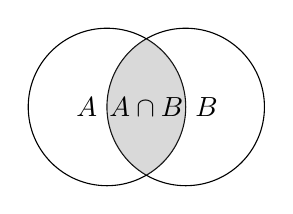
\begin{tikzpicture}
                \draw (0,0) circle[radius=1cm];
                \draw (1,0) circle[radius=1cm];
                \begin{scope}
                    \clip (1,0) circle [radius=1]; % B の形でクリッピングする
                    \fill[gray, opacity=0.3] (0,0) circle [radius=1]; % スコープの中で A を塗りつぶす
                \end{scope}
                \node at (0,0) [anchor=east] {$A$};
                \node at (1,0) [anchor=west] {$B$};
                \node at (0.5,0) [anchor=center] {$A\cap B$};
            \end{tikzpicture}
            \caption{共通部分$A\cap B$のVenn図}
        \end{figure}
    \clearpage
    \subsection{直積集合}
        QuuノートIにおいて, 実数$\mathbb{R}$は数直線ととらえることができると説明した. 同様にして, 二つの数直線を直交させてできる
        平面についても, この平面上の各点と二つの数直線の値とを対応付けることができるだろう. これは, 関数のグラフを書く時にすでに
        (直接言及されていないだけで)学んだことである. この平面の各点は, 二つの集合$\mathbb{R},\mathbb{R}$の各要素を対にしたもの
        全てを集めた集合といえよう.
        \begin{figure*}[h]
            \centering
            \begin{tikzpicture}
                \coordinate (P) at (1,2);
                \draw[->] (-1,0) -- (3,0);
                \draw[->] (0,-1) -- (0,3);
                \node at (P) [anchor = west] {$(1,2)$};
                \fill (P) circle[radius=0.1cm];
                \draw[dashed] (1,0) -- (P);
                \draw[dashed] (0,2) -- (P);
                \node at (1,0) [anchor=north] {$1$};
                \node at (0,2) [anchor=east] {$2$};
                \node at (3,0) [anchor=west] {$x$};
                \node at (0,3) [anchor=south] {$y$};
            \end{tikzpicture}
        \end{figure*}

        一般に, 二つの集合$A,B$に対して
        \begin{equation}
            A\times B =\{(a,b)\mid a\in A,b\in B\} \label{eq:集合論基礎:直積の定義}
        \end{equation}
        を$A$と$B$の\textbf{直積集合}\index{ちょくせきしゅうごう@直積集合}または単に\textbf{直積}\index{ちょくせき@直積}という. ここで, $(a,b)$は二つのもの$a,b$から作られる対となるもので, 
        これを\textbf{順序対}\index{じゅんじょつい@順序対}という. 順序対は集合と違って, $(a,b)\neq (b,a)$となる. つまり, 対の順序が違えばそれは違うものとみなす.
        二つの順序対$(a,b),(a',b')$が等しいのは$a=a',b=b'$となるときに限るとする. 

        直積を用いれば, 先ほど例で挙げた平面も$\mathbb{R}\times \mathbb{R}$と書けるとわかる. ただこの場合, 同一の集合の直積であるから
        簡単に$\mathbb{R}^2$と書くことにしよう. この記法は, 任意の集合$A$の直積$A\times A$についても用いられる. すなわち, $A\times A=A^2$である.

        直積の具体例を挙げよう. 例えば, $A=\{1,2,3\},B=\{2,3\}$とすると, $A\times B=\{(1,2),(1,3),(2,2),(2,3),(3,2),(3,3)\}$
        であり, $B\times A = \{(2,1),(2,2),(2,3),(3,1),(3,2),(3,3)\}$である. このように, 一般に直積では交換法則が成り立たない.

        直積$A\times B$において, $A,B$どちらか一方が空集合であれば順序対が存在しないので, この場合$A\times B$は空集合になる.\\

        今は二つの集合について, それぞれの要素から順序対を作っていた. これを$n$個の集合の場合に拡張しよう. $n$個の集合$A_1,A_2,\cdots,A_n$に対して, 
        それらの\textbf{直積集合}を
        \begin{equation}
            A_1\times A_2 \times \cdots \times A_n = \{(a_1,a_2,\cdots,a_n)\mid a_1\in A_1,a_2\in A_2,\cdots,a_n\in A_n\} \label{eq:集合論基礎:n個の直積の定義}
        \end{equation}
        によって定める. $(a_1,a_2,\cdots,a_n)$は順序対である. $n$個の場合でも二つの順序対が等しいのは, 並べられた各要素の値が等しい場合に限るとする.
        また, $A_1=A_2=\cdots=A_n=A$のとき, この直積集合を$A^n$とかく.\\

        直積は, もっと一般に集合系に対して定義される. しかし, 微分積分を学ぶ上では上記の定義で十分であるからここでは述べない.
        こちらも, 興味がある人は集合論の本を参考にしてほしい.
    \clearpage
    \subsection{写像}
        これまで扱ってきた関数は, 主に実数から実数に対応するものだった. 例えば, $f(x)=x^3$は, 全ての実数に対して定義され, 全ての実数に対応しているだろう.
        ここで議論したいのは, もっと一般に, 二つの集合間の対応である.
        
        二つの集合$X,Y$が与えられ, $X$の\underline{どの要素}に対しても, それぞれ$Y$の要素がただ一つ対応しているとき, この対応関係そのものを$X$から$Y$への\textbf{写像}\index{しゃぞう@写像}\footnote{対応関係自体を定義していないから, この定義は曖昧であるように感じる. この感覚は正常なものだ. 実際は, $X\times Y$の部分集合を対応関係と定義し, そのうち全ての$x\in X$に対して, $y\in Y$が一意的に存在するものを写像というのである.}と定義する.
        写像は, 関数や変換とも呼ばれたりするが, 全てまったくの同義語である. \footnote{関数は, 特に$X$が数の場合にいうようである.} $X$から$Y$の写像が$f$であることは, 次のように書かれる.
        \begin{equation}
            f:X\rightarrow Y \label{eq:集合論基礎:写像の書き方}
        \end{equation}
        このとき, $X$を$f$の\textbf{定義域}(始域)\index{しいき@始域}$Y$を\textbf{値域}(終域)\index{しゅういき@終域}という. また, 二つの写像$f:X\rightarrow Y, f':X'\rightarrow Y'$が\textbf{同じ写像である}\footnote{$A\subset X$に対して定義される$g:A\rightarrow Y$が任意の$x\in A$に対し, $f(x)=g(x)$であるとき, $g$を$f$の$A$の制限という. このとき$g=f\upharpoonright_A$とかく. また, $f$は$g$の拡張と呼ばれる.}とは, $X=X'\land Y=Y'$
        であって, $^\forall x\in X [f(x)=f'(x)]$であることをいう. このとき, $f=f'$とかく.

        $f:x\rightarrow y$によって, $x\in X$が$y\in Y$に対応することを$y=f(x)$とかく. このとき, $y$を$f$による$x$の\textbf{像}\index{ぞう@像}という. また, $x$を$f$による$y$の原像\index{げんぞう@原像}という.\\

        これまで扱ってきた関数の中には, $\sin(x^2)$のように, 関数の中に関数が入っているものがあった. これを合成関数といったわけだが, これを写像の場合にも考えてみる. すなわち, 集合$X,Y,Z$と, 
        二つの写像$f:X\rightarrow Y, g:Y\rightarrow Z$を考え, この合成写像なるものを考えてみよう. 写像$h:X\rightarrow Z$を, $h(x)=g(f(x))$として定める. この写像の各像は, $X$の要素を$Y$に飛ばし, 
        その像を$g$で$Z$の要素にとばしたものと一致する. これを\textbf{合成写像}\index{ごうせいしゃぞう@合成写像}といい, $g\circ f$とかく.
        
        合成写像に関しては, 交換法則は成り立たないが, 結合法則は成り立つ. すなわち
        \begin{equation}
            h\circ (g\circ f) = (h\circ g)\circ f \label{eq:集合論基礎:合成写像の結合法則}
        \end{equation}
        が成り立つ. ただし, $f,g,h$は, 集合$X,Y,Z,W$について, $f:X\rightarrow Y, g:Y\rightarrow Z, h:Z\rightarrow W$とする.
        \begin{proof}
            $x\in X$とする. このとき\[ [h\circ (g\circ f)](x)=h((g\circ f)(x))=h(g(f(x)))=(h\circ g)(f(x))=[(h\circ g)\circ f](x)\]
            が成り立つ. したがって等号が成り立つ.
        \end{proof}
        $f:X\rightarrow Y$を写像とする. $A\subset X$に対して, $\{f(a)\mid a\in A\}$を$f$による$A$の\textbf{像}\index{ぞう@像}といい, $f(A)$とかく. また, $B\subset Y$に対して, 
        $\{x\in X\mid f(x)\in B\}$を$f$による$B$の\textbf{逆像}\index{ぎゃくぞう@逆像}または\textbf{原像}\index{げんぞう@原像}といい, $f^{-1}(B)$と表す. 明らかに, $f(A)\subset Y,f^{-1}(B)\subset X$である.

        例えば, $f:\mathbb{R}\rightarrow \mathbb{R};x\mapsto x^2$\footnote{このように, 写像の像を具体的に$x\mapsto f(x)$と書くことがある.}として, $f([0,1])=[0,1]$である. 一方, $f^{-1}([0,1])=[-1,1]$である. 
        すなわち, この場合像と逆像は等しくない. 像も逆像も等しい例として, $f:\mathbb{R}\rightarrow \mathbb{R};x\mapsto x^3$がある. 先ほどと同じ部分集合の像を考えると$f([0,1])=[0,1]$であるし, $f^{-1}([0,1])=[0,1]$である
        から, この場合確かに等しい.
        \clearpage
        像と逆像に関しては以下の公式が成り立つ. ただし, $f:X\rightarrow Y$とし, $A_1,A_2\subset X,B_1,B_2\subset Y$とする.
        \begin{align}
            f(A_1 \cup A_2)&=f(A_1)\cup f(A_2) \label{eq:集合論基礎:像の和}\\
            f(A_1 \cap A_2)&\subset f(A_1)\cap f(A_2) \label{eq:集合論基礎:像の積}\\
            f^{-1}(B_1 \cup B_2)&=f^{-1}(B_1)\cup f^{-1}(B_2) \label{eq:集合論基礎:逆像の和}\\    
            f^{-1}(B_1 \cap B_2)&=f^{-1}(B_1)\cap f^{-1}(B_2) \label{eq:集合論基礎:逆像の積}\\    
            A_1 &\subset f^{-1}(f(A_1)) \label{eq:集合論基礎:像の逆像}\\
            f(f^{-1}(B_1)) &\subset B_1 \label{eq:集合論基礎:逆像の像}\\
            f(A_1)-f(A_2) &\subset f(A_1-A_2) \label{eq:集合論基礎:像の差}\\
            f^{-1}(B_1)-f^{-1}(B_2) &= f^{-1}(B_1-B_2) \label{eq:集合論基礎:逆像の差}
        \end{align}
        これも像と逆像の定義から導出できるから, 各自で証明してほしい. ここでは, \eqref{eq:集合論基礎:像の和}と\eqref{eq:集合論基礎:像の逆像}のみ証明しよう.
        \begin{proof}[\eqref{eq:集合論基礎:像の和}の証明.]
            \begin{equation*}
                f(A_1\cup A_2)=\{f(a)\mid a\in A_1\cup A_2\}=\{f(a)\mid a\in A_1\lor a\in A_2\}
            \end{equation*}
            であるから, $y\in f(A_1\cup A_2)$のとき, $y=f(a)$となる$a\in A_1$または$a\in A_2$が存在する. このときそれぞれ$y\in f(A_1),y\in f(A_2)$となるので
            $y\in f(A_1\cup A_2)\rightarrow y\in f(A_1)\cup f(A_2)$となる. 一方, $y\in f(A_1)\cup f(A_2)$のとき, $y\in f(A_1)$または$y\in f(A_2)$だから
            それぞれ$y=f(a)$となる$a\in A_1$もしくは$a\in A_2$が存在する. よって, $y\in f(A_1\cup A_2)$となるので, $y\in f(A_1)\cup f(A_2)\rightarrow y\in f(A_1\cup A_2)$である.
            従って, $f(A_1\cup A_2)=f(A_1)\cup f(A_2)$が示された.
        \end{proof}
        \begin{proof}[\eqref{eq:集合論基礎:像の逆像}の証明.]
            $a\in A_1$とする. このとき, 像の定義より$f(a)\in f(A_1)$が成り立つ. 一方逆像の定義から
            \begin{equation*}
                f^{-1}(f(A_1))=\{x\in X\mid f(x)\in f(A_1)\}
            \end{equation*}
            であるから, (集合の$\mid$より右の条件を満たすことより)$a\in f^{-1}(f(A_1))$である. よって, $A_1\subset f^{-1}(f(A_1))$
        \end{proof}
        \eqref{eq:集合論基礎:像の逆像}の証明において重要なのは, $a\in X$としたときに$f(a)\in f(A_1)$であっても, $a\in A_1$とは\underline{限らない}という点である. 例を挙げると, $f(x)=x^2$のとき
        $f([0,1])=[0,1]$であったが, $x=-1\in [-1,0]$であっても, $f(x)=(-1)^2=1\in [0,1]$が成り立っている. すなわち, $f(x)\in f([0,1])$となる$x$は$[-1,0]$内にも存在している.\\

        一般の写像に関する性質は以上でほとんどであるが, これだと\eqref{eq:集合論基礎:像の逆像}のような包含関係しか得られない. できる限り$=$であってほしいのが心情だろう.
        そこで, 写像の中でもとくに``都合の良い''ものを考えよう.

        写像$f:X\rightarrow Y$について, 次のように定める.
        \begin{enumerate}
            \item $f(X)=Y$であるとき, $f$は\textbf{全射}\index{ぜんしゃ@全射}または\textbf{上への写像}\index{うえへのしゃぞう@上への写像}であるという.
            \item $x_1,x_2\in X$について, $x_1\neq x_2$ならば$f(x_1)\neq f(x_2)$であるとき, $f$は\textbf{単射}\index{たんしゃ@単射}または\textbf{1対1写像}\index{1たい1しゃぞう@1対1写像}であるという.
            \item $f$が全射かつ単射であるとき, $f$は\textbf{全単射}\index{ぜんたんしゃ@全単射}であるという.
        \end{enumerate}
        写像$f$が全単射であれば, \eqref{eq:集合論基礎:像の和}から\eqref{eq:集合論基礎:逆像の差}のうち$\subset$であるものは等号が成り立つようになる. 
        全単射である写像の例として, 一次関数$f(x)=ax+b\quad (a\neq 0)$がある. これが全単射であることは容易に確かめられるから, これも各自で確かめてみるとよいだろう.
        \clearpage
        任意の集合$X_1\subset X_2$に対し, $X_1$の各要素$x$に対して, $i(x)=x$となる写像$i:X_1\rightarrow X_2$を\textbf{包含写像}\index{ほうがんしゃぞう@包含写像}という. 特に, $X_1=X_2=X$であるとき, 
        \textbf{恒等写像}\index{こうとうしゃぞう@恒等写像}という. 恒等写像はよく$\mathrm{id}_X$と書かれる. 恒等写像は全単射である. これも明らかである.\\

        写像$f:X\rightarrow Y$が全単射のとき, どの$y\in Y$に対しても$y=f(x)$となる$x\in X$が一意に定まるはずである. そこで, $y\in Y$に対して, $y=f(x)$を満たす$x\in X$
        を対応させることで, $Y$から$X$への写像が定まる. この写像を$f^{-1}:Y\rightarrow X$とかき, $f$の\textbf{逆写像}\index{ぎゃくしゃぞう@逆写像}という. 先ほど定義した逆像と言葉が似ているが, 異なる概念であるから気を付けてほしい.

        逆写像に関する基本的な定理には, 以下のものがある.
        \begin{screen}
            $f:X\rightarrow Y,\quad g:Y\rightarrow X$を写像とする. このとき$g\circ f = \mathrm{id}_X$であれば, $f$は単射で$g$は全射である.
            特に, $f\circ g = \mathrm{id}_Y$であれば, $f,g$はともに全単射で$g$は$f$の逆写像である.
        \end{screen}
        \begin{proof}
            $g\circ f=\mathrm{id}_X$であるとする. このとき, $x_1,x_2\in X$について$f(x_1)=f(x_2)$であるとする. このとき写像の定義から$g(f(x_1))=g(f(x_2))$である. 
            ところで, $g(f(x))=(g\circ f)(x)=\mathrm{id}_X(x)=x$であるから, $x_1=x_2$である. すなわち, $f(x_1)=f(x_2)\rightarrow x_1=x_2$だから, 対偶を取れば
            $x_1\neq x_2\rightarrow f(x_1)\neq f(x_2)$となって, $f$の単射性が示された. 次に, $g$が全射であることを示す. $x\in X$とする. このとき, $y=f(x)$と置くと, 
            $g(y)=g(f(x))=x$である. すなわち, $X$の任意の要素に対して, 対応元$y\in Y$が存在するから, $g$は全射である. まったく同様にして, $f\circ g= \mathrm{id}_Y$
            であれば, $f$は全射で$g$は単射である. 従って, $f,g$は全単射である. $g$が$f^{-1}$なのは逆写像の定義から明らかであろう.
        \end{proof}
        実は, 上の定理において$g\circ f$が単射であれば$f$は単射であり, $g\circ f$が全射であれば, $g$も全射である.\footnote{このとき, $f:X\rightarrow Y,g:Y\rightarrow Z$であっても成り立つ.} これは上の証明をすこし変えるだけだから, 読者への演習問題としよう.\\

        集合の列$A_1,A_2,\cdots,A_n$を考えよう. これらは, 各添え字$1,2,\cdots,n$に対して, 集合$A_1,A_2,\cdots,A_n$が対応している状態であるから, 添え字の集合$\{1,2,\cdots,n\}$からある集合族への一つの写像$A$が
        与えられていると考えられる. このように, ある空でない添え字の集合$\Lambda$からある集合族への写像$A$のことを, $\Lambda$上の\textbf{集合系}\index{しゅうごうけい@集合系}といい, 
        \begin{equation}
            (A_\lambda\mid\lambda \in \Lambda),\quad (A_\lambda)_{\lambda\in\Lambda} \label{eq:集合論基礎:集合系の定義1}
        \end{equation}
        とかく. 実用上は, 集合系も集合族も拘泥せず同じ集合の集合と考えてもよい. そのため, \eqref{eq:集合論基礎:集合系の定義1}は以下のようにも書かれる.
        \begin{equation}
            \{A_\lambda\mid \lambda\in\Lambda\} \label{eq:集合論基礎:集合系の定義2}
        \end{equation}
        集合系に対して, 和集合と共通部分を以下のように定める.
        \begin{align}
            \bigcup_{\lambda\in \Lambda} A_\lambda = \{x\mid {}^\exists \lambda \in \Lambda,x\in A_\lambda\} \label{eq:集合論基礎:集合系の和集合}\\
            \bigcap_{\lambda\in \Lambda} A_\lambda = \{x\mid {}^\forall \lambda \in \Lambda,x\in A_\lambda\} \label{eq:集合論基礎:集合系の共通部分}
        \end{align}
        \eqref{eq:集合論基礎:集合系の和集合}および\eqref{eq:集合論基礎:集合系の共通部分}はそれぞれ$\bigcup \{A_\lambda\mid\lambda\in\Lambda\},\bigcap \{A_\lambda\mid\lambda\in\Lambda\}$と書かれることもある. また, $\Lambda=\{1,2,\cdots,n\}$のときは, $\displaystyle\bigcup_{k=1}^{n},\bigcap_{k=1}^{n}$
        の記号を用いることもある. とくに, $\Lambda = \mathbb{N}$であれば, 
        \begin{equation*}
            \bigcup_{n=1}^{\infty}A_n,\quad \bigcap_{n=1}^{\infty}A_n
        \end{equation*}
        とかいてもよい. 

        集合系の各集合$A_\lambda$が集合$X$の部分集合であるとき, この集合系を$X$の\textbf{部分集合系}\index{ぶぶんしゅうごうけい@部分集合族}という. $\{A_\lambda\mid \lambda\in\Lambda\}$を$X$の部分集合系とする.
        このとき, 次の\textbf{de Morganの法則}\index{de Morganのほうそく@de Morganの法則}が成り立つ.
        \begin{align}
            \left(\bigcup_{\lambda\in\Lambda}A_\lambda\right)^c=\bigcap_{\lambda\in\Lambda}(A_\lambda)^c \label{eq:集合論基礎:一般のドモルガン1}\\
            \left(\bigcap_{\lambda\in\Lambda}A_\lambda\right)^c=\bigcup_{\lambda\in\Lambda}(A_\lambda)^c \label{eq:集合論基礎:一般のドモルガン2}
        \end{align}
        \eqref{eq:集合論基礎:一般のドモルガン2}は\eqref{eq:集合論基礎:一般のドモルガン1}からすぐでるから, \eqref{eq:集合論基礎:一般のドモルガン1}のみ示す.
        \begin{proof}
            \begin{equation*}
                x\in \left(\bigcup_{\lambda\in\Lambda}A_\lambda\right)^c \leftrightarrow \lnot [{}^\exists\lambda\in\Lambda,x\in A_\lambda]\leftrightarrow{}^\forall\lambda\in\Lambda,x\not\in A_\lambda\leftrightarrow{}^\forall\lambda\in\Lambda,x\in (A_\lambda)^c\leftrightarrow \bigcap_{\lambda\in\Lambda}(A_\lambda)^c
            \end{equation*}
            より等号が成り立つ.
        \end{proof}
        最後に, 集合系の極限にあたるものを定義しよう. $\mathbb{N}$を添え字の集合系とする集合系$\{A_n\mid n\in\mathbb{N}\}$に対して, 
        \begin{equation}
            \limsup_{n\to\infty}A_n=\bigcap_{k=1}^{\infty}\bigcup_{n=k}^\infty A_n \label{eq:集合論基礎:集合のlimsup}
        \end{equation}
        を\textbf{上極限集合}\index{うえきょくげんしゅうごう@上極限集合}という. 上極限集合は, 無限個の$A_n$に属す要素全てを集めた集合である. また, 
        \begin{equation}
            \liminf_{n\to\infty}A_n=\bigcup_{k=1}^{\infty}\bigcap_{n=k}^\infty A_n \label{eq:集合論基礎:集合のliminf}
        \end{equation}
        を\textbf{下極限集合}\index{したきょくげんしゅうごう@下極限集合}という. 下極限集合は, 有限個の$A_k$だけ除いて, それ以外を全て集めた集合である. 

        まず基本的なのは, 次の包含関係である.
        \begin{equation}
            \liminf_{n\to\infty}A_n\subset\limsup_{n\to\infty}A_n \label{eq:集合論基礎:limsupとliminfの包含関係}
        \end{equation}
        本によってはこの関係を明らかと書くようである. しかし, 私個人がこれを単に`明らか'とするのは納得がいかないから, 証明を与える.
        \begin{proof}
            すぐにわかることとして, $\displaystyle \bigcap_{n=k-1}^\infty A_n\subset\bigcap_{n=k}^\infty A_n$がある. したがって, 各$i\in\mathbb{N}$について, 
            \begin{equation*}
                \liminf_{n\to\infty} A_n=\bigcup_{k=1}^{\infty}\bigcap_{n=k}^\infty A_n=\bigcup_{k=i}^{\infty}\bigcap_{n=k}^\infty A_n
            \end{equation*}
            が成り立つ. 実際, $i$が大きくなることで生じる和集合の`漏れ'は, すべて$k\geq i$以降の$\bigcap_{k} A_n$に含まれている.
            また, $\displaystyle \bigcap_{n=k}^\infty A_n\subset A_k$であることもすぐわかる. したがって, 
            \begin{equation*}
                \bigcup_{k=i}^{\infty}\bigcap_{n=k}^\infty A_n\subset \bigcup_{k=i}^{\infty}A_k\Rightarrow \bigcap_{i=1}^\infty\bigcup_{k=i}^{\infty}\bigcap_{n=k}^\infty A_n\subset \bigcap_{i=1}^\infty\bigcup_{k=i}^{\infty}A_k=\limsup_{n\to\infty}A_n
            \end{equation*}
            であり, 左辺は$\displaystyle \bigcap_{i=1}^\infty\bigcup_{k=i}^{\infty}\bigcap_{n=k}^\infty A_n=\bigcup_{k=1}^{\infty}\bigcap_{n=k}^\infty A_n=\liminf_{n\to\infty}A_n$だから, $\displaystyle\liminf_{n\to\infty}A_n\subset\limsup_{n\to\infty}A_n$.
        \end{proof}
        \eqref{eq:集合論基礎:limsupとliminfの包含関係}において, 特に等式が成り立つ場合, これを\textbf{極限集合}\index{きょくげんしゅうごう@極限集合}といって, 
        \begin{equation}
            \lim_{n\to\infty}A_n=\limsup_{n\to\infty}A_n=\liminf_{n\to\infty}A_n \label{eq:集合論基礎:極限集合の定義}
        \end{equation}
        とかく. これらの概念はLebesgue積分論において重要である.
        \clearpage


    \clearpage
    \subsection{濃度}
            集合の個数と写像の関係について考えてみたい. 例えば, $\{1,2,3\}$と$\{p,i,e\}$という集合は, 個数が等しい. このとき, 二つの集合間に全単射が存在している. 例えば, $1\mapsto p,2\mapsto i,3\mapsto e$
            とすれば, これは明らかに全単射である. このように有限集合で個数が等しいときは全単射が存在している. 逆に, 二つの有限集合間に全単射が存在すれば, それらの要素数は等しいともいえるだろう.
            問題は無限集合である. 無限集合と有限集合の要素数が違うのはすぐわかるが, 無限集合同士ではどうだろうか. そもそも要素数が無限である場合, 要素数の比較などできるのだろうか.
            このような疑問を解消するために, 集合の濃度というものを考えてみよう. 二つの集合$A,B$の\textbf{濃度が等しい}\index{のうどがひとしい@濃度が等しい}とは, $A$から$B$への
            全単射が存在することである. このとき, $A\sim B$とかく. これは有限集合で考えていた集合の要素数の比較を拡張したものと考えてもよいだろう. 実際先ほどみたように, 有限集合で
            要素数が等しいときは, 全単射が存在するから, 濃度も等しいし, その逆も成り立っている. この濃度を用いて, 自然数の集合$\mathbb{N}$と偶数全体の集合$E$を比較してみよう.
            これは簡単で, 写像$f:\mathbb{N}\rightarrow E,n\mapsto 2n$を考えると, この写像は全単射であるから, $\mathbb{N}\sim E$が成り立つ. しかし, この結果は直感に反しているように感じているだろう.
            厳密性を欠いた表現をすれば, この結果は「自然数と偶数の`個数'が等しい」ということを意味しているのだから. 面白い例はほかにもある. 例えば, $\mathbb{N}\sim\mathbb{Z}$が成立する.
            これも直感に反しているようだが, 全単射は構成できてしまう. この全単射については, 演習問題で考えてもらうことにしよう.

            集合$A,B,C$について, 以下が成り立つ.
            \begin{enumerate}\renewcommand{\labelenumi}{(\arabic{enumi})}
                \item $A\sim A$
                \item $A\sim B$ならば$B\sim A$
                \item $A\sim B$かつ$B\sim C$ならば$A\sim C$
            \end{enumerate}
            \begin{proof}以下それぞれ証明を述べる. どれも示すことは, 全単射の存在である.
                \begin{enumerate}\renewcommand{\labelenumi}{(\arabic{enumi})}
                    \item 恒等写像$\mathrm{id}_A$を考えればよい.
                    \item 仮定より$A\rightarrow B$の全単射が存在して, 全単射の逆写像を考えればこれは$B\rightarrow A$の全単射である.
                    \item $A\rightarrow B$の全単射と$B\rightarrow C$の全単射の合成写像を考えれば, これは全単射である.
                \end{enumerate}
            \end{proof}
            二つの全単射の合成写像が全単射であることは直感的に明らかであるが, 厳密に証明をしておこう. より強い主張である以下の補題を示そう.
            \begin{screen}
                写像$f:X\rightarrow Y,g:Y\rightarrow Z$について, 以下が成立する.
                \begin{enumerate}\renewcommand{\labelenumi}{(\roman{enumi})}
                    \item $f,g$ともに単射であれば$g\circ f$も単射.
                    \item $f,g$ともに全射であれば$g\circ f$も全射.
                \end{enumerate}
            \end{screen}
            \begin{proof}以下に証明を述べる.
                \begin{enumerate}\renewcommand{\labelenumi}{(\roman{enumi})}
                    \item $x_1,x_2\in X,x_1\neq x_2$とする. $y_1=f(x_1),y_2=f(x_2)$と置くと, $f$の単射性から$y_1\neq y_2$である. また, $g$の単射性から$g(y_1)\neq g(y_2)$である. 
                    従って, $(g\circ f)(x_1)=g(f(x_1))=g(y_1)\neq g(y_2)=g(f(x_2))=(g\circ f)(x_2)$だから, $g\circ f$は単射.
                    \item 示すことは, $(g\circ f)(X)=Z$である. $f,g$は全射であるから$f(X)=Y,g(Y)=Z$が成立する. すなわち, 任意の$z\in Z$に対し, $z=g(y)$となる$y\in Y$および$y=f(x)$となる$x\in X$が存在する.
                    よって, $z=g(y)=g(f(x))=(g\circ f)(x)\in (g\circ f)(X)$が成り立つ. これより$Z\subset (g\circ f)(X)$であり, 写像の定義より$Z\supset (g\circ f)(X)$だから$Z=(g\circ f)(X)$, よって$g\circ f$は全射.
                \end{enumerate}
            \end{proof}
            全射の証明は, 以前述べた全射を示す証明とすこしやり方が違うように見えるだろう. 実際にはどちらのスタイルで証明してもらっても構わない. 個人的には, 今回の証明のほうがわかりやすい気がする.
            なおこの補題より, 全単射同士の合成写像が全単射であることは明らかであろう.\\

            全ての集合の濃度は互いに等しいとは限らない. この事実は重要である. 例えば以下が成り立つ.
            \begin{screen}
                \[\mathbb{N}\nsim \mathbb{R}\]
            \end{screen}
            これはCantorによって示された. 彼の有名な\textbf{対角線論法}\index{たいかくせんろんぽう@対角線論法}と呼ばれるアイデアを見てみよう.
            \begin{proof}
                背理法\footnote{証明すべき命題を否定した命題をもとに論理を導き, 矛盾を見つけることで元の命題を示す方法.}で示す. $\mathbb{N}\sim\mathbb{R}$であれば, 全単射$f:\mathbb{N}\rightarrow \mathbb{R}$が存在する.
                このとき(すべての)実数$f(n)$について, 10進法による無限小数展開を行うと, $f(n)=a_{n0}.a_{n1}a_{n2}\cdots a_{nn}\cdots$となる. ただし, 各$a_{nm}\quad(m=1,2,...)$が0から9までの整数,$a_{0n}\in \mathbb{Z}$で, 整数や有限小数は小数部分に0を続けるとする.
                例を挙げる. 例えば,$3.1415...$なら$a_{n0}=3,a_{n1}=1,a_{n2}=4,...$となる. $2.4$なら$a_{n0}=2,a_{n1}=4,a_{n2}=a_{n3}=\cdots=0$である. $n=1$から書き並べると以下のようになる.
                \begin{align*}
                    f(1)&=a_{10}.\bm{a_{11}}a_{12}a_{13}\cdots\\
                    f(2)&=a_{20}.a_{21}\bm{a_{22}}a_{23}\cdots\\
                    f(3)&=a_{30}.a_{31}a_{32}\bm{a_{33}}\cdots\\
                    \vdots
                \end{align*}
                小数部分の太字を見てほしい. この対角の数字を用いて, 新たな無限小数を作る. 具体的には, 各$a_{nn}$について
                \begin{equation*}
                    b_n=\left\{\begin{array}{lc}
                        1 & (a_{nn}は偶数)\\
                        2 & (a_{nn}は奇数)
                    \end{array}\right.
                \end{equation*}
                である$b_n$を用いて, 無限小数$b=0.b_{11}b_{22}b_{33}\cdots$をつくる. 重要なのは, 必ず$b_{n}\neq a_{nn}$となることである. この$b$は明らかに$b\in{\mathbb{R}}$であるが, 
                すべての$n\in \mathbb{N}$に対して, $f(n)\neq b$である. なぜなら, どの$n$についても小数第$n$位の数字が$b$と異なるからである.
                これは, $f$が全単射(全射)であることに矛盾する.
            \end{proof}
            自然数全体の集合$\mathbb{N}$と濃度が等しい集合を\textbf{可算集合}\index{かさんしゅうごう@可算集合}という. また, 有限集合と可算集合を合わせて\textbf{高々可算集合}\index{たかだがかさんしゅうごう@高々可算集合}
            という.\\

            集合の濃度を表す記号等を導入しておこう. 集合$A$に対して, $A$の\textbf{濃度}\index{のうど@濃度}を$|A|$または$\mathrm{card}A$を書く.
            集合の濃度とは, 濃度が等しい集合を集めた組のことである. 要素数$n$の有限集合の濃度は$n$とかく. また, 可算集合の濃度は$\aleph_0$(アレフ・ゼロ)とかき,  
            $\mathbb{R}$の濃度は$2^{\aleph_0}$とかく. 例えば, $|\varnothing|=0,|\mathbb{Z}|=\aleph_0$である.
            \clearpage

            我々が次に望むのは, 濃度を大小で比較できるようになることだろう. 集合$A,B$について, $A$から$B$への単射が存在するが, $B$から$A$への
            単射が存在しないとき, $A$は$B$より\textbf{濃度が小さい}\index{のうどがちいさい@濃度が小さい}, または, $B$は$A$より\textbf{濃度が大きい}\index{のうどがおおきい@濃度が大きい}という.
            $B$から$A$への単射が存在したときは何も言えないのか, と疑問に思うかもしれない. 実は, \textbf{Bernsteinの定理}\index{Bernsteinのていり@Bernsteinの定理}によって, $A$から$B$への単射と$B$から$A$への単射が存在するとき, 濃度が等しいことが濃度が等しいことが保障される.
            証明はここでは述べないから, 興味がある人は調べてみるとよい.\\

            最も重要なのは, 有理数の集合$\mathbb{Q}$が可算集合であることである. そのためにはまず, 二つの補題を示さなければならない.
            \begin{screen}
                集合$A,B$が$A\subset B$であれば, $A$から$B$への単射が存在する.
            \end{screen}
            \begin{proof}
                包含写像$i:A\rightarrow B$を考えると, これは明らかに単射であるから, 示された.
            \end{proof}

            \begin{screen}
                $\mathbb{Z}^2$は可算集合である.
            \end{screen}
            \begin{proof}
                $\mathbb{Z}=\{(m,n)\mid m,n\in\mathbb{Z}\}$は, 平面$\mathbb{R}^2$上の格子点の集合であるから, 下図のように対応をつけることで, $\mathbb{Z}^2=\{a_1,a_2,\cdots,a_n\cdots\}$
                とできる. したがって, $\mathbb{Z}^2$は可算集合である.
                \begin{figure}[h]
                    \centering
                    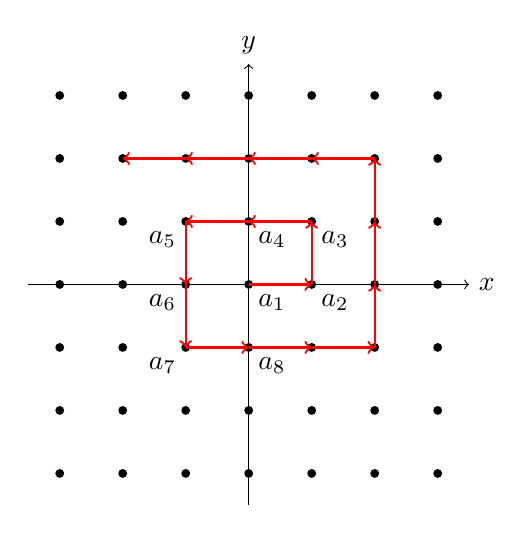
\begin{tikzpicture}[scale=0.8]
                        % 格子点を描画
                        \foreach \x in {-3,...,3} {
                            \foreach \y in {-3,...,3} {
                                \fill (\x,\y) circle (2pt);
                            }
                        }

                        % 軸を描画
                        \draw[->] (-3.5,0) -- (3.5,0) node[right] {$x$};
                        \draw[->] (0,-3.5) -- (0,3.5) node[above] {$y$};

                        % 編番号の経路を矢印で描画
                        \draw[thick,->,red] (0,0) -- (1,0);
                        \draw[thick,->,red] (1,0) -- (1,1);
                        \draw[thick,->,red] (1,1) -- (0,1);
                        \draw[thick,->,red] (0,1) -- (-1,1);
                        \draw[thick,->,red] (-1,1) -- (-1,0);
                        \draw[thick,->,red] (-1,0) -- (-1,-1);
                        \draw[thick,->,red] (-1,-1) -- (0,-1);
                        \draw[thick,->,red] (0,-1) -- (1,-1);
                        \draw[thick,->,red] (1,-1) -- (2,-1);
                        \draw[thick,->,red] (2,-1) -- (2,0);
                        \draw[thick,->,red] (2,0) -- (2,1);
                        \draw[thick,->,red] (2,1) -- (2,2);
                        \draw[thick,->,red] (2,2) -- (1,2);
                        \draw[thick,->,red] (1,2) -- (0,2);
                        \draw[thick,->,red] (0,2) -- (-1,2);
                        \draw[thick,->,red] (-1,2) -- (-2,2);

                        % 編番号を数列形式で表示
                        \node[below right] at (0,0) {$a_1$};
                        \node[below right] at (1,0) {$a_2$};
                        \node[below right] at (1,1) {$a_3$};
                        \node[below right] at (0,1) {$a_4$};
                        \node[below left] at (-1,1) {$a_5$};
                        \node[below left] at (-1,0) {$a_6$};
                        \node[below left] at (-1,-1) {$a_7$};
                        \node[below right] at (0,-1) {$a_8$};
                    \end{tikzpicture}
                    \caption{$a_1=(0,0)$として, 反時計回りに対応付けていく.}
                \end{figure}
            \end{proof}

            準備が整ったので, $\mathbb{Q}$が可算集合であることを示そう.
            \begin{proof}
                まず, $\mathbb{N}\subset \mathbb{Q}$より, $\mathbb{N}$から$\mathbb{Q}$への単射が存在する. 次に, $r\in \mathbb{Q}$は, 既約分数として$r=p/q\hspace{1mm}(p\in\mathbb{Z},b\in\mathbb{N})$
                の形にかける(整数$n$については, $q=1$として, $x=x/1$とかく). このとき, 
                \begin{equation*}
                    f:\mathbb{Q}\rightarrow\mathbb{Z}^2,\frac{p}{q}\mapsto (p,q)
                \end{equation*}
                は単射であるから, $\mathbb{Z}^2$が可算であるので$\mathbb{Z}^2$から$\mathbb{N}$への全単射が存在する. 以上より, $\mathbb{Q}$から$\mathbb{N}$への単射が存在するから, Bernsteinの定理より
                $\mathbb{Q}\sim \mathbb{N}$である.
            \end{proof}
            \clearpage
            最後に, 可算集合の部分集合は高々可算集合であることを示そう.
            \begin{proof}
                可算集合を$A$とする. $B\subset A$は有限集合か無限集合である. 有限集合であれば, それは高々可算集合であるから, $B$は無限集合であるとする.
                仮定より, 全単射$f:A\rightarrow \mathbb{N}$が存在する. よって, $f(B)=N\subset \mathbb{N}$と置くと, $B\sim N$である.
                $B$が無限集合であるから, $N$も無限集合である. したがって, 自然数の無限部分集合$N$が可算であることを示せばよい.
                写像$g:N\rightarrow\mathbb{N}$を考える. $g(n)$は集合$\{m\in N\mid m\leq n\}$の要素数とする. このとき, $g$は全単射である.
                \begin{enumerate}
                    \item 単射の証明.\\
                    $n_1,n_2\in N,n_1\neq n_2$とする. 対称性から$n_1<n_2$と仮定してもよい. このとき, $m\leq n_1$をみたす$m\in N$は$m\leq n_2$も満たし, 
                    後者の場合は$m=n_2$も条件を満たすから, $g(n_1)<g(n_2)$. したがって, $g(n_1)\neq g(n_2)$だから$g$は単射.
                    \item 全射の証明.\\
                    $n\in \mathbb{N}$とする. $N$は無限部分集合であるから, $n=g(k)$となる$k\in N$は存在する. ($N$の要素にはいくらでも大きい値がある.)
                    すなわち, $n\in g(N)$であるから, $\mathbb{N}\subset f(N)$. よって, $g$は全射.
                \end{enumerate}
                これより, $N$から$\mathbb{N}$への全単射が存在するから, $N\sim\mathbb{N}$. ゆえに, $B\sim \mathbb{N}$
            \end{proof}

    \clearpage
    \subsection{実数の連続性}
        ここでは, 実数の連続性について述べようと思う. 実数の性質を学ぶことは, 微分積分を行う上で大切だから, 少し難しいかもしれないが学んでいこう.\\

        \underline{全ての数}を$A,B$の二組に分けて, $A$に属する各数を$B$に属する各数よりも小さくできたとしよう. ただしこのとき$A,B$は空集合ではないとする. このような組み分け$(A,B)$
        をDedekindの\textbf{切断}(Dedekind cut)\index{せつだん@切断}といい, $A$を下組, $B$を上組という.

        ある数$s$について, $s$より小さい数全てを$A$, $s$よりも大きい数全てを$B$に入れるとする. $(A,B)$が切断であるためには, $s$も$A$または$B$に入っていなければならない.
        $s$が$A$に含まれるとき, $A$に最大値が存在し, $B$に最小値は存在しない.\footnote{例えば, $s=1$と考えると, $b\in B$は$b>1$である. 最小値が存在すると仮定し, それを$b$と置くと, 
        $b'=(b+1)/2$は, $b>b'>1$であり$b\in B$となる. これは$b$が$B$の最小値であることに矛盾する.} 逆に, $s$を$B$に入れれば, $A$に最大値は存在せず, $B$の最小値は存在する.
        このように, 任意の$s$について, それを境界とする切断を作ることができるが, この逆, すなわち次の定理が成り立つ.
        \begin{itembox}{Dedekindの定理\index{Dedekindのていり@Dedekindの定理}}
            実数の切断は, 下組と上組との境界として, 一つの数を確定する.
        \end{itembox}
        これが\textbf{実数の連続性}\index{じっすうのれんぞくせい@実数の連続性}である. 今後の論理の展開は, この定理が成り立つものとして, すなわち公理として認めて行う.

        大小の順序があるところ\footnote{この集合を順序集合という. もちろん実数も順序集合である.}には切断ができるが, この切断は次の三つの種類がある.

        \begin{enumerate}
            \item 下組に最大値が存在し, 上組に最小値が存在する. (leap)
            \item 下組に最大値が存在せず, 上組にも最小値が存在しない. (gap)
            \item 下組もしくは上組どちらかに端(最大値または最小値)が存在し, もう一方には端が存在しない. (連続)
        \end{enumerate}
        Dedekindの定理の主張とは, 実数の切断が3の切断に限られるということである.

        例えば, 自然数の切断を考えてみよう. このとき, 切断の下組と上組には必ず最大値および最小値が含まれている. すなわち, 自然数の切断は1のみである.
        逆に, 有理数の切断は1のようにできない. しかし, 2のようにはできる. 例えば, $s=\sqrt{2}$と取れば, $s\not\in \mathbb{Q}$であるから$s$は下組にも上組にも含まれないからである.
        もちろん, 3の切断もできる. これには有理数を$s$と取ればよい.\\

        次に, 最大値および最小値についてもう少し深掘りしよう. QuuノートIでは, 数列の有界について述べていた. 有界は一般の実数の部分集合についても定義できる.
        集合$A$に属する任意の数$a$に対して, $a\leq M$とできる実数$M$が存在するとき, $A$は\textbf{上に有界}\index{うえにゆうかい@上に有界}であるといい, この時の$M$を\textbf{上界}\index{じょうかい@上界}という.
        同様に, $a\geq m$とできる実数$m$が存在するとき, $A$は\textbf{下に有界}\index{したにゆうかい@下に有界}であるといい, この時の$m$を\textbf{下界}\index{げかい@下界}という.
        上にも下にも有界であるとき, $A$は\textbf{有界}\index{ゆうかい@有界}という.

        上界および下界は一つに定まらない. なぜなら, 上界が一つ存在すれば, それよりも大きい数も当然上界であるからである. 下界についても同様である.
        そこで, 上界のうち最小値と下界のうち最大値について考えてみる. 実は, $A$に最小値または最大値が存在しなくても, 上界の最小値または下界の最大値は存在する.
        この, 上界のうち最小である数を, $A$の\textbf{上限}\index{じょうげん@上限}といい, $\sup A$とかく. また, 下界のうち最大である数を, $A$の\textbf{下限}\index{かげん@下限}といい, $\inf A$とかく.

        $a=\sup A$であることと次の二つが同時に成り立つことは同値である.
        \begin{enumerate}
            \item $^\forall x\in A \left[x\leq a\right]$
            \item $^\forall r<a,{}^\exists x> r\left[x\in A\right]$
        \end{enumerate}
        1は$a$が$A$の上界であることを意味しており, 2で$a$より小さいどの数も上界になりえないこと\footnote{$r$は$a$より小さいが, そのとき$r$よりも大きい$x$が存在してその$x$が$A$に含まれていれば, $r$は上界でないのである.}を意味しているから, これは納得であろう.
        同様に, $a=\inf A$であることと次の二つが成り立つことも同値である.
        \begin{enumerate}
            \item $^\forall x\in A \left[x\geq a\right]$
            \item $^\forall r>a,{}^\exists x< r\left[x\in A\right]$
        \end{enumerate}

        例を挙げてみよう. 例えば, $[-1,1]$は最大値$1$, 最小値$-1$である. 一方$(-1,1]$は最大値$1$だが, 最小値は存在しない.
        しかし, 下限は存在して, それは$-1$である. $-1$は$(-1,1]$の下界であり, どの$r>-1$についても$r>x>-1$となる数が存在して, $x\in (-1,1]$
        であるから, 確かに存在している.

        なお, 上記の条件式は, 次のように書き換えることもできる. まず$a=\sup A$については
        \begin{enumerate}
            \item $^\forall x\in A \left[x\leq a\right]$
            \item $^\forall \varepsilon>0,{}^\exists x\in A \left[a-\varepsilon < x\right]$
        \end{enumerate}
        であり, $a=\inf A$については
        \begin{enumerate}
            \item $^\forall x\in A \left[x\geq a\right]$
            \item $^\forall \varepsilon>0,{}^\exists x\in A \left[x < a+\varepsilon\right]$
        \end{enumerate}
        となる.\footnote{それぞれ$r=a-\varepsilon,r=a+\varepsilon$と置けばよい.}

        \begin{figure}[h]
            \centering
            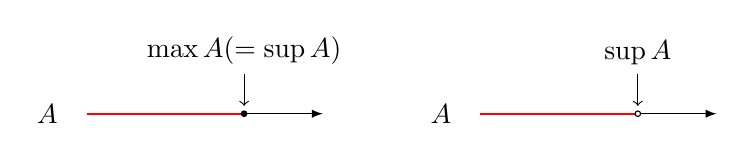
\begin{tikzpicture}
                \draw[-latex] (0,0) -- (3,0);
                \node at (-0.5,0) {$A$};
                \draw[red,thick] (0,0) -- (2,0);
                \draw[fill=black] (2,0) circle [radius=1pt]; 
                \draw[->] (2,0.5) -- (2,0.1);
                \node[above] at(2,0.5) {$\max A(=\sup A)$};

                \draw[-latex] (5,0) -- (8,0);
                \node at (4.5,0) {$A$};
                \draw[red,thick] (5,0) -- (7,0);
                \draw[fill=white] (7,0) circle [radius=1pt];
                \draw[->] (7,0.5) -- (7,0.1);
                \node[above] at(7,0.5) {$\sup A$};
            \end{tikzpicture}
            \caption{最大と上限の違い\\{\scriptsize 左の例では, 最大が存在しており, それは上限でもある. 一方右では最大は存在しない. しかし, 上限は存在する.}}
        \end{figure}
        \clearpage
        上限と下限で重要なのは, 次の定理である. 
        \begin{itembox}{Weierstrassの定理\index{Weierstrassのていり@Weierstrassの定理}}
            実数の部分集合$A$が上方(または下方に)有界ならば$A$の上限(または下限)が存在する.
        \end{itembox}
        これが先ほどのべた「上界の最小値...は存在する」の根拠, むしろそのものである. 
        \begin{proof}
            ここでは上限の存在のみ証明する.\footnote{下限の存在の証明は, 例えば解析概論 p.5を参照してほしい. ただ, その証明自体は上限の場合とほとんど同じである.}
            $A$が上に有界であるとき, その上界全てを$Y$, それ以外を$X$とすると, 切断$(X,Y)$を作ることができる.
            なぜなら, $X$に属する数はそのどの数も$A$の上界になりえない数であり, 必ず上界より小さいからである. Dedekindの定理によれば, この切断$(X,Y)$
            によって一つの実数$s$が確定する. $s$は$X$または$Y$のどちらかに必ず属している. ここで$s\in X$であるとしよう. このとき, $s$は
            $A$の上界になりえないから, $y>s$となる$y\in A$が存在するはずである. このとき, $y>t>s$となる$t$を考えると, $s$が$X$
            の最大値であることから, $t\in Y$である. しかし, $y>t$であるから, $t$は$A$の上界になりえず矛盾が生じる.
            したがって, $s\in Y$であり, このとき$s$は$Y$の最小値であるから, $A$の上限は存在し, それは$s$である.
        \end{proof}

        なお, 一般の順序集合にも上限および下限が定義できるが, そのとき必ずそれらが存在するとは限らないことも付記しておく.\\

        Weierstrassの定理を用いれば, QuuノートIで述べた単調で有界な数列が必ず収束する\footnote{以後, この定理を用いる際に限り, 単に上に(下に)有界であり単調増加(単調減少)な数列であっても``単調で有界な数列''ということがあるから注意してほしい.}
        ことに, 厳密な証明を与えることができる. 
        \begin{screen}
            (広義の)単調で有界な数列は必ず収束する.
        \end{screen}
        \begin{proof}
            数列$\{a_n\}$が単調増加で, 上に有界であるとする. このとき, 任意の$n$について$a_n<M$となる$M$が存在する.
            このとき集合$\{a_1,a_2,\cdots,a_n\cdots\}$は上に有界であるから, Weierstrassの定理よりこの上限は存在する.
            この上限を$\alpha$と置くと, 任意の$\varepsilon>0$に対して, ある$a_{N}$が存在して, $\alpha - \varepsilon < a_{N}$である.
            式を変形すると, $\alpha -a_{N}< \varepsilon$となる. ここで, $n>N$となる$n$について, $a_n>a_N$であるから, 
            $\alpha - a_{N} < \alpha - a_{n}$である. 以上より, 任意の$\varepsilon>0$に対して, ある$N>0$が存在して, $\alpha-a_{n}=|\alpha - a_{n}|<\varepsilon$
            となるから, この数列は収束して, その極限値は上限$\alpha$である. 数列が広義単調増加であっても, 全て等号が成り立つ場合を除けば同様に証明できる. 
            すべて等号が成り立つ場合は, その値を$\alpha$とすれば, 極限の定義よりそれは極限値である. 
            よって結局, 広義の単調増加で有界な数列は収束する. 単調減少についてもまったく同様に示せる.
        \end{proof}

        この定理を用いることで, 様々な命題を示すことができる. 
        
        \begin{itembox}{Archimedesの公理\index{Archimedesのこうり@Archimedesの公理}}
            任意の$x\in\mathbb{R}$に対して, $x<n$を満たす$n\in \mathbb{N}$が存在する.
        \end{itembox}
        \begin{proof}
            背理法で示そう. 仮にある$x\in\mathbb{R}$について, $x<n$となる自然数$n$が存在しないとしよう. 自然数$\mathbb{N}$を
            数列$\{n\}$と考えれば, これは単調増加な数列である. また, 背理法の仮定より, $x\geq n$である. したがってこの数列は
            単調で有界な数列であるから, 収束して, その値は上限$x$である. よって, $x-n<\varepsilon$が任意の$\varepsilon>0$で
            成立する. ここで$\varepsilon=1$とすると, $x<n+1$となるが, $n+1\in\mathbb{N}$であるから, 始めの仮定に矛盾する.
        \end{proof}

        Archimedesの公理から我々がよく知る, $1/n\rightarrow 0\quad (n\rightarrow\infty)$が導かれる. 普段我々はなんの断りもなしに
        この命題を認めていたのだった.

        \begin{screen}
            任意の$x\in\mathbb{R}$に対して, $m-1\leq x<m$を満たす$m\in\mathbb{Z}$が唯一存在する.
        \end{screen}
        \begin{proof}
            まず$x\geq 0$の場合を示す. Archimedesの公理より$x<n$を満たす$n\in\mathbb{N}$が存在する. このとき集合$M$を次のようにおく.
            \begin{equation*}
                M=\{l\in\mathbb{N}\mid x<l\leq m\}
            \end{equation*}
            $m\in M$であるから, $M$は空でない. また, $M$は無限集合ではない. よって, $M$の最小要素$m$をとれば, $m-1\leq x<m$とできる.
            $x<0$のときは, $-x>0$だから, $m-1\leq-x<m$となる$m$が存在する. よって, $-m+1\geq x>-m$であるから, 等号が成り立たない場合は
            $m\rightarrow -m+1$, 等号が成り立つ場合は$-m\rightarrow -m+1$を命題の表式に代入すれば成り立つことがわかる. 

            なお, これが唯一であることは$m_1<m<m_2$であるような整数$m_1,m_2$については成り立たないことを示せばよい. 
            $m_1\leq m-1\leq x<m\leq m_2+1$であるから, どちらも元の命題の式を満たさない.
        \end{proof}
        この命題の式を変形すれば, $m\leq x<m+1$が成り立つことがわかる. このときの$m$は$m=[x]$と書かれる. この記号$[\hspace{1mm}]$をガウス記号という. 

        Archimedesの公理と上の定理より, 次の非常に重要な命題が導かれる.
        \begin{itembox}{有理数の稠密性\index{ゆうりすうのちゅうみつせい@有理数の稠密性}}
            任意の$x,y\in\mathbb{R}\hspace{1mm}(x<y)$に対して, $x<r<y$を満たす有理数$r$が存在する.
        \end{itembox}
        \begin{proof}
            $y-x>0$であるから, Archimedesの公理より, $\frac{1}{y-x}<n$を満たす自然数$n$が存在する. よって$y-x>1/n$である. 
            また, 上記定理より, $m-1\leq nx < m$を満たす$m\in\mathbb{Z}$も存在する. したがって
            \begin{equation*}
                x<\frac{m}{n}=\frac{m-1}{n}+\frac{1}{n}<x+(y-x)=y
            \end{equation*}
            ところで, $m/n\in\mathbb{Q}$であるから, $r=m/n$が求める有理数である.
        \end{proof}
        有理数の稠密性
        \footnote{ちゅうみつと読む. 稠密とは簡単に言えば, 実数$x,y$の間にいくらでもその数が存在することをいう. 一般の稠密は, 次のように定義される(位相空間に関する多少の知識が必要). 
        $(X,\mathcal{O})$を位相空間とし, $A\subset X$とするとき, $A$が$X$で稠密であるとは, $A$の閉包$A^a$が$A^a=X$を満たすことをいう. 
        つまり, 有理数$\mathbb{Q}$の閉包は実数$\mathbb{R}$を包むのである.}
        を用いれば, 無理数の稠密性もすぐに示すことができる. これは簡単であるから演習問題に回すことにする.
        \clearpage
        
        今度は, 単調で有界な数列が収束することから, 切断とは別に実数を確定させる方法を考える.
        \begin{itembox}{区間縮小法\index{くかんしゅくしょうほう@区間縮小法}}
            閉区間$I_n=[a_n,b_n]\hspace{1mm}(n=1,2,\cdots)$において
            \begin{enumerate}
                \item 各区間$I_n$がその前の区間$I_{n-1}$に含まれる.
                \item $n$を十分大きくすれば, 各区間の幅$b_n-a_n$は十分小さくできる.
            \end{enumerate}
            とすれば, これら各区間に共通なただ一つの点が存在し, それは$\lim a_n=\lim b_n$である.
        \end{itembox}
        \begin{proof}
            始めの仮定1は, $a_n$が広義単調増加であり, $b_n$が広義単調減少な数列であることを意味する. さらに, $a_n\leq b_n$ということでもある.
            したがって, $a_n\leq b_1,a_1\leq b_n$であるから, $\{a_n\},\{b_n\}$は単調で有界な数列である. よって, 極限$\lim a_n =\alpha , \lim b_n=\beta$は
            存在する. したがって, $\alpha\leq \beta$が成り立つ. なぜなら, $\alpha>\beta$であるとすれば$\alpha -a_n<\varepsilon/2,b_n-\beta<\varepsilon/2$とできるから, 
            $0<\alpha-\beta<a_n-b_n+\varepsilon$となる. $\varepsilon=\alpha-\beta$と置けば,$0<a_n-b_n$すなわち$a_n>b_n$となり矛盾する.
            
            さて, 仮定2から, 任意の$\varepsilon>0$に対して, $b_n-a_n<\varepsilon$とできるような$n$が存在する. 
            \begin{equation*}
                a_n\leq \alpha\leq \beta\leq b_n
            \end{equation*}
            だから, $\varepsilon>b_n-a_n\geq b_n-\alpha\geq \beta - \alpha\geq0$となる. $\varepsilon$は任意であるから, $\beta=\alpha$である.
            任意の$n$について, $a_n\leq \alpha \leq b_n$であるから, $\alpha$は各$I_n$に含まれる. 
            
            仮に, $\alpha\neq \alpha'$である$\alpha'$が各区間で共通であるとしよう. このとき, $a_n\leq \alpha'\leq b_n$が任意の$n$に成り立つ.
            したがって, $0\leq \alpha'-a_n \leq b_n - a_n$であるから, $0\leq \alpha'-a_n<\varepsilon$である. これは$\lim a_n=\alpha'$を意味するが, 
            仮定$\alpha\neq\alpha'$に矛盾する. したがって, 各区間に共通する点は唯一で, それは$\alpha$である.
        \end{proof}

        最後に, 区間縮小法のみを仮定してDedekindの定理を導いてみよう.
        \begin{proof}
            切断$(A,B)$を考える. $A$に属する数$a$と$B$に属する数$b$を考える. このとき, 区間$I_0=[a,b]$の中間$\frac{a+b}{2}$は$A$か$B$のどちらかに属する.
            仮に, $A$に属するならば, $a_1=\frac{a+b}{2},b_1=b$と置き, $B$に属するなら$a_1=a,b_1=\frac{a+b}{2}$と置く. こうして新たな区間$I_1=[a_1,b_1]$ができる.
            $I_1$は$I$の右半分か左半分であり, その幅は$\frac{b-a}{2}$である. 次に, $I_1$の中間$\frac{a_1+b_1}{2}$についても同様に考え, $\frac{a_1+b_1}{2}$が
            $A$に属するならば, $a_2=\frac{a_1+b_1}{2},b_2=b_1$と置き, $B$に属するなら$a_2=a_1,b_2=\frac{a_1+b_1}{2}$と置く. このようにしてできる区間$I_2=[a_2,b_2]$も, 
            $I_1$の右半分か左半分であり, 幅は$\frac{b-a}{4}$である. この操作を繰り返せば, 区間の列$I_n$ができ, 各区間はその前の区間に含まれ, 区間の幅$\frac{b-a}{2^n}$は
            $n$が十分大きいときに十分小さくできるから, これは区間縮小法の条件を満たしている. よって, これら区間に共通なただ一つの点が存在する. 
            
            共通な点を$s$と置くことにする. $s\in A$であれば, それは$A$の最大である. なぜなら, 最大でないとき$s'\in A$が存在して$s<s'$であり, $b_n\rightarrow s$であるから, $b_n<s+\varepsilon$で, $\varepsilon=s'-s$と取れば, 
            $s<b_n<s'$とできる. しかし, $b_n\in B$であるから, $s'\in B$でなければならず, 矛盾である. このとき, $B$には最小が存在しない.
            仮に最小値$m$が存在していれば, $s<m$であるが, 先ほどと同様$\varepsilon=m-s$と取れば, $s<b_n<m$とできてしまう. $b_n\in B$であるから, これは$m$が$B$の最小であることに矛盾する.
            以上より, $s$が$A$も属していれば, $A$には最大が存在し, $B$に最小は存在しない. まったく同様にして, $s$が$B$に属するときも, $A$には最大が存在せず, $B$に最小は存在することが示される.
            すなわち, 切断$(A,B)$が与えられれば, 一つの数$s$が確定できたことになり, Dedekindの定理が示された. 
        \end{proof}
        \clearpage
        以上の結果をまとめよう. 我々は, Dedekindの定理を公理として, 実数の連続性に関する基本的な定理を導出してきた. そして最後には, 逆に区間縮小法からDedekindの定理を導くことも行った.
        ここからわかるのは, 以上で述べた四つの定理は互いに同等であるということである. すなわち, これらの定理のうちどれか一つを公理として認めれば, それ以外の定理は導くことができる.

        \begin{figure}[h]
            \centering
            \begin{tikzpicture}
                \node at (0,0) {Dedekindの定理};
                \node at (3,1.5) {Weierstrassの定理};
                \node at (0,3) {有界な単調数列の収束};
                \node at (-3,1.5) {区間縮小法};
                \draw [->] (0.5,0.5) -- (2.5,1);
                \draw [->] (2.5,2) -- (0.5,2.5);
                \draw [->] (-0.5,2.5) -- (-2.5,2);
                \draw [->] (-2.5,1) -- (-0.5,0.5);
            \end{tikzpicture}
            \caption{基本的な定理の関係}
        \end{figure}

        本によっては, 有界な単調数列の収束を公理としているものや, Weierstrassの定理を公理としているものがある. この理由は公理として選ばれなかったものは, 公理として選んだものから導かれるからである.

        なお, 以上の実数の性質は, このノートを含め, 断りなく使われることがあることに注意しておこう.
\clearpage
    \basicquestion 以下の問いに答えよ。

        \subsubsection*{問1} 次にうち, 正しい主張には〇, 間違っているものには×をつけよ.
            \begin{enumerate}
                \item $A\in 2^A$が成り立つ.
                \item $\{\varnothing\}=\varnothing$である.
                \item 関数$f(x)=\sin x$は, $\mathbb{R}$の範囲で全単射である.
                \item 命題$^\forall x\in X,{}^\exists y\in Y\left[P(x,y)\right]$と命題$^\exists y\in Y,{}^\forall x\in X\left[P(x,y)\right]$は互いに同値である.
            \end{enumerate}

        \subsubsection*{問2} $p\leftrightarrow q$を$\rightarrow,\leftarrow,\land$を用いずに表せ.

        \subsubsection*{問3}要素数が$n$である有限集合$A$の巾集合の要素数を求めよ.
        
        \subsubsection*{問4}数列$\{a_n\}$が有界である, を論理記号を用いて表せ.

        \subsubsection*{問5}公式\eqref{eq:集合論基礎:像の積}と\eqref{eq:集合論基礎:逆像の差}を示せ.

        \subsubsection*{問6}$\mathbb{N}\sim\mathbb{Z}$を示せ.

        \subsubsection*{問7}Archimedesの公理は次のように書けることを証明せよ.
        \begin{center}
            二つの実数$a,b>0$に対して, $na<b$となる自然数$n$が存在する.
        \end{center}

        \subsubsection*{問8}無理数の稠密性, すなわち, どんな二つの実数の間にも無理数が存在することを示せ.

        \subsubsection*{問9} 数列の上極限, 下極限を次のように定義する.
            \begin{equation}
                \limsup_{n\to\infty} a_n = \lim_{n\to\infty}\left(\sup_{k\geq n}a_k\right) \quad \liminf_{n\to\infty} a_n=\lim_{n\to\infty}\left(\inf_{k\geq n}a_n\right) \label{eq:集合論基礎:数列のlimsup,liminf}
            \end{equation}
            このとき, $\displaystyle\limsup a_n = \inf_{k\in\mathbb{N}}\left(\sup_{n\geq k}a_n\right),\quad \liminf a_n = \sup_{k\in\mathbb{N}}\left(\inf_{n\geq k}a_n\right)$となることを示せ.\\
            ただし, $\displaystyle \sup_{P(n)} a_n,\inf_{P(n)} a_n$とは, それぞれ$\{a_n\mid P(n)\}$の上限, 下限を表す.

\clearpage
\section{行列と行列式}
    ベクトルのイメージとその和・差について. 内積についても述べる. 外積はベクトル解析のときに述べる. 続いて, 行列についてその定義を述べ, 和・差・積について述べる.
    転置行列と逆行列についても述べる. 行列式は, 一般の定義を述べ, その後$2\times 2$と$3\times 3$について計算方法を述べる. 余因子展開についてその計算方法を述べる.
    \subsection{ベクトル}
        まずは, ベクトルについて簡単な説明をしよう. 基本的に平面の場合のみ説明するが, 空間の場合でも本質的な部分は同じである.

        \textbf{ベクトル}\index{べくとる@ベクトル}とは, `向き'と`大きさ'を持った量である. その最も身近な例は, 力学における速度, 力などだろう.
        これらはこれまで扱ってきた単なる数値(\textbf{スカラー}\index{すからー@スカラー})とは違う量である. このベクトルを図に示すと, 以下のようになる.
        \begin{figure}[h]
            \centering
            \begin{tikzpicture}
                \draw[-latex] (0,0) -- (1,1);
                \node[left] at (0,0) {$A$};
                \node[above] at (1,1) {$B$};
            \end{tikzpicture}
            \caption{ベクトルのイメージ}
        \end{figure}

        このベクトルは$\overrightarrow{AB}$と書かれる. 始点$A$から終点$B$までを結ぶ矢印というわけである. 正確に言うと, これはベクトルではないのだが, ひとまずのイメージはこの程度でよい. 
        以後ベクトルは上記のような表記ではなく, 太字表記$\bm{a},\bm{b},\dots$を主に用いる.

        ベクトルのうち, 大きさが0のベクトルを特別に\textbf{零ベクトル}\index{ぜろべくとる@零ベクトル}と呼び, $\bm{0}$と表記する. このベクトルは向きを持たないがこれもベクトルとみなす.

        次に考えたいのは, ベクトルの演算であろう. 具体的には, 四則演算について考えてみたい. ただ残念なことに, ベクトル同士の和・差・積については定義されているが, 商については定義されていないので, 
        ここでは和・差・積のみ考える.

        ベクトル同士の和は, 恐らく中学の理科で習ったであろう平行四辺形の法則をそのまま使う. すなわち以下の図のようになる.
        \begin{figure}[h]
            \centering
            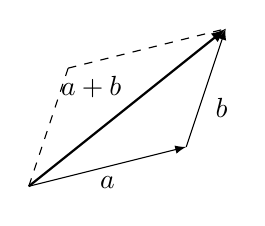
\begin{tikzpicture}
                \draw[-latex] (0,0) -- (2,0.5);
                \draw[-latex] (2,0.5) -- (2.5,2);
                \draw[-latex,thick] (0,0) -- (2.5,2);
                \node[below] at (1,0.25) {$\bm{a}$};
                \node[right] at (2.25,1) {$\bm{b}$};
                \node[above left] at (1.3,1) {$\bm{a}+\bm{b}$};
                \draw[dashed] (0,0) -- (0.5,1.5);
                \draw[dashed] (0.5,1.5) -- (2.5,2);
            \end{tikzpicture}
            \caption{ベクトルの和}
        \end{figure}
        このとき, 通常の数の演算のように交換法則と結合法則が成り立つ. これは図を描いてみればすぐわかるだろうから, ここでは詳しく述べない. また, 明らかに$\bm{a}+\bm{0}=\bm{a}$である.

        ベクトル$\bm{a}=\overrightarrow{AB}$に対し, その\textbf{逆ベクトル}\index{ぎゃくべくとる@逆ベクトル}を$-\bm{a}=\overrightarrow{BA}$と定義する. つまり, $\bm{a}$と向きが反対のベクトルが$-\bm{a}$である. 

        これより, ベクトルの差が定義できる. すなわち, $\bm{a}-\bm{b}$を$\bm{a}+(-\bm{b})$と定義することにする. $\bm{a}-\bm{a}=\bm{0}$であるので, $\bm{a}-\bm{b}$に$\bm{b}$を加えると$\bm{a}$となる.
        つまり, $\bm{a}-\bm{b}$は$\bm{b}$の終点を始点として, $\bm{a}$の終点を終点とするベクトルということになる.

        \begin{figure}[h]
            \centering
            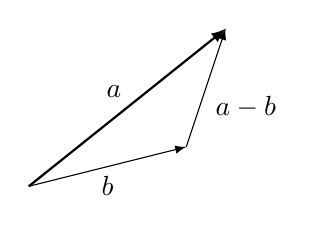
\begin{tikzpicture}
                \draw[-latex] (0,0) -- (2,0.5);
                \draw[-latex] (2,0.5) -- (2.5,2);
                \draw[-latex,thick] (0,0) -- (2.5,2);
                \node[below] at (1,0.25) {$\bm{b}$};
                \node[right] at (2.25,1) {$\bm{a-b}$};
                \node[above left] at (1.3,1) {$\bm{a}$};
            \end{tikzpicture}
            \caption{ベクトルの差}
        \end{figure}

        ベクトルの積については, 先にベクトルとスカラーの積について考えてみる. まず, $c>0$である実数$c$に対して, $c\bm{a}$を$\bm{a}$の大きさが$c$倍で, 向きが同じベクトルと定義する.
        $c<0$の場合は, 大きさは$c$倍であるが, 向きが$\bm{a}$と反対である. $c=0$の場合は$c\bm{a}=\bm{0}$である. また, $\bm{a}=\bm{0}$であれば, $c$の値にかかわらず$\bm{0}$となる.

        このとき, 次が成り立つ.
        \begin{align}
            &c(\bm{a}+\bm{b})=c\bm{a}+c\bm{b}\\
            &(c+d)\bm{a}=c\bm{a}+d\bm{a}\\
            &(cd)\bm{a}=c(d\bm{a})
        \end{align}
        単なる拡大または縮小であるから, 当然といえば当然である.

        ベクトル$\bm{a}$の大きさを$|\bm{a}|$と書くことにする. さて, ベクトル$\bm{a}$と$\bm{b}$の\textbf{内積}\index{ないせき@内積}(または\textbf{スカラー積}\index{すからーせき@スカラー積})は次のように定義される.
        \begin{equation}
            \bm{a}\cdot \bm{b}=|\bm{a}||\bm{b}|\cos\theta \label{eq:線形代数:内積の定義}
        \end{equation}
        $\theta$は二つのベクトルのなす角度である. これは, 二つのベクトルからスカラーを作る操作であり, ベクトルの積に相当する. ベクトルの積には内積とは別に外積というものもあるが, これはベクトル解析の部に任せることにして, ここでは内積の性質を見ていこう.

        まず, 次が成り立つ.
        \begin{align}
            &\bm{a}\cdot\bm{b}=\bm{b}\cdot\bm{a} \label{eq:線形代数:内積の交換法則}\\
            &\bm{a}\cdot(\bm{b}+\bm{c})=\bm{a}\cdot\bm{b}+\bm{a}\cdot\bm{c} \label{eq:線形代数:内積の分配法則}\\
            &\bm{a}\cdot\bm{a}=|\bm{a}|^2 \label{eq:線形代数:内積と大きさ}
        \end{align}
        このうち, \eqref{eq:線形代数:内積の交換法則}と\eqref{eq:線形代数:内積と大きさ}は定義からすぐわかる. 問題は\eqref{eq:線形代数:内積の分配法則}である. これを証明するには\textbf{ベクトルの成分表示}\index{べくとるのせいぶんひょうじ@ベクトルの成分表示}
        を使うのが簡単である.

        ベクトル$\bm{a}=\overrightarrow{AB}$をxy平面上で考える. このとき, $A(x_A,y_A),B(x_B,y_B)$と置くとき, $x_B-x_A,y_B-y_A$を$\bm{a}$の\textbf{成分}\index{せいぶん@成分}といい, 
        \begin{equation}
            \bm{a}=(x_B-x_A,y_B-y_A) \label{eq:線形代数:ベクトルの成分表示}
        \end{equation}
        とかく. また, この\eqref{eq:線形代数:ベクトルの成分表示}を\textbf{ベクトルの成分表示}\index{べくとるのせいぶんひょうじ@ベクトルの成分表示}という. これよりベクトルの大きさは$\sqrt{(x_B-x_A)^2+(y_B-y_A)^2}$とかける. これは三平方の定理からすぐわかる.
        また, ベクトルの和, 差はそれぞれ対応する成分同士で行い, スカラー倍は各成分をそれぞれスカラー倍すればよい.

        これを用いて, \eqref{eq:線形代数:内積の定義}をベクトルの各成分で表してみよう. $\bm{a}=(a_x,a_y),\bm{b}=(b_x,b_y)$とする.
        このとき$|\bm{a}|=\sqrt{a_x^2+a_y^2},\quad|\bm{b}|=\sqrt{b_x^2+b_y^2},\quad |\bm{a}-\bm{b}|=\sqrt{(a_x-b_x)^2+(a_y-b_y)^2}$である.
        \clearpage
        また, $\cos\theta$については, 下図\ref{fig:線形代数:内積の証明用}より余弦定理を用いて, 
        \begin{equation*}
            \cos\theta = \frac{|\bm{a}|^2+|\bm{b}|^2-|\bm{a}-\bm{b}|^2}{2|\bm{a}||\bm{b}|}
        \end{equation*}
        と書けるから, \eqref{eq:線形代数:内積の定義}は
        \begin{equation*}
            \bm{a}\cdot\bm{b}=\frac{1}{2}\left(|\bm{a}|^2+|\bm{b}|^2-|\bm{a}-\bm{b}|^2\right)=\frac{1}{2}\left\{a_x^2+a_y^2+b_x^2+b_y^2-(a_x-b_x)^2+(a_y-b_y)^2\right\}
        \end{equation*}
        となり, これを計算すると
        \begin{equation}
            \bm{a}\cdot\bm{b}=a_xb_x+a_yb_y \label{eq:線形代数:内積の成分表示}
        \end{equation}
        この表式は内積の計算をしばしば簡単にする. これを用いれば, \eqref{eq:線形代数:内積の分配法則}は, $\bm{c}=(c_x,c_y)$として, 
        \begin{equation*}
            (左辺)=\bm{a}\cdot (b_x+c_x,b_y+c_y)=a_x(b_x+c_x)+a_y(b_y+c_y)=(a_xb_x+a_yb_y)+(a_xc_x+a_xc_y)=(右辺)
        \end{equation*}
        と簡単に証明にできる.

        \begin{figure}[h]
            \centering
            \begin{tikzpicture}
                \draw[-latex] (0,0) -- (2,-0.5);
                \draw[-latex] (2,-0.5) -- (2.5,2);
                \draw[-latex] (0,0) -- (2.5,2);
                \node[below] at (1,-0.25) {$\bm{b}$};
                \node[right] at (2.25,0.75) {$\bm{a-b}$};
                \node[above left] at (1.3,1) {$\bm{a}$};

                \draw (0,0) coordinate (A) -- (2,-0.5) coordinate (B) -- (2.5,2) coordinate (C);
                \draw pic["$\theta$", draw, <->, font=\footnotesize, angle eccentricity=1.5, angle
                radius=0.5cm] {angle=B--A--C};
            \end{tikzpicture}
            \caption{ベクトルと三角形} \label{fig:線形代数:内積の証明用}
        \end{figure}

        先ほどのベクトルの成分表示からわかるように, ベクトル$\bm{a}=\overrightarrow{AB}$は, $A,B$の絶対位置にはよらず, 相対位置(二つの点の位置関係)にのみ依存している.
        また, 本来のベクトルの定義では, ベクトルは`向き'と`大きさ'を持つ量として定義されている. すなわち, 同じ向きと大きさを持つベクトルであれば, \underline{その二つのベクトルがどの位置にあろうとも
        同一視しなければならない.}

        一方, 特定の点に作用するベクトルを\textbf{束縛ベクトル}\index{そくばくべくとる@束縛ベクトル}\footnote{逆に, 今までの始点が固定されていないベクトルは\textbf{自由ベクトル}\index{じゆうべくとる@自由ベクトル}という.}という. 束縛ベクトルには, 例えばモーメントや, 次に説明する位置ベクトルなどがある.

        xy平面上の点$P(x,y)$について, $P$の\textbf{位置ベクトル}\index{いちべくとる@位置ベクトル}を$\bm{r}=(x,y)$と定義する. xy平面上の全ての点に対して, 対応する位置ベクトルは存在し, 逆に全てのベクトルは
        xy平面上のある点の位置ベクトルになっている. この位置ベクトルは, 力学でも用いるし, このあとのベクトル解析でもひんぱんに用いる.

        次は, ベクトルについて平行と垂直を考えてみよう. 二つのベクトルが\textbf{平行}\index{へいこう@平行}であるとは, それらのベクトルの向きが同じが反対であることをいう. すなわち,
        \begin{equation}
            \bm{a}/\!/\bm{b}\Leftrightarrow {}^\exists k\in\mathbb{R}\left[\bm{b}=k\bm{a}\right] \label{eq:線形代数:ベクトルの平行}
        \end{equation}
        である. また, 二つのベクトルが\textbf{垂直}\index{すいちょく@垂直}であるとは, 二つのベクトルのなす角度が$\frac{\pi}{2}$であることをいう. つまり, $\cos\theta=0$であるから, 
        \begin{equation}
            \bm{a}\perp\bm{b}\Leftrightarrow \bm{a}\cdot\bm{b}=0 \label{eq:線形代数:ベクトルの垂直}
        \end{equation}
        となる. つまり, 二つのベクトルが垂直であるかどうかを調べるためには, 内積が0であるかどうかをみればよいのである.
        \clearpage
        ベクトルで重要なのは次の二つの不等式である.
        \begin{align}
            &|\bm{a}\cdot\bm{b}|\leq |\bm{a}||\bm{b}| &\quad(\text{schwarzの不等式}) \label{eq:線形代数:シュワルツの不等式}\\
            &|\bm{a}+\bm{b}| \leq |\bm{a}|+|\bm{b}| &\quad(\text{三角不等式}) \label{eq:線形代数:三角不等式}
        \end{align}
        \eqref{eq:線形代数:シュワルツの不等式}は, $\cos\theta$の値域から明らかである. よって, \eqref{eq:線形代数:三角不等式}について示す.

        \begin{proof}
            左辺を二乗すると, \eqref{eq:線形代数:内積と大きさ}より
            \begin{equation*}
                |\bm{a}+\bm{b}|^2 = (\bm{a}+\bm{b})\cdot (\bm{a}+\bm{b})=\bm{a}\cdot\bm{a} + 2\bm{a}\cdot\bm{b}+\bm{b}\cdot\bm{b}\leq|\bm{a}|^2+|\bm{b}|^2+2|\bm{a}||\bm{b}|=(|\bm{a}|+|\bm{b}|)^2
            \end{equation*}
            となるから, 両辺$\sqrt{\hspace{1mm}}$を取ればよい.\footnote{両辺のルートの中身が正であるから, このようにしてもよい.} なお, 途中の不等式は, やはり$\cos\theta$の値域から変形した.
        \end{proof}

        最後に, 基本ベクトルについて述べよう. まず, 大きさが1であるベクトルのことを\textbf{単位ベクトル}\index{たんいべくとる@単位ベクトル}という. ベクトル$\bm{a}\neq\bm{0}$に対して, $\bm{e}=\bm{a}/|\bm{a}|$
        は単位ベクトルとなる. このように, ベクトルの大きさを1にすることを\textbf{正規化する}\index{せいきかする@正規化する}という. 単位ベクトルは, ベクトルの`向き'のみ抽出したものといえるだろう.
        
        単位ベクトルのうち, 次のベクトルを考える.
        \begin{equation}
            \bm{i}=(1,0),\quad \bm{j}=(0,1) \label{eq:線形代数:平面の基本ベクトル}
        \end{equation}
        このベクトルをそれぞれ, $x$方向, $y$方向の\textbf{基本ベクトル}\index{きほんべくとる@基本ベクトル}という. 基本ベクトルは明らかに単位ベクトルである.
        基本ベクトルを用いれば, 任意のベクトルはこれらの\textbf{線形結合}\index{せんけいけつごう@線形結合}で表せる. すなわち, 任意のベクトル$\bm{a}=(a_x,a_y)$は次のように書ける.
        \begin{equation}
            \bm{a}=a_x\bm{i}+a_y\bm{j} \label{eq:線形代数:基本ベクトルの線形結合}
        \end{equation}
        これは, 基本ベクトルが\textbf{線形独立}\index{せんけいどくりつ@線形独立}であることともかかわってくるのだが, ここでは述べない.\\

        以上が, 平面のベクトルに関する基本的な内容である. 通常の線形代数では, 直線の(ベクトル)方程式なども範囲に含まれるのだが, ここではあくまで微分積分がメインなので, あまり深く立ち入らないことにする. 
        なお, 以上の議論は空間ベクトルの場合もほとんどそのまま適用される. ただし, 成分表示などは2つから3つ増えることに注意. また, 基本ベクトルは$\bm{i}=(1,0,0),\bm{j}=(0,1,0),\bm{k}=(0,0,1)$の3つとなる.

        補足として, ここでは行ベクトル(横ベクトル)として扱ったが, 線形代数の教科書では基本的に列ベクトル(縦ベクトル)で書く場合が多いようである. これはおそらく次にやる行列の積が念頭にあるのだろう. 
        私はあまり線形代数に詳しくないので厳密なことはよくわからないが, とりあえず今は列ベクトルで書こうが行ベクトルで書こうが気にしなくてよいのではないだろうか.
    \clearpage
    \subsection{行列}
        ここでは行列について述べる. 行列は, 複数のベクトルを縦または横に並べて作ることができる, 複数の数の集まりである. ただ, ベクトルが物理量を表すのに対し, 行列は単なる数の集まりである. この違いを意識するには相対論の部を読んでみるとよいから, ここでは
        そこまで深く考えず行列の定義と演算法について扱う.

        
        まず, $mn$個の数$a_{ij}(i=1,2,\dots,m,j=1,2,\dots,n)$を次のように並べ, かっこで囲んだものを考える.
        \begin{equation}
            A=\begin{pmatrix}
                a_{11} & a_{12} & \cdots & a_{1n}\\
                a_{21} & a_{22} & \cdots & a_{2n}\\
                \hdotsfor{4}\\
                a_{m1} & a_{m2} & \cdots & a_{mn}
            \end{pmatrix} \label{eq:線形代数:行列の定義}
        \end{equation}
        これを, \textbf{$m$行$n$列の行列}\index{ぎょうれつ@行列}, または単に行列という. 行列の横の並びを行, 縦の並びを列という.
        また, 第$i$行と第$j$列が交わる要素$a_{ij}$を, この行列$A$の\textbf{$(i,j)$成分}\index{i,jせいぶん@$(i,j)$成分}という.

        特に, $1\times n$行列は, $n$次元行ベクトルであり, $m\times 1$行列は, $m$次元列ベクトルである. これまで扱ってきた平面のベクトルは$1\times 2$行列だったというわけである.

        行列は, 基本的に大文字で表される. ただし, やはりベクトルは特別に太字の記号のままとする. 全ての成分が0である行列は, \textbf{零行列}\index{ぜろぎょうれつ@零行列}といい, $O$とかく.

        二つの行列について, 行の数と列の数がともに等しいときは, それらは同じ型という. 二つの行列が同じ型であれば, それらが等しい行列であるかどうかを考えることができる. 二つの行列が等しいとは, それぞれの$(i,j)$成分
        がすべて等しいことをいう.

        行列の中で, $m=n$, つまり行の数と列数が一致しているものを$m$次の\textbf{正方行列}\index{せいほうぎょうれつ@正方行列}という. 正方行列$A=(a_{ij})$\footnote{\eqref{eq:線形代数:行列の定義}の書き方は場所を取るから, このように表記している.}
        について, $a_{kk}$の成分を\textbf{対角成分}\index{たいかくせいぶん@対角成分}という. 対角成分以外がすべて0である行列を\textbf{対角行列}\index{たいかくぎょうれつ@対角行列}という.
        特に, 対角行列の対角成分が全て1である行列を\textbf{単位行列}\index{たんいぎょうれつ@単位行列}といい, $E$と表す.\\

        ベクトルと同様, 行列にも和・差・積が定義できる. ただし和・差は同じ型の行列間においてのみ定義され, $(a_{ij})\pm(b_{ij})=(a_{ij}\pm b_{ij})$となる.
        つまり, 各成分同士を足す(引く)だけである. 当然このときも交換法則と結合法則が成り立つ.

        行列の差の特別な場合として, $O-A$を$-A$と書くことにする. この行列は, $A$の各成分が$-1$倍されたものである. ベクトルと同様に, スカラーと行列の積は$k(a_{ij})=(ka_{ij})$と定義される. 
        よって, $(-1)A=-A$ということになる. ベクトルと同じく, 次の関係が成り立つ.

        \begin{align}
            &c(A + B)=cA + cB\\
            &(c+d)A=cA + dA\\
            &(cd)A=c(dA) 
        \end{align}

        これも, 簡単な計算からすぐわかるだろうから証明は省略する.
        \clearpage
        行列の積を考える前に, ベクトルの内積を行列を用いて表すことを考えてみる. 簡単な場合として, 二次元の場合で考えよう.
        行ベクトル$\begin{pmatrix}
            a_1 & a_2 
        \end{pmatrix}$と, 列ベクトル$\begin{pmatrix}
            b_1\\b_2
        \end{pmatrix}$について, これらの積を次のように定める.
        \begin{equation*}
            \begin{pmatrix}
            a_1 & a_2 
        \end{pmatrix}\begin{pmatrix}
            b_1\\b_2
        \end{pmatrix}=a_1b_1+a_2b_2
        \end{equation*}
        これはまさに内積である. 以前, 行列は複数のベクトルを並べて作れると述べた. これに則って, $m\times l$の行列と$l\times n$の行列の積を次のように定める.
        \begin{equation}
            \begin{pmatrix}
                a_{11} & a_{12} & \cdots & a_{1l}\\
                a_{21} & a_{22} & \cdots & a_{2l}\\
                \hdotsfor{4}\\
                a_{m1} & a_{m2} & \cdots & a_{ml}
            \end{pmatrix}
            \begin{pmatrix}
                b_{11} & b_{12} & \cdots & b_{1n}\\
                b_{21} & b_{22} & \cdots & b_{2n}\\
                \hdotsfor{4}\\
                b_{l1} & b_{l2} & \cdots & b_{ln}
            \end{pmatrix}                    
            =\begin{pmatrix}
                \sum a_{1k}b_{k1} & \sum a_{1k}b_{k2} & \cdots & \sum a_{1k}b_{kn}\\
                \sum a_{2k}b_{k1} & \sum a_{2k}b_{k2} & \cdots & \sum a_{2k}b_{kn}\\
                \hdotsfor{4}\\
                \sum a_{mk}b_{k1} & \sum a_{mk}b_{k2} & \cdots & \sum a_{mk}b_{kn}
            \end{pmatrix} \label{eq:線形代数:行列の積}
        \end{equation}
        ただし, 和の記号$\sum$は$k=1$から$k=l$までの和を取ることを意味する.

        計算例をいくつか挙げよう.
        \begin{align*}
            &\begin{pmatrix}
                2  & 5 \\
                -3 & 1
            \end{pmatrix}
            \begin{pmatrix}
                0 &  3 \\
                1 & -1
            \end{pmatrix}=\begin{pmatrix}
                2\times 0 +5\times 1 & 2\times 3 + 5\times -1\\
                -3\times 0 + 1\times 1 & -3\times 3+1\times -1
            \end{pmatrix}
            =\begin{pmatrix}
                5 & 1\\
                1 & -10
            \end{pmatrix}\\
            &\begin{pmatrix}
                1 & 1 \\
                5 & 0 \\
                1 & 4
            \end{pmatrix}
            \begin{pmatrix}
                2 & 1 & 3 \\
                0 & 5 & 0
            \end{pmatrix}=\begin{pmatrix}
                1\times 2 +1\times 0 & 1\times 1 + 1\times 5 & 1\times 3 + 1\times 0\\
                5\times 2 + 0\times 0 & 5\times 1+0\times 5 & 5\times 3 + 0\times 0\\
                1\times 2 + 4\times 0 & 1\times 1+4\times 5 & 1\times 3 + 4\times 0
            \end{pmatrix}
            =\begin{pmatrix}
                2 & 6 & 3\\
                10 & 5 & 15\\
                2 & 21 & 3
            \end{pmatrix}\\
            &\begin{pmatrix}
                3 \\ -2 \\ 1
            \end{pmatrix}
            \begin{pmatrix}
                4 & 0 & 5
            \end{pmatrix}
            =\begin{pmatrix}
                3 \times 4 & 3\times 0 & 3\times 5\\
                -2\times 4 & -2 \times 0 & -2 \times 5\\
                1 \times 4 & 1 \times 0 & 1 \times 5
            \end{pmatrix}
            =\begin{pmatrix}
                12 & 0 & 15 \\
                -8 & 0 & -10\\
                4  & 0 & 5  \\ 
            \end{pmatrix}
        \end{align*}

        行列の積は, まず覚えずらい上に, 計算ミスが多発しやすい. 何回か練習することをお勧めする. また, 積の計算の際には, 次のように`補助線'を引くと計算しやすい.
        \begin{equation*}
            \left(
            \begin{array}{ccc} 
                2 & 1 & 3 \\ \hline
                0 & 5 & 0 
            \end{array} 
            \right)
            \left(
            \begin{array}{c|c} 
            1 & 1\\
            5 & 0\\
            1 & 4 
            \end{array} 
            \right)
            =\begin{pmatrix}
                10 & 14\\
                25 & 0
            \end{pmatrix}
        \end{equation*}

        上記の計算を見ればわかるように, 行列の積$AB$は, $A$の列の数と$B$の行の数が一致するときのみ定義される. また, 行列の積は可換ではない. 
        すなわち, 一般には$AB= BA$は成立しない. しかし, それでも分配法則と結合法則は成り立つ. ただし, どれも和と積が計算できる場合である.
        \begin{align}
            &(A+B)C = AC + BC \\
            &C(A+B) = CA + CB\\
            &(AB)C = A(BC)
        \end{align}
        最初の式だけ証明をしておこう. それ以外も同様にできる.
        \begin{proof}
            $A=(a_{ij}),B=(b_{ij}),C=(c_{ij})$と置く. このとき,
            \begin{equation*}
                (A+B)C=(a_{ij}+b_{ij})C = \left(\sum_{k=1}^{l} (a_{ik}+b_{ik})c_{kj}\right)=\left(\sum a_{ik}c_{kj}+\sum b_{ik}c_{kj}\right)=\left(\sum a_{ik}c_{kj}\right)+\left(\sum b_{ik}c_{kj}\right)=AB+BC
            \end{equation*}
            が成り立つ.
        \end{proof}
        \clearpage
        任意の行列について, 対応する単位行列との積は必ず元の行列となる.
        \begin{equation}
            AE = A,\quad EA = A
        \end{equation}
        ここでいう`対応する'とは, $A$と列の数もしくは行の数が等しいという意味である.

        \begin{proof}
            $A=(a_{ij})$と置く. ここで次の記号を導入する. 
            \begin{equation}
                \delta_{ij} = \left\{\begin{array}{cc}
                    1 & (i=j)\\ 0 & (i\neq j)
                \end{array}\right. \label{eq:線形代数:クロネッカーのデルタ}
            \end{equation}
            これを\textbf{Kroneckerのデルタ}\index{Kronockerのでるた@Krnoneckerのデルタ}という. これを用いれば, $E=(\delta_{ij})$と書ける. これより
            \begin{align*}
                &AE=\left(\sum_{k=1}^{l}a_{ik}\delta_{kj}\right)=(a_{ij}\delta_{jj})=(a_{ij})=A\\
                &EA=\left(\sum_{k=1}^{l}\delta_{ik}a_{kj}\right)=(\delta_{ii}a_{ij})=(a_{ij})=A
            \end{align*}
            となる.
        \end{proof}

        任意の行列に対し, $AO=O,OB=O$が成り立つ. これは明らかである. しかし, $A\neq O,B\neq O$であっても$AB=O$が成立することがある.
        例えば
        \begin{equation*}
            \begin{pmatrix}
                1 & 1 \\ 2 & 2
            \end{pmatrix}
            \begin{pmatrix}
                -3 & 3 \\ 3 & -3
            \end{pmatrix}
            =\begin{pmatrix}
                0 & 0 \\ 0 & 0
            \end{pmatrix}
        \end{equation*}
        である. このような$A,B$を\textbf{零因子}\index{ぜろいんし@零因子}という.\\

        行列の行と列を入れ替えることで, 新たな行列を作ることができる. この操作を\textbf{転置する}\index{てんちする@転置する}といい,
        $A$を転置した行列を$^t\!A$とかき, $A$の\textbf{転置行列}\index{てんちぎょうれつ@転置行列}という.

        例えば
        \begin{equation*}
            ^t\!\begin{pmatrix}
                1 & 2 & 3\\
                4 & 5 & 6
            \end{pmatrix}
            =\begin{pmatrix}
                1 & 4\\
                2 & 5\\
                3 & 6
            \end{pmatrix}
            ,\quad
            ^t\!\begin{pmatrix}
                5 & -3 & 8
            \end{pmatrix}
            =\begin{pmatrix}
                5 \\ -3 \\ 8
            \end{pmatrix}
            ,\quad
            ^t\!E = E
        \end{equation*}
        転置については, 次の性質が成り立つ.

        \begin{align}
            ^t\!(^t\!A)=A \label{eq:線形代数:転置の転置} \\
            ^t\!(AB) = {}^t\!B \hspace{1mm}{}^t\!A \label{eq:線形代数:積の転置}
        \end{align}
        \eqref{eq:線形代数:転置の転置}は明らかであるから, \eqref{eq:線形代数:積の転置}の証明を述べよう.
        \begin{proof}
            $A=(a_{ij}),B=(b_{ij})$と置く.
            \begin{equation*}
                ^t\!(AB)=^t\!\left(\sum a_{ik}b_{kj}\right)=\left(\sum a_{jk}b_{ki}\right)
            \end{equation*}
            であり, $^t\!A=(a_{ji}),^t\!B=(b_{ji})$であるから
            \begin{equation*}
                ^t\!B\hspace{1mm} ^t\! A = \left(\sum b_{ki}a_{jk}\right) = ^t\!(AB)
            \end{equation*}
            よって等式が示された.
        \end{proof}
        \clearpage
        行列に対して, その逆数にあたるものを定義しよう. $n$次の正方行列$A$に対して
        \begin{equation}
            AX=XA=E \label{eq:線形代数:逆行列の定義}
        \end{equation}
        となる行列$X$が存在するとき, $A$を\textbf{正則行列}\index{せいそくぎょうれつ@正則行列}といい, $X$を
        $A$の\textbf{逆行列}\index{ぎゃくぎょうれつ@逆行列}という. ある正方行列に対して, その逆行列が必ず存在するわけではないが, 
        存在するとすればそれは唯一である. 実際$X,X'$ともに$A$の逆行列であれば
        \begin{equation*}
            X=XE=X(AY)=(XA)Y=EY=Y
        \end{equation*} 
        となる. そこで, $A$の逆行列を$A^{-1}$と表すことにする. 実は, $AX=E(\text{もしくは}XA=E)$であれば$A$は正則で, $X=A^{-1}$である. これに今回重点を置いていないから, この証明は
        省略する. 適当な線形代数の本をあたってほしい.

        重要なのは, 次の性質である.
        \begin{align}
            (A^{-1})^{-1}=A \label{eq:線形代数:逆行列の逆行列}\\
            (AB)^{-1}=B^{-1}A^{-1} \label{eq:線形代数:積の逆行列}
        \end{align}
        ただし, $A,B$は正則行列である.
        \begin{proof} 仮定より, $A,B$は正則行列であって, 同じ型である.
            \begin{enumerate}
                \item \eqref{eq:線形代数:逆行列の逆行列}の証明.\\
                $A$が正則であるから, $AA^{-1}=A^{-1}A=E$となる$A^{-1}$が存在する. したがって, $A^{-1}$は正則である. また, $A^{-1}$の逆行列は$A$である.
                よって$(A^{-1})^{-1}=A$である.
                \item \eqref{eq:線形代数:逆行列の逆行列}の証明.\\
                $(AB)(B^{-1}A^{-1})=A(BB^{-1})A^{-1}=AEA^{-1}=AA^{-1}=E$であり, 同様に$(B^{-1}A^{-1})(AB)=E$が成り立つ.
                したがって,$B^{-1}A^{-1}$は$AB$の逆行列である.
            \end{enumerate}
        \end{proof}

        一般の正方行列の逆行列を求める方法についてはまた後で述べるとして, ここでは2次の正方行列の逆行列の公式を提示する.
        \begin{screen}
        2次の正方行列$\displaystyle A=\begin{pmatrix}a & b \\ c & d\end{pmatrix}$が正則である必要十分条件は, $ad-bc\neq 0$であり, このとき
        \begin{equation}
            A^{-1}=\frac{1}{ad-bc}\begin{pmatrix}d & -b \\ -c & a\end{pmatrix} \label{eq:線形代数:2次の正方行列の逆行列}
        \end{equation}
        が成り立つ.
        \end{screen}
        \eqref{eq:線形代数:2次の正方行列の逆行列}が本当に逆行列になっているかは実際に行列の積を求めてみればわかる.

        行列は, 連立一次方程式の解を求める際に用いることができる. しかし, それは微分積分の範囲ではないのでここでは述べない. これも適当な本をあたってほしい.
        \clearpage
        最後に, 線形変換について少しだけ述べておこう. ここではベクトルの成分表示として列ベクトルを用いることにする.

        ベクトル$\bm{x}=\begin{pmatrix}x\\y\end{pmatrix}$と$\bm{x}'=\begin{pmatrix}x'\\y'\end{pmatrix}$との間に, 次の関係が成り立っていたとしよう.
        \begin{equation}
            \bm{x}'=A\bm{x}=\begin{pmatrix}a & b \\ c& d\end{pmatrix}\begin{pmatrix}x\\y\end{pmatrix} \label{eq:線形代数:線形変換の定義}
        \end{equation}
        これをベクトル$\bm{x}$から$\bm{x}'$への写像と捉えて, \textbf{線形変換}\index{せんけいへんかん@線形変換}という. このときの行列$A$を\textbf{線形変換行列}\index{せんけいへんかんぎょうれつ@線形変換行列}という.

        線形変換と線形変換行列は異なるものであり, 線形変換を行列で表現したものが線形変換行列である. 実は一般の線形変換の定義は少し違う. 線形変換は次の二つの性質\footnote{この性質を\textbf{線形性}という.}を持つ
        ベクトルからベクトルへの写像と定義される.
        \begin{align}
            f(\bm{x}+\bm{y})=f(\bm{x})+f(\bm{y}) \label{eq:線形代数:線形変換の条件1}\\
            f(c\bm{x})=cf(\bm{x}) \label{eq:線形代数:線形変換の条件2}
        \end{align}
        しかし, \eqref{eq:線形代数:線形変換の定義}の変換は上記の二つの性質を満たすから, これを線形変換といっても何の問題もないのである. さらに, 全ての線形変換は\eqref{eq:線形代数:線形変換の定義}の
        表式で表されることも証明される. すなわち, 全ての線形変換には対応する線形変換行列が存在して, その変換を行列で表すことが可能なのである. この証明は演習問題としよう.\\

        線形変換には様々なものが考えられるが, 中でも重要なのが次の回転を表す行列である.
        \begin{equation}
            \begin{pmatrix}
                \cos\theta & -\sin\theta \\
                \sin\theta & \cos\theta
            \end{pmatrix}\label{eq:線形代数:回転行列}
        \end{equation}
        xy平面上のすべての点について, 位置ベクトルが存在することは以前述べた. この線形変換によって, 位置ベクトルを$\theta$だけ原点回りに反時計回りに回転させることができる.
        すなわち, xy平面上の点を回転させることが可能になるのである. 

        \begin{proof}
            まず, $\bm{x}=^t\!(x,y)=^t\!(r\cos\theta_0,r\sin\theta_0)$と表しておく. このとき, $\bm{x}'=^t\!(r\cos(\theta+\theta_0),r\sin(\theta+\theta_0))$である.
            $\bm{x}'$の各成分を加法定理を用いて変形すると
            \begin{align*}
                x'=r\cos\theta\cos\theta_0-r\sin\theta\sin\theta_0=x\cos\theta-y\sin\theta\\
                y'=r\sin\theta\cos\theta_0+r\cos\theta\sin\theta_0=x\sin\theta+y\cos\theta
            \end{align*}
            よって
            \begin{equation*}
                \bm{x}'=\begin{pmatrix}
                    x\cos\theta-y\sin\theta\\
                    x\sin\theta+y\cos\theta
                \end{pmatrix}
                =\begin{pmatrix}
                    \cos\theta & -\sin\theta \\
                    \sin\theta & \cos\theta
                \end{pmatrix}
                \begin{pmatrix}
                    x\\y
                \end{pmatrix}
            \end{equation*}
            したがって\eqref{eq:線形代数:回転行列}が求める行列である.
            \begin{figure*}[h]
                \centering
                \begin{tikzpicture}
                    \draw[->] (-0.5,0) -- (1.5,0);
                    \draw[->] (0,-0.5) -- (0,1.5);
                    \draw (0,0) coordinate (O); 
                    \draw (1,0.2) coordinate (X);
                    \draw (0.2,1) coordinate (Y);
                    \draw (1.02,0) coordinate (P);
                    \draw[-latex] (0,0) -- (X);
                    \draw[-latex] (0,0) -- (Y);
                    \draw pic["$\theta$", draw, ->, font=\footnotesize, angle eccentricity=1.7, angle
                    radius=0.2cm] {angle=X--O--Y};
                    \draw pic["", draw, ->, font=\footnotesize, angle eccentricity=2, angle
                    radius=1.02cm] {angle=X--O--Y};
                    \node[right] at (X) {$P$};
                    \fill (X) circle (0.05);
                    \node[above] at (Y) {$P'$};
                    \fill (Y) circle (0.05);
                    \node[right] at (1.5,0) {$x$};
                    \node[left] at (0,1.5) {$y$};
                    \node[below left] at (0,0) {$O$};
                \end{tikzpicture}
            \end{figure*}
        \end{proof}
    \clearpage
    \subsection{行列式}
        ここでは行列式を扱う. 行列式は, 歴史的には連立一次方程式を求める際に使われたのが初出とされる. それは17世紀のことであった. そこから行列式は幾何学的な応用や, ヤコビ行列式の表式など
        様々なものに応用されている. 

        さっそくであるが, 行列式の定義を述べようと思う. まず, $n$個の要素からなる$P=\{1,2,\cdots,n\}$という集合を考える. この要素に対して, 全単射の写像$\sigma:P\rightarrow P$を考える.
        これは, $P$の要素$1,2,\cdots,n$\footnote{この$1,2,\cdots,n$は順序対$(1,2,\cdots,n)$と考えるとわかりやすい.}を並べ替える操作と考えることができ, この写像を\textbf{置換}\index{ちかん@置換}という.
        特に, $2$個の文字だけを入れ替え, $n-2$個の文字は動かさないものを\textbf{互換}\index{ごかん@互換}という. 任意の置換は, いくつかの互換を繰り返すことで行うことができる. しかも, 任意の置換の互換の回数が
        奇数回であるか偶数回であるかは, 与えられた置換によって決まり, 互換の順序によらない.\footnote{証明は斎藤正彦の線型代数入門pp.76-77が詳しい.}
        よって, 置換$\sigma$が偶数回の互換で表せるとき, \textbf{偶置換}\index{ぐうちかん@偶置換}といい, 奇数回の互換で表せるとき, \textbf{奇置換}\index{きちかん@奇置換}という.

        偶置換であるか奇置換であるかを区別するために, 次のように置換$\sigma$に符号をつけることにする.
        \begin{equation}
            \sign \sigma = \left\{\begin{array}{cc}
                +1 & (\sigma は偶置換) \\ -1 & (\sigma は奇置換)
            \end{array}\right. \label{eq:線形代数:置換の定義}
        \end{equation}
        例えば, 置換$\sigma$が恒等写像であるときは, 0回の互換で行うことができるから, これは偶置換である. また, $n=4$として, 
        \begin{equation*}
            \sigma(k) = \left\{\begin{array}{cc}
                3 & (k=1) \\ 1 & (k=2) \\ 4 & (k=3) \\ 2 & (k=4)
            \end{array}\right.
        \end{equation*}
        という置換を考えれば, $(3,1,4,2)\rightarrow(1,3,4,2)\rightarrow(1,2,4,3)\rightarrow(1,2,3,4)$のように置換されるから, これは奇置換である. 
        \footnote{これは, 置換された状態から逆にもとの$(1,2,3,4)$に戻す互換を考えている. このように, $(1,2,3,4)$から置換するまでの互換の回数で考えても,置換されたものから元に戻すための互換の回数で考えてもよい.}\\
        
        これより, $n$次の正方行列$A$の\textbf{行列式}\index{ぎょうれつしき@行列式}は以下のように定められる.
        \begin{equation}
            |A|=\det A = \sum_{\sigma}\sign\sigma \cdot a_{1\sigma(1)}a_{2\sigma(2)}\cdots a_{n\sigma(n)} \label{eq:線形代数:行列式の定義}
        \end{equation}
        ただし, $\sum\limits_{\sigma}$は考えられる置換$\sigma$全てに対して和を取る記号である. また行列式は次のようにも書かれる.
        \begin{equation}
            \det A = \begin{vmatrix}
                a_{11} & a_{12} & \cdots & a_{1n} \\
                a_{21} & a_{22} & \cdots & a_{2n} \\
                \hdotsfor{4}\\
                a_{n1} & a_{n2} & \cdots & a_{nn}
            \end{vmatrix} \label{eq:線形代数:行列式の表記}
        \end{equation}

        ためしに, $n=2$の場合を\eqref{eq:線形代数:行列式の定義}を用いて計算してみよう. 考えられる置換は$\sigma:(1,2),\sigma':(2,1)$であるから
        \begin{equation*}
            \begin{vmatrix}
                a_{11} & a_{12} \\ a_{21} & a_{22}
            \end{vmatrix} = \sign\sigma \cdot a_{1\sigma(1)}a_{2\sigma(2)}+\sign\sigma'\cdot a_{1\sigma'(1)}a_{2\sigma'(2)}=+a_{11}a_{22}+(-1)a_{12}a_{21}=a_{11}a_{22}-a_{12}a_{21}
        \end{equation*}
        と計算される.
        \clearpage
        同様に3次の場合でも次のようになる.
        \begin{equation*}
            \begin{vmatrix}
                a_{11} & a_{12} & a_{13} \\ 
                a_{21} & a_{22} & a_{23} \\ 
                a_{31} & a_{32} & a_{33}
            \end{vmatrix}
            =
            a_{11} a_{22} a_{33} + a_{12} a_{23} a_{31} + a_{13} a_{21} a_{32} 
            - a_{13} a_{22} a_{31} - a_{12} a_{21} a_{33} - a_{11} a_{23} a_{32}                
        \end{equation*}
        これは, \textbf{サラスの方法}\index{さらすのほうほう@サラスの方法}という方法を用いることで計算することができる.
        \begin{figure}[h]
            \centering
            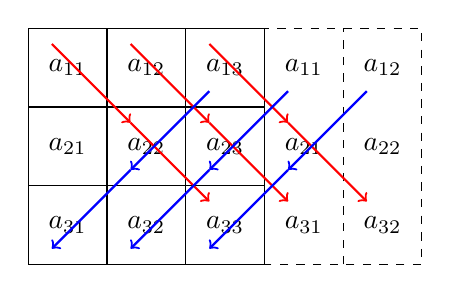
\begin{tikzpicture}
                % グリッドの作成
                \draw (0,0) rectangle (3,3);
                \draw (1,0) -- (1,3);
                \draw (2,0) -- (2,3);
                \draw (0,1) -- (3,1);
                \draw (0,2) -- (3,2);
        
                % 右側に追加の列
                \draw[dashed] (3,0) rectangle (5,3);
                \draw[dashed] (4,0) -- (4,3);
        
                % 行列の要素
                \node at (0.5,2.5) {$a_{11}$};
                \node at (1.5,2.5) {$a_{12}$};
                \node at (2.5,2.5) {$a_{13}$};
                \node at (0.5,1.5) {$a_{21}$};
                \node at (1.5,1.5) {$a_{22}$};
                \node at (2.5,1.5) {$a_{23}$};
                \node at (0.5,0.5) {$a_{31}$};
                \node at (1.5,0.5) {$a_{32}$};
                \node at (2.5,0.5) {$a_{33}$};
        
                % 右側の複製部分
                \node at (3.5,2.5) {$a_{11}$};
                \node at (4.5,2.5) {$a_{12}$};
                \node at (3.5,1.5) {$a_{21}$};
                \node at (4.5,1.5) {$a_{22}$};
                \node at (3.5,0.5) {$a_{31}$};
                \node at (4.5,0.5) {$a_{32}$};
        
                % 正の対角線(赤色)
                \draw[red, thick, ->] (0.3,2.8) -- (1.3,1.8);
                \draw[red, thick, ->] (1.3,1.8) -- (2.3,0.8);
        
                \draw[red, thick, ->] (1.3,2.8) -- (2.3,1.8);
                \draw[red, thick, ->] (2.3,1.8) -- (3.3,0.8);
        
                \draw[red, thick, ->] (2.3,2.8) -- (3.3,1.8);
                \draw[red, thick, ->] (3.3,1.8) -- (4.3,0.8);
        
                % 負の対角線(青色)
                \draw[blue, thick, ->] (2.3,2.2) -- (1.3,1.2);
                \draw[blue, thick, ->] (1.3,1.2) -- (0.3,0.2);
        
                \draw[blue, thick, ->] (3.3,2.2) -- (2.3,1.2);
                \draw[blue, thick, ->] (2.3,1.2) -- (1.3,0.2);
        
                \draw[blue, thick, ->] (4.3,2.2) -- (3.3,1.2);
                \draw[blue, thick, ->] (3.3,1.2) -- (2.3,0.2);
            \end{tikzpicture}
            \caption{サラスの方法}
        \end{figure}
        この図において, 赤線を通る文字の積は$+$, 青線を通る文字の積は$-$の符号をつけてすべて足し合わせればよい. 
        これは2次の場合でも同様にできるが, 4次以上の場合はできない.

        通常, 4次以上の行列式は式変形を繰り返すことで次数の小さい行列式で表し, 計算していくことで求める. 
        まずは, 行列式の基本的な性質についてみていこう. 基本的なのは, 次の二つである.
        \begin{align}
            \begin{vmatrix}
                a_{11} & a_{12} & \cdots & a_{1n} \\
                \hdotsfor{4}\\
                a_{k1}+a_{k1}' & a_{k2}+a_{k2}' & \cdots & a_{kn}+a_{kn}' \\
                \hdotsfor{4}\\
                a_{n1} & a_{n2} & \cdots & a_{nn}
            \end{vmatrix}
            &=\begin{vmatrix}
                a_{11} & a_{12} & \cdots & a_{1n} \\
                \hdotsfor{4}\\
                a_{k1} & a_{k2} & \cdots & a_{kn} \\
                \hdotsfor{4}\\
                a_{n1} & a_{n2} & \cdots & a_{nn}
            \end{vmatrix}
            +\begin{vmatrix}
                a_{11} & a_{12} & \cdots & a_{1n} \\
                \hdotsfor{4}\\
                a_{k1}' & a_{k2}' & \cdots & a_{kn}' \\
                \hdotsfor{4}\\
                a_{n1} & a_{n2} & \cdots & a_{nn}
            \end{vmatrix}
            \label{eq:線形代数:行列式の和}\\
            \begin{vmatrix}
                a_{11} & a_{12} & \cdots & a_{1n} \\
                \hdotsfor{4}\\
                ca_{k1} & ca_{k2} & \cdots & ca_{kn} \\
                \hdotsfor{4}\\
                a_{n1} & a_{n2} & \cdots & a_{nn}
            \end{vmatrix}
            &=c\begin{vmatrix}
                a_{11} & a_{12} & \cdots & a_{1n} \\
                \hdotsfor{4}\\
                a_{k1} & a_{k2} & \cdots & a_{kn} \\
                \hdotsfor{4}\\
                a_{n1} & a_{n2} & \cdots & a_{nn}
            \end{vmatrix}
            \label{eq:線形代数:行列式のスカラー倍}
        \end{align}
        これらは, 行列式の列に関する\textbf{多重線形性}\index{たじゅうせんけいせい@多重線形性}という. 証明は定義\eqref{eq:線形代数:行列式の定義}から明らかであろう.
        また, これらの性質は行に関しても言える. それを保証するのが, 次の転置行列に関する定理である.
        \begin{screen}
            正方行列$A$について$|A|=|{}^t\!A|$
        \end{screen}
        \begin{proof}
            $A=(a_{ij}),{}^t\!A=(b_{ij})$とおく. このとき, $b_{ij}=a_{ji}$に注意する.
            \begin{equation*}
                |{}^t\!A|=\sum_{\sigma} \sign\sigma\cdot b_{1\sigma(1)}b_{2\sigma(2)}\cdots b_{n\sigma(n)}=\sum_{\sigma} \sign\sigma\cdot a_{\sigma(1)1}a_{\sigma(2)2}\cdots a_{\sigma(n)n}
            \end{equation*}
            であり, $\sigma(1),\sigma(2),\cdots,\sigma(n)$の順番を$1,2,\cdots,n$となるように掛ける順番を変える.  
            このとき, $\sigma$は全単射だから, 逆写像$\sigma^{-1}$が存在して, しかも全ての$\sigma$について和を取る場合と全ての$\sigma^{-1}$について和を取る場合とで取りうる置換は変わらず, $\sign\sigma=\sign\sigma^{-1}$であるから.
            次のようになる.
            \begin{equation*}
                \sum_{\sigma^{-1}} \sign\sigma^{-1}\cdot a_{1\sigma^{-1}(1)}a_{2\sigma^{-1}(2)}\cdots a_{n\sigma^{-1}(n)}=\sum_{\sigma} \sign\sigma\cdot a_{1\sigma(1)}a_{2\sigma(2)}\cdots a_{n\sigma(n)}=|A|
            \end{equation*}
            以上より$|A|=|{}^t\!A|$が示された.
        \end{proof}
        \clearpage
        次の公式は, 証明は簡単であるが, 行列式の計算で重宝する.
        \begin{equation}
            \begin{vmatrix}
                a_{11} & a_{12} & \cdots & a_{1n}\\
                0 & a_{22} & \cdots & a_{2n}\\
                \vdots & \hdotsfor{3}\\
                0 & a_{n2} & \cdots & a_{nn}
            \end{vmatrix}
            =a_{11}\begin{vmatrix}
                a_{22} & \cdots & a_{2n}\\
                \hdotsfor{3}\\
                a_{n2} & \cdots & a_{nn}
            \end{vmatrix} \label{eq:線形代数:行列式の簡単化}
        \end{equation}
        \begin{proof}
            左辺において, $\sigma(1)=1$以外の場合の置換の和は全て0である. $\sigma(1)=1$の場合, $\sigma(i)\quad(i=2,3,\dots,n)$の選び方は自由であるから
            \begin{equation*}
                (左辺)=\sum\sign\sigma\cdot a_{1\sigma(1)}a_{2\sigma(2)}\cdots a_{n\sigma(n)}=a_{11}\sum_{\sigma\mid\sigma(1)=1}\sign\sigma\cdot a_{2\sigma(2)}\cdots a_{n\sigma(n)}=(右辺)
            \end{equation*}
            したがって等式が成り立つ.
        \end{proof}
        当然\eqref{eq:線形代数:行列式の簡単化}は行についても成り立つ. 

        行列式には多重線形性とは別に, もうひとつ重要な性質がある. 行列式の2つの行または2つの列を交換すると, 符号が変わる. これを行(または列の)\textbf{交代性}\index{こうたいせい@交代性}という.
        この証明は簡単だから演習問題とする.\\

        行列式について述べるからには, 次の定理について触れなければならないだろう.
        \begin{screen}
            二つの$n$次正方行列$A,B$について$|AB|=|A||B|$
        \end{screen}
        \begin{proof}
            $A=(a_{ij}),B=(b_{ij})$とおく. このとき$AB=(\sum a_{ik}b_{kj})$である.
            \begin{align*}
                |AB|&=\sum_{\sigma}\sign\sigma\cdot \left(\sum_{k_1}a_{1k_1}b_{k_1\sigma(1)}\right)\left(\sum_{k_2}a_{2k_2}b_{k_2\sigma(2)}\right)\cdots\left(\sum_{k_n}a_{nk_n}b_{k_n\sigma(n)}\right)\\
                &=\sum_{\sigma}\sign\sigma\cdot \sum_{k_1,k_2,\dots,k_n}a_{1k_1}b_{k_1\sigma(1)}a_{2k_2}b_{k_2\sigma(2)}\cdots a_{nk_n}b_{k_n\sigma(n)}
            \end{align*}
            ところで, 数字$k_1\sigma(1),k_2\sigma(2),\dots,k_n\sigma(n)$を並べ替えたものは, 和を取った時に打ち消しあう. したがって, $\sum$内の$k_1,k_2,\dots,k_n$は全て異なる値を取っていなければならない.
            \footnote{$\sigma$の各値はそれぞれ互いに違う. 仮に$k_i=k_j(i\neq j)$であるとき, $\sigma(i)$と$\sigma(j)$だけ値を入れ替えた置換も存在するから, このときちょうど打ち消しあってしまう.}
            すなわち, $\sum\limits_{k_1,k_2,\dots,k_n}$はある置換$k$の取りうる全ての和$\sum\limits_{k}$と考えてよい.\footnote{以下の$k_i$は本来は$k(i)$と書くべきだが, 紙面の都合上$k_i$のまま書いている.}  よって
            \begin{equation*}
                \sum_{\sigma}\sum_{k}\sign\sigma\cdot a_{1k_1}b_{k_1\sigma(1)}a_{2k_2}b_{k_2\sigma(2)}\cdots a_{nk_n}b_{k_n\sigma(n)}=\sum_{k}a_{1k_1}a_{2k_2}\cdots a_{nk_n}\left(\sum_{\sigma}\sign \sigma\cdot b_{k_1\sigma(1)}b_{k_2\sigma(2)}\cdots b_{k_n\sigma(n)}\right)
            \end{equation*}
            右辺の$(\hspace{1mm})$内は, $|B|$の行を並び変えたものである. このとき, 置換$k$が偶置換であるか奇置換であるかによって, $(\hspace{1mm})$の符号が変わる(行の交代性). これより
            \begin{equation*}
                \sum_{k}a_{1k_1}a_{2k_2}\cdots a_{nk_n}\sign k|B|=|B|\sum_{k}\sign k\cdot a_{1k_1}a_{2k_2}\cdots a_{nk_n}=|A||B|
            \end{equation*} 
            以上より$|AB|=|A||B|$が示された.
        \end{proof}
        \clearpage
        行列式を用いて, 二つの平面ベクトルが作る面の面積を求めることができる.\footnote{これはベクトル解析で述べる外積を用いればより一般に求められる.} 二つのベクトル$\bm{a},\bm{b}$のなす角度をなす角度を$\theta$とすると, 
        作られる面は平行四辺形であるから, $S=\left||\bm{a}||\bm{b}|\sin\theta\right|$となる. 絶対値記号は都合が悪いから, 両辺を二乗すると,
        $S^2=|\bm{a}|^2|\bm{b}|^2\sin^2\theta=|\bm{a}^2||\bm{b}^2|(1-\cos^2\theta)$となる.
        ここで, $\bm{a}=(a_x,a_y),\bm{b}=(b_x,b_y)$と置くと
        \begin{align*}
            S^2&=(a_x^2+a_y^2)(b_x^2+b_y^2)\left(1-\frac{(a_xb_x+a_yb_y)^2}{(a_x^2+a_y^2)(b_x^2+b_y^2)}\right)=(a_x^2+a_y^2)(b_x^2+b_y^2)-(a_xb_x+a_yb_y)^2\\
            &=a_x^2b_y^2+a_y^2b_x^2-2a_xa_yb_xb_y=(a_xb_y-a_yb_x)^2
        \end{align*}
        となるから, 求める面積は
        \begin{equation}
            S=|a_xb_y-a_yb_x|=\left|\det\begin{pmatrix}
                a_x & a_y \\ b_x & b_y
            \end{pmatrix}\right| \label{eq:線形代数:二つのベクトルがなす面の面積}
        \end{equation}
        となる. つまり, $\bm{a},\bm{b}$の二つのベクトルがなす面の面積は, 二つのベクトルの成分を横に並べてできる行列の行列式の絶対値に等しい.
        \begin{figure}[h]
            \centering
            \begin{tikzpicture}
                \fill[gray!20] (0,0) coordinate (O) -- (2,0.5) coordinate(A) -- (2.5,2.5) -- (0.5,2) coordinate (B) -- (0,0);
                \draw[-latex] (0,0) -- (2,0.5);
                \draw[-latex] (0,0) -- (0.5,2);
                \node[below] at (1,0.25) {$\bm{a}$};
                \node[left] at (0.25,1) {$\bm{b}$};
                \draw pic["$\theta$", draw, <->, font=\footnotesize, angle eccentricity=1.2, angle
                radius=1cm] {angle=A--O--B};
            \end{tikzpicture}
            \caption{二つのベクトルがなす面}
        \end{figure}
    \clearpage
    \subsection{余因子展開}
        最後に, 余因子展開について述べよう. $n$次正方行列$A$の第$i$行, 第$j$列を除いてできる$n-1$次の行列式を, $a_{ij}$に対する\textbf{小行列式}\index{しょうぎょうれつしき@小行列式}といい, 
        これに符号$(-1)^{i+j}$をかけたものを$A$の$a_{ij}$に対する\textbf{余因子}\index{よいんし@余因子}という. 以降余因子は$\tilde{A}_{ij}$と書くことにする.\\

        余因子を用いて行列式を展開することができる. $A$を$n$次の正方行列とすれば
        \begin{align}
            |A|&=a_{1j}\tilde{A}_{1j}+a_{2j}\tilde{A}_{2j}+\cdots+a_{nj}\tilde{A}_{nj}\quad &(j=1,2,\dots,n) \label{eq:線形代数:列に関する余因子展開}\\
            |A|&=a_{i1}\tilde{A}_{i1}+a_{i2}\tilde{A}_{i2}+\cdots+a_{in}\tilde{A}_{in}\quad &(i=1,2,\dots,n) \label{eq:線形代数:行に関する余因子展開}
        \end{align}
        が成り立つ. これらはそれぞれ第$j$列, 第$i$行に関する\textbf{余因子展開}\index{よいんしてんかい@余因子展開}という.
        \begin{proof}
            \eqref{eq:線形代数:列に関する余因子展開}を証明すれば, 転置行列を取って\eqref{eq:線形代数:行に関する余因子展開}も示される. よって, \eqref{eq:線形代数:列に関する余因子展開}のみ示す.
            $j=1$の場合をまず示そう. 行列の多重線形性\eqref{eq:線形代数:行列式の和}より
            \begin{equation*}
                |A|=
                \begin{vmatrix}
                    a_{11} & a_{12} & \cdots & a_{1n}\\
                    0 & a_{22} & \cdots & a_{2n}\\
                    \hdotsfor{4}\\
                    0 & a_{n2} & \cdots & a_{nn}
                \end{vmatrix}
                +\begin{vmatrix}
                    0 & a_{12} & \cdots & a_{1n}\\
                    a_{21} & a_{22} & \cdots & a_{2n}\\
                    \hdotsfor{4}\\
                    0 & a_{n2} & \cdots & a_{nn}
                \end{vmatrix}
                +\cdots
                +\begin{vmatrix}
                    0 & a_{12} & \cdots & a_{1n}\\
                    0 & a_{22} & \cdots & a_{2n}\\
                    \hdotsfor{4}\\
                    a_{n1} & a_{n2} & \cdots & a_{nn}
                \end{vmatrix}
            \end{equation*}
            ここで, 各行列式の$1$列目のうち, $0$でない要素$a_{m1}$を$(1,1)$成分に移動させると, $(-1)^{m-1}$の符号をかければよいから
            \begin{equation*}
                \begin{vmatrix}
                    a_{11} & a_{12} & \cdots & a_{1n}\\
                    0 & a_{22} & \cdots & a_{2n}\\
                    \hdotsfor{4}\\
                    0 & a_{n2} & \cdots & a_{nn}
                \end{vmatrix}
                -\begin{vmatrix}
                    a_{21} & a_{22} & \cdots & a_{2n}\\
                    0 & a_{12} & \cdots & a_{1n}\\
                    \hdotsfor{4}\\
                    0 & a_{n2} & \cdots & a_{nn}
                \end{vmatrix}
                +\cdots
                +(-1)^{n-1}\begin{vmatrix}
                    a_{n1} & a_{n2} & \cdots & a_{nn}\\
                    0 & a_{12} & \cdots & a_{1n}\\
                    \hdotsfor{4}\\
                    0 & a_{(n-1)2} & \cdots & a_{(n-1)n}\\
                \end{vmatrix}
            \end{equation*}
            ここで, \eqref{eq:線形代数:行列式の簡単化}を用いれば
            \begin{equation*}
                a_{11}\begin{vmatrix}
                    a_{22} & \cdots & a_{2n}\\
                    \hdotsfor{3}\\
                    a_{n2} & \cdots & a_{nn}
                \end{vmatrix}
                -a_{21}\begin{vmatrix}
                    a_{12} & \cdots & a_{1n}\\
                    \hdotsfor{3}\\
                    a_{n2} & \cdots & a_{nn}
                \end{vmatrix}
                +\cdots
                +(-1)^{n-1}a_{n1}\begin{vmatrix}
                    a_{12} & \cdots & a_{1n}\\
                    \hdotsfor{3}\\
                    a_{(n-1)2} & \cdots & a_{(n-1)n}\\
                \end{vmatrix}
            \end{equation*}
            よって, 次が得られる.
            \begin{equation*}
                |A|=a_{11}\tilde{A}_{11}+a_{21}\tilde{A}_{21} +\cdots+ a_{n1}\tilde{A}_{n1}
            \end{equation*}
            一般の$j$列については, $j$列の要素を一番左に持っていき, 先ほどと同様行列の多重線形性から変形を行えばよい.
        \end{proof}
        余因子は, それ自身行列の計算において大切であるが, 逆行列を求める際にも用いることができる. そのための準備をしよう. 余因子$\tilde{A}_{\bm{j}\bm{i}}$(添え字に注意)を
        $(i,j)$成分に持つ行列$\tilde{A}$を考える. これを$A$の\textbf{余因子行列}\index{よいんしぎょうれつ@余因子行列}という.
        \begin{equation}
            \tilde{A}
            =\begin{pmatrix}
                \tilde{A}_{11} & \tilde{A}_{21} & \cdots & \tilde{A}_{n1} \\
                \tilde{A}_{12} & \tilde{A}_{22} & \cdots & \tilde{A}_{n2} \\
                \hdotsfor{4}\\
                \tilde{A}_{1n} & \tilde{A}_{2n} & \cdots & \tilde{A}_{nn}    
            \end{pmatrix} \label{eq:線形代数:余因子行列の定義}
        \end{equation}
        ここで, 行列$A$と余因子行列$\tilde{A}$の積$A\tilde{A}$を考えてみる. すぐわかるように, 対角成分は$|A|$である. 
        それ以外の成分は, `逆'余因子展開をして$n$次の行列式に直せば, どこかの行がまったく同一になる.\footnote{$(l,m)$成分は$a_{l1}\tilde{A}_{m1}+\cdots+a_{ln}\tilde{A}_{mn}$であり, これを`逆'余因子展開した時の$m$行目は$a_{l1},a_{l2},\dots,a_{ln}$であるが,
        $m\neq l$のときは, この行列式の$l$行目も$a_{l1},a_{l2},\dots,a_{ln}$であり, 同一な行が現れる.}
            \eqref{eq:線形代数:行列式の和}および\eqref{eq:線形代数:行列式の簡単化}
        を用いれば, 2つの行が等しい行列式の値が0であることがわかり, これは$\tilde{A}A$でも同様のことが言えるから, 結局, 次のようになる.
        \begin{equation}
            A\tilde{A}=\tilde{A}A
            =\begin{pmatrix}
            |A| & 0 & \cdots & 0\\
            0 & |A| & \cdots & 0\\
            \hdotsfor{4}\\
            0 & 0 & \cdots & |A|    
            \end{pmatrix}
            =|A|E \label{eq:線形代数:余因子行列との積}
        \end{equation}
        ここから, $|A|\neq 0$であれば, $A$の逆行列は$\frac{1}{|A|}\tilde{A}$であることがわかる. また, $A$が正則であれば, $1=|E|=|AA^{-1}|=|A||A^{-1}|$であるから, $|A|\neq 0$である. 
        以上をまとめると, 次の結果が得られた.
        \begin{screen}
            正方行列$A$について, $A$が正則である必要十分条件は$|A|\neq 0$であり, このとき逆行列は
            \begin{equation}
                A^{-1}=\frac{1}{|A|}\tilde{A} \label{eq:線形代数:逆行列の公式}
            \end{equation}
            で与えられる.
        \end{screen}

        例えば, 2次正方行列の逆行列は\eqref{eq:線形代数:2次の正方行列の逆行列}で与えていたが, これも\eqref{eq:線形代数:逆行列の公式}から導出できる. $A=\begin{pmatrix}a & b \\ c & d\end{pmatrix}$
        であるとき, 各余因子は
        \begin{align*}
            \tilde{A}_{11} &= d \quad &&\tilde{A}_{12} = -c\\
            \tilde{A}_{21} &= -b\quad &&\tilde{A}_{22} =a 
        \end{align*}
        であり, $|A|=ad-bc$であるから, 逆行列は$ad-bc\neq 0$
        \begin{equation*}
            A^{-1}
            =\frac{1}{|A|}\begin{pmatrix}
                \tilde{A}_{11} & \tilde{A}_{21}\\
                \tilde{A}_{12} & \tilde{A}_{22}
            \end{pmatrix}
            =\frac{1}{ad-bc}\begin{pmatrix}
                d & -b \\ -c & a
            \end{pmatrix}
        \end{equation*}
        と求まる.
\clearpage
\basicquestion 以下の問いに答えよ。

    \subsubsection*{問1} ベクトルの計算問題を解いてみよう. $\bm{a}=(1,2),\bm{b}=(3,5),\bm{c}=(-3,-5)$とする.\\
        $(1)\bm{a}+\bm{b}$\hspace{1mm}
        $(2)\bm{a}-\bm{c}$\hspace{1mm}
        $(3)\bm{a}\cdot\bm{b}$\hspace{1mm}
        $(4)(\bm{a}+\bm{c})^2$\hspace{1mm}
        $(5)(\bm{a}\cdot\bm{c})\bm{b}-(\bm{a}\cdot\bm{b})\bm{c}$\hspace{1mm}
        $(6)$ベクトル$\bm{p}=(8,15)$を正規化せよ.

    \subsubsection*{問2} 次の二つのベクトルのなす角度を求めよ.\\
        $(1)\bm{a}=(2,1),\bm{b}=(-1,-2)$\hspace{1mm}
        $(2)\bm{a}=(\sqrt{3},-2),\bm{b}=(\sqrt{3},5)$

    \subsubsection*{問3}$A=\begin{pmatrix}4 & 6\\2 & 3\end{pmatrix},B=\begin{pmatrix}3 & -6\\-4 & 8\end{pmatrix}$であるとき, $A+B,2A-3B,AB,BA$を求めよ.
    
    \subsubsection*{問4}$f$が線形変換である, つまり\eqref{eq:線形代数:線形変換の定義}であることと, $f$が\eqref{eq:線形代数:線形変換の条件1},\eqref{eq:線形代数:線形変換の条件2}を満たすことは同値であることを, 2次元の場合で証明せよ.

    \subsubsection*{問5}次の行列式を計算せよ.\\
        $(1)\begin{vmatrix}3 & 2 \\ 4 & 1\end{vmatrix}$\hspace{1mm}
        $(2)\begin{vmatrix}2 & -1\\ 3 & 1\end{vmatrix}$\hspace{1mm}
        $(3)\begin{vmatrix}2 & -1 & 6 \\ 5 & 0 & 1 \\ 3 & 2 & 4\end{vmatrix}$\hspace{1mm}
        $(4)\begin{vmatrix}1 & 2 & 3 \\ 4 & 5 & 6 \\ 7 & 8 & 9\end{vmatrix}$\hspace{1mm}
        $(5)\begin{vmatrix}0 & 2 & 0 & 0 \\ 3 & 5 & 0 & 0 \\ 0 & 0 & \pi &4 \\ 0 & 0 & 2\pi & 3\end{vmatrix}$\hspace{1mm}
        $(6)\begin{vmatrix}3 & -2 & 5 & 1 \\ 1 & 3 & 2 & 5 \\ 2 & -5 & -1 & 4 \\ -3 & 2 & 3 & 2\end{vmatrix}$
    \subsubsection*{問6}3次正方行列$A$について$|A|=3$であるとき$|5A|$を求めよ.

    \subsubsection*{問7}行列式の交代性を証明せよ.

    \subsubsection*{問8}$A=\begin{pmatrix}
        3 & 1 & 2\\
        3 & 2 & 1\\
        4 & 2 & 3
    \end{pmatrix}$が正則かどうかを調べ, 正則であれば逆行列を求めよ.
    \vspace{-0.5cm}

    \subsubsection*{問9} 2次の正方行列$A=\begin{pmatrix}1 & 2\\-1 & 4\end{pmatrix}$について, $A\bm{x}=\lambda\bm{x}$を満たす実数$\lambda$および列ベクトル$\bm{x}$を求めよ. このときの$\lambda$を$A$の
    \textbf{固有値}\index{こゆうち@固有値}, $\bm{x}$を固有値$\lambda$に対する\textbf{固有ベクトル}\index{こゆうべくとる@固有ベクトル}という. 
\clearpage
\section{偏微分}
    多変数関数をまず具体例で挙げ, その後偏微分について解説する.二変数関数のTaylor展開及び積分記号下の微分まで述べる.
    \subsection{多変数関数}
        これまで, 関数といえば一変数関数のことを指していた. しかし実際には一つのパラメータのみで表せる現象などは少ない. たいていの場合は, 複数のパラメータを持っているものである.
        例えば, 物体の平面運動を考えるときは$x,y$の二つの編すが必要である. 理想気体の状態方程式に至っては, $PV=nRT$であるから, 例えば温度$T$に着目すれば$P,V,n$の三つの変数が
        必要である.\footnote{$R$は気体定数であるから, これは変数ではない.}

        このような複数の独立変数に対して, 一つの従属変数が決まるとき, この関数を多変数関数という. 独立変数を$x_1,x_2,\dots,x_n$, 従属変数を$y$, 多変数関数を$f$とするとき, $y=f(x_1,x_2,\dots,x_n)$
        とかく.\footnote{お気づきの方も多いように, 本来であれば, $y=f((x_1,x_2,\dots,x_n))$と書くべきであるが, やはりこれも慣習なのだろう.}
        以後, 主に二変数を扱っていくから, 独立変数に$x,y$, 従属変数に$z$を用いることにする.

        多変数関数の例を見てみよう. もっとも簡単な例は, $z=x+y$である. これは平面を表す. 一般に, $a,b,c$を定数として, $z=ax+by+c$は平面を表す.
        半径1の球の方程式は, $x^2+y^2+z^2=1$である. これを変形して$z=\sqrt{1-x^2-y^2}$は, 球の上半分を表す.
        二変数関数のグラフは三次元空間上に描かれるから, これを描くのは困難である. 適当なグラフ描画ソフトで描画してみることをお勧めする. もちろん, 三変数以上の場合は絵を描くことすら困難である.

        \begin{figure}[h]
            \centering
            \begin{minipage}[t]{0.45\textwidth}
                \centering
                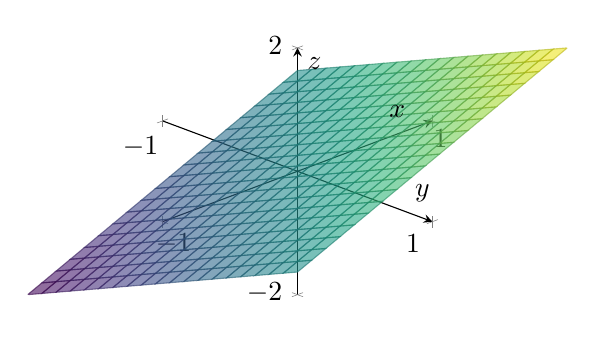
\begin{tikzpicture}
                    \begin{axis}[
                        view={45}{-30}, % 視点の設定
                        axis lines=center, % 軸を中央に配置
                        xlabel={$x$}, ylabel={$y$}, zlabel={$z$},
                        domain=-1:1, y domain=-1:1, % 定義域の設定
                        samples=20, % グリッドの細かさ
                        enlargelimits=false, % 領域の拡大を防ぐ
                        colormap/viridis % 色設定
                    ]

                        \addplot3[surf, opacity=0.6] 
                            {x+y};
                    \end{axis}
                \end{tikzpicture}
                \subcaption{平面$z=x+y$}
            \end{minipage}
            \begin{minipage}[t]{0.45\textwidth}
                \centering
                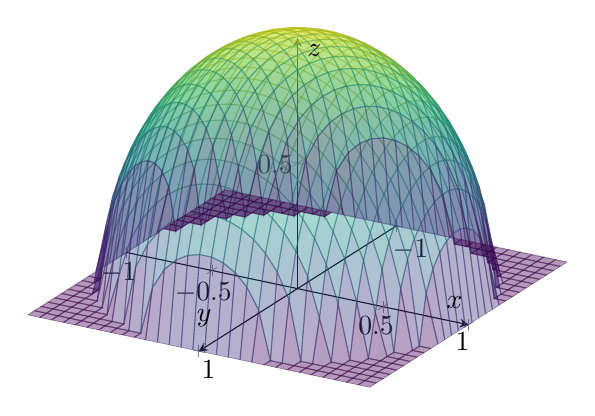
\begin{tikzpicture}
                    \begin{axis}[
                        view={-30}{-30}, % 視点の設定
                        axis lines=center, % 軸を中央に配置
                        xlabel={$x$}, ylabel={$y$}, zlabel={$z$},
                        domain=-1:1, y domain=-1:1, % 定義域の設定
                        samples=30, % グリッドの細かさ
                        enlargelimits=false, % 領域の拡大を防ぐ
                        colormap/viridis % 色設定
                    ]
                
                        \addplot3[surf, opacity=0.4] 
                            {sqrt(max(0,1 - x^2 - y^2))};
                    \end{axis}
                \end{tikzpicture}
                \subcaption{球面$z=\sqrt{1-x^2-y^2}$}
            \end{minipage}
            \caption{多変数関数のグラフの例}
        \end{figure}
    \clearpage
    \subsection{偏微分}
        さっそく, この節の題にもなっている偏微分について述べようと思う. 二変数関数$z=f(x,y)$に対して, 次の極限を考える.
        \begin{equation}
            \frac{\partial z}{\partial x} =\lim_{\Delta x\to 0}\frac{f(x+\Delta x,y)-f(x,y)}{\Delta x} \label{eq:偏微分:xについて偏微分} 
        \end{equation}
        これは, 複数の変数を持つ関数において, ただ一つの変数のみを変化させて, その変数に関して微分している. この場合は, $x$について変化させて微分しているから, 
        この極限が存在するとき, $x$について\textbf{偏微分可能}\index{へんびぶんかのう@偏微分可能}であるといい, このときの微分を\textbf{偏微分}\index{へんびぶん@偏微分}という.
        同様に, $y$について偏微分するとは
        \begin{equation}
            \frac{\partial z}{\partial y} =\lim_{\Delta y\to 0}\frac{f(x,y+\Delta y)-f(x,y)}{\Delta y} \label{eq:偏微分:yについて偏微分} 
        \end{equation}
        ということになる. これらは\textbf{偏導関数}\index{へんどうかんすう@偏導関数}とよばれる.

        偏導関数の記法は様々なものがある.
        \begin{equation}
            \frac{\partial z}{\partial x},\quad \frac{\partial f}{\partial x},\quad f_x,\quad z_x,\quad D_x f,\quad \partial_x f,\quad\cdots
        \end{equation}
        これらはそれぞれ長所短所があるが, このノート中では特に拘泥せず使っていくことにする. ちなみに, $\partial$は$d$の変形であり, パーシャルやデル, または単にディーと読む.

        例を挙げよう. $z=x+y$において, 偏導関数は$z_x=1,z_y=1$である. また, $z=\sqrt{1-x^2-y^2}$の偏導関数は$z_x=-x/\sqrt{1-x^2-y^2},z_y=-y/\sqrt{1-x^2-y^2}$となる.
        偏微分する変数以外は定数とみなすことがポイントである.
        
        次に, 高階微分について考えてみよう. $f_x,f_y$はともに$x,y$の関数であるから, これらも偏微分することができるはずである. こうして得られる偏導関数を二階偏導関数という.
        偏導関数には次の4種がある.
        \begin{equation*}
            f_{xx},\quad f_{xy},\quad f_{yx},\quad f_{yy} 
        \end{equation*}
        またこれらは次のようにも書かれる.
        \begin{equation*}
            \frac{\partial^2 f}{\partial x^2},\quad \frac{\partial^2 f}{\partial x\partial y},\quad \frac{\partial^2 f}{\partial y\partial x},\quad \frac{\partial^2 f}{\partial y^2}
        \end{equation*}
        先ほど例で挙げた関数について, 二階偏導関数を計算してみる. $z=x+y$の場合, $z_{xx}=0,z_{xy}=0,z_{yx}=0,z_{yy}=0$である. また, $z=\sqrt{1-x^2-y^2}$の場合, $z_{xx}=(y^2-1)/(1-x^2-y^2)^{3/2},z_{xy}=-xy/(1-x^2-y^2)^{3/2},z_{yx}=-xy/(1-x^2-y^2)^{3/2},z_{yy}=(x^2-1)/(1-x^2-y^2)^{3/2}$となる.
        この例では$z_{xy}=z_{yx}$が成り立つことがわかる. これは偶然ではない. 実は, 次が成り立つ.
        \begin{screen}
            多変数関数$f$に対して, $f_{xy},f_{yx}$が連続ならば
            \begin{equation}
                f_{xy}=f_{yx} \label{eq:偏微分:偏微分の交換}
            \end{equation}
            が成り立つ.
        \end{screen}
        しかも, これはより高階な場合でも同様に成り立つ. つまり, それぞれの偏導関数が連続ならば, それらの偏微分の順序は交換できるのだ.

        しかしながら, 我々はまだ多変数関数の連続の定義に触れていなかった. そこで, 多変数の場合の極限と連続について述べておこう.
        まずは, 極限についてである. 二変数関数$f(x,y)$の定義域内において, 点$P(x,y)$がこの領域内を移動し, 限りなくある点$A(a,b)$\footnote{この点は定義域内になくてもよい. 正確には, 定義域の閉包(領域と境界の和集合)上の点であればよい.}に近づくとき, 
        それに伴い$f(P)=f(x,y)$が限りなく一定の値$\alpha$に近づくならば, $f(x,y)$には\textbf{極限}が存在し, その極限値は$\alpha$であるといい,
        \begin{equation}
            \lim_{(x,y)\rightarrow(a,b)}f(x,y)=\alpha \label{eq:偏微分:二変数関数の極限}
        \end{equation}
        とかく. $\varepsilon-\delta$風に書けば, $f$の定義域を$D$として
        \begin{equation}
            {}^\forall \varepsilon>0,{}^\exists \delta>0,{}^\forall(x,y)\in D \left[0<|x-a|<\delta,0<|y-b|<\delta\Rightarrow |f(x,y)-\alpha|<\varepsilon\right] \label{eq:偏微分:二変数関数の極限の定義}
        \end{equation}
        であろうか. 注意しなければならないのは, $P\rightarrow A$の近づき方が\underline{どんな近づき方であっても}, 同一の極限値に近づくという点である.
        例えば, 
        \begin{equation*}
            f(x,y)=\frac{x}{x+y}
        \end{equation*}
        の原点への近づき方を考えている. 例えば, x軸に沿って近づける場合
        \begin{equation*}
            \lim_{(x,0)\rightarrow (0,0)}f(x,y)=\lim_{x\rightarrow 0}f(x,0)=\lim_{x\rightarrow 0}\frac{x}{x}=1
        \end{equation*}
        であるが, y軸に沿って近づける場合は
        \begin{equation*}
            \lim_{(0,y)\rightarrow (0,0)}f(x,y)=\lim_{y\rightarrow 0}f(0,y)=\lim_{y\rightarrow 0}0=0
        \end{equation*}
        となるから, 近づき方によって極限が異なる. この場合は極限値は存在しないということになる.

        さて, 次は連続について述べよう. これも一変数の場合と同様である. 極限のときの記号をそのまま用いることにする. このとき, $f(x,y)$が定義域内の点$A(a,b)$で\textbf{連続}であるとは, 次の三つの条件を満たすことである.
        \begin{enumerate}
            \item $f(a,b)$が定義されている.
            \item $\lim\limits_{(x,y)\to(a,b)}f(x,y)$が存在する.
            \item $f(a,b)=\lim\limits_{(x,y)\to(a,b)}f(x,y)$である.
        \end{enumerate}
        先ほど例で上がった関数$f(x,y)$は明らかに原点で連続でない. 一方, 次のような関数ではどうだろう.
        \begin{equation*}
            f(x,y)=\left\{\begin{array}{cc}
                \displaystyle\frac{x^3+y^3}{x^2+y^2} & ((x,y)\neq (0,0))\\
                1 & ((x,y)=(0,0))
            \end{array}\right.
        \end{equation*}
        実は, この場合でも原点で連続でない. $x=r\cos\theta,y=r\sin\theta$と置くと, 極限は$r\to 0$となる. よって
        \begin{equation*}
            \lim_{(x,y)\to(0,0)}f(x,y)=\lim_{r\to\infty}\frac{r^3(\cos^3\theta+\sin^2\theta)}{r^2}=\lim_{r\to 0}r(\cos^3\theta+\sin^3\theta)=0
        \end{equation*}
        となるから, 極限は存在して$0$である\footnote{厳密には, $\varepsilon-\delta$で確かめる必要がある.}が, $f(0,0)=1$であるからこれは連続でない. しかし, $f(0,0)=0$と定義しなおせば連続になる.\\

        ここでは二変数の場合についてのみのべたが, 三変数以上でも同様であることを付記しておく.
    \clearpage
    \subsection{全微分}
        ここでは, 全微分について述べる. 関数$z=f(z,y)$について, 点$P(x,y)$の近傍で考えてみよう. この点$P$より, $\Delta x,\Delta y$だけ動かしたとき, $z$の値はどれくらい変わるだろうか.
        この変化の量を$\Delta z$と置けば, これはそれぞれの差を取ればよいから, $\Delta z=f(x+\Delta x,y+\Delta y)-f(x,y)$となる. ところで, $\Delta z$は, もちろん$x,y$によって変わってくるわけであるが, $\Delta x,\Delta y$
        によっても変化するだろう. そこで, $\Delta z$が次のように書けたとする.
        \begin{equation}
            \Delta z = A(x,y)\Delta x+B(x,y)\Delta y+o(\rho) \label{eq:偏微分:Δzの式}
        \end{equation}
        ここで, $\rho = \sqrt{(\Delta x)^2+(\Delta y)^2}$であって, これは$P$と$(x+\Delta x,y+\Delta y)$との距離を表す.
        なお, $o(\rho)$は$\rho\to 0$で$o(\rho)\to 0$を表す.\footnote{これは所謂\textbf{Landauの記号}\index{Landauのきごう@Landauの記号}であって, 正確には$f(x),g(x)$について, $x\to 0$のとき$f(x)/g(x)\to 0$であることを$f(x)=o(g(x))$であると書くのである.}
        このとき, $z=f(x,y)$は点$P(x,y)$で\textbf{全微分可能}\index{ぜんびぶんかのう@全微分可能}, または単に微分可能であるという.

        全微分可能であるならば, 偏微分可能である. 実際, $\Delta y=0$とすれば, $\rho=|\Delta x|\to 0$のとき
        \begin{equation*}
            \frac{\Delta z}{\Delta x}=A(x,y)+\varepsilon|\Delta x|\to A(x,y)
        \end{equation*}
        となる. またこのとき, $A(x,y)=z_x$である. $\Delta x=0$の場合も同様で, このとき, $B(x,y)=z_y$となる. もちろん, $z=f(x,y)$が$x,y$について
        偏微分可能であっても, 全微分可能であるとは限らない. しかし, 次が成り立つ.
        \begin{screen}
            ある領域内で$z_{x}$と$z_{y}$が存在して(どちらか一方が)連続ならば, $z$はその領域内で全微分可能である.
        \end{screen}
        \begin{proof}
            $z_{x}$が連続であるとしよう. まず, $\Delta z$を次のように変形する.
            \begin{equation*}
                \Delta z = \left\{f(x+\Delta x,y+\Delta y)-f(x,y+\Delta y)\right\}+\left\{f(x,y+\Delta y)-f(x,y)\right\}
            \end{equation*}
            一項目は平均値の定理より
            \begin{equation*}
                f(x+\Delta x,y+\Delta y)-f(x,y+\Delta y)=\Delta xf_{x}(x+\theta\Delta x,y+\Delta y) \quad (0<\theta<1)
            \end{equation*}
            しかも, $z_{x}=f_x$は連続である. 連続であれば, $f_x(x+\theta\Delta x,y+\Delta y)=f_{x}(x,y)+\varepsilon$と書ける. ただし, $\Delta x\to 0,\Delta y\to 0$で$\varepsilon\to 0$である.
            \footnote{実際, $f_{x}$は連続であるから, $|f_{x}(x+\theta\Delta x,y+\Delta y)-f_{x}(x,y)|<\varepsilon$となるような$\delta>|\Delta x|,|\Delta y|$が存在する.}

            一方で, $z_y$が存在するから, 二項目は
            \begin{equation*}
                f(x,y+\Delta y)-f(x,y)=\Delta yf_y(x,y)+\Delta y\varepsilon'
            \end{equation*}
            とかいてよい. ただし, $\Delta y\to 0$で$\varepsilon'\to 0$である. 以上より, $\Delta z$は次のようになる.
            \begin{equation*}
                \Delta z= f_{x}(x,y)\Delta x +f_{y}(x,y)\Delta y + \Delta x \varepsilon+\Delta y\varepsilon'
            \end{equation*}
            ここで, $|\Delta x|\leq\rho,|\Delta y|\leq\rho$が成り立つ. つまり, $|\Delta x\varepsilon+\Delta y\varepsilon'|\leq |\Delta x\varepsilon|+|\Delta y\varepsilon'|\leq(|\varepsilon|+|\varepsilon'|)\rho$が成立する. 
            したがって, $\rho\to 0$で$\Delta x\varepsilon+\Delta y\varepsilon'\to 0$であるから, $z$は全微分可能である.
        \end{proof}
        \clearpage
        さて, $z$が微分可能であるとき, $P(x,y)$に十分近ければ, $\Delta z\sim f_x\Delta x+f_y\Delta y$である. そこで, 次のように\textbf{全微分}\index{ぜんびぶん@全微分}を定義しよう.
        \begin{equation}
            dz = \frac{\partial z}{\partial x}\Delta x + \frac{\partial z}{\partial y}\Delta y \label{eq:偏微分:全微分の定義}
        \end{equation}
        すぐにわかるように, $z=x$と置けば, $dx=\Delta x$, $z=y$と置けば, $dy=\Delta y$であるから, \eqref{eq:偏微分:全微分の定義}は次のようになる.
        \begin{equation}
            dz = \frac{\partial z}{\partial x}dx + \frac{\partial z}{\partial y}dy \label{eq:偏微分:全微分}
        \end{equation}
        これはあくまで$\Delta z$の一次近似であるが, 少し頭を柔らかくして, これを$z$の``微小変化''と捉えることにする. そうすることで, 今後の議論が簡単になるし, 直感的にわかりやすくなる.\\

        次に, $z=f(x,y)$の$(a,b)$における\textbf{接平面}\index{せつへいめん@接平面}を定義しよう. それは次のように定義される.
        \begin{equation}
            z-f(a,b)=f_{x}(a,b) (x-a) + f_{y}(a,b) (y-b) \label{eq:偏微分:接平面の定義}
        \end{equation}
        これは, $z=ax+by+c$の形であるから, 確かに平面を表す. また, $(a,b,f(a,b))$を通る平面でもある. 接平面は直感的には, 点$(a,b)$で$z=f(x,y)$と接する平面であるととらえることができる.
        つまり, 一変数関数における接線に相当するものが, 接平面となる. 

        $z=f(x,y)$が全微分可能であるとき, 接平面は存在する. また, $z=f(x,y)$に対して接平面が存在するとき, その点において全微分可能である. なぜなら, 接平面を$z=p(x,y)$と置けば
        \begin{equation*}
            \lim_{\rho \to 0}\{\Delta z - p(x,y)\} = 0
        \end{equation*}
        であるから, $\Delta z = p(x,y)+\varepsilon\rho\quad (\rho\to 0で\varepsilon\rho\to 0)$と表すことができ, $p(x,y)=f_{x}(a,b)(x-a)+f_{y}(a,b)(y-b)=f_{x}(a,b)\Delta x+f_{y}(a,b)\Delta y$であるから, 
        結局, $\Delta z$を\eqref{eq:偏微分:Δzの式}で書くことができる. 
    \clearpage
    \subsection{合成関数の微分}
        次は合成関数の微分について述べよう. 以下の議論ではすべて全微分\eqref{eq:偏微分:全微分}を用いる.\footnote{したがって, この議論では$f(x,y)$の全微分可能性は暗に仮定されているわけである.} もちろん従来通り増分と極限から導出することもできるが, 直感的に理解していきたい.

        まずは, $z=f(x,y)$で, $x,y$がともに変数$t$の関数$x=x(t),y=y(t)$であるとしよう. このとき, $x(t),y(t)$がともに$t$で微分可能であれば, 次が成り立つ.
        \begin{equation*}
            dx=\frac{dx}{dt}dt,\quad dy=\frac{dy}{dt}dt
        \end{equation*}
        よって, $dz$は
        \begin{equation*}
            dz = \frac{\partial z}{\partial z}dx+\frac{\partial z}{\partial y}dy=\left(\frac{\partial z}{\partial x}\frac{dx}{dt}+\frac{\partial z}{\partial y}\frac{dy}{dt}\right)dt
        \end{equation*}
        一方, $z$は$t$の関数とみなせるから
        \begin{equation*}
            dz=\frac{dz}{dt}dt
        \end{equation*}
        上記二つの式を比較して
        \begin{equation}
            \frac{dz}{dt}=\frac{\partial z}{\partial x}\frac{dx}{dt}+\frac{\partial z}{\partial y}\frac{dy}{dt} \label{eq:偏微分:合成関数の微分t}
        \end{equation}
        が得られる. \\

        今度は, $x=x(u,v),y=y(u,v)$であるとき, $x(u,v),y(u,v)$がともに\underline{全微分可能}\footnote{これは過剰な要請である. 実際は$x(u,v),y(u,v)$は$u,v$で偏微分可能であればよい.}であれば
        \begin{equation*}
            dx=\frac{\partial x}{\partial u}du+\frac{\partial x}{\partial v}dv,\quad dy=\frac{\partial y}{\partial u}du+\frac{\partial y}{\partial v}dv
        \end{equation*}
        よって, $dz$は
        \begin{equation*}
            dz=\left(\frac{\partial z}{\partial x}\frac{\partial x}{\partial u}+\frac{\partial z}{\partial y}\frac{\partial y}{\partial u}\right)du+\left(\frac{\partial z}{\partial y}\frac{\partial y}{\partial v}+\frac{\partial z}{\partial y}\frac{\partial y}{\partial v}\right)dv
        \end{equation*}
        一方, $z$は$u,v$の関数とみなせるから
        \begin{equation*}
            dx=\frac{\partial z}{\partial u}du+\frac{\partial z}{\partial v}dv
        \end{equation*}
        これより次の公式が得られる.
        \begin{align}
            \frac{\partial z}{\partial u}=\frac{\partial z}{\partial x}\frac{\partial x}{\partial u}+\frac{\partial z}{\partial y}\frac{\partial y}{\partial u} \label{eq:偏微分:合成関数の微分u}\\
            \frac{\partial z}{\partial v}=\frac{\partial z}{\partial y}\frac{\partial y}{\partial v}+\frac{\partial z}{\partial y}\frac{\partial y}{\partial v} \label{eq:偏微分:合成関数の微分v}
        \end{align}
        これらの公式も, もちろん多変数に拡張できる. 
        \clearpage
        ここで, 合成関数の微分の理解度を深めるために, 一つ例題を解いてみる. $z=f(x,y)$が$y/x$の関数である必要十分条件は
        \begin{equation*}
            x\frac{\partial z}{\partial x}+y\frac{\partial z}{\partial y}=0
        \end{equation*}
        であることを示そう. ただし, $f(x,y)$は全微分可能であるとする.\\

        まずは, 十分条件から示そう. このとき, $z=g(t),t=y/x$と表せる. 一変数の合成関数の微分法より
        \begin{equation*}
            \frac{\partial z}{\partial x}=\frac{dg}{dt}\frac{\partial t}{\partial x}=-\frac{y}{x^2}\frac{dg}{dt},\quad \frac{\partial z}{\partial y}=\frac{dg}{dt}\frac{\partial t}{\partial y}=\frac{1}{x}\frac{dg}{dt}
        \end{equation*}
        であるから
        \begin{equation*}
            x\frac{\partial z}{\partial x}+y\frac{\partial z}{\partial y}=0
        \end{equation*}
        となる.

        次に, 必要条件を示す. $z=h(u,v),u=x,v=y/x$とおく. このとき\eqref{eq:偏微分:合成関数の微分u},\eqref{eq:偏微分:合成関数の微分v}より, 次が成り立つ.
        \begin{align*}
            x\frac{\partial z}{\partial x}+y\frac{\partial z}{\partial y}&=x\frac{\partial h}{\partial u}\left(x,\frac{y}{x}\right)+x\frac{\partial h}{\partial v}\left(x,\frac{y}{x}\right)\cdot \left(-\frac{y}{x^2}\right)+xv\frac{\partial h}{\partial v}\left(x,\frac{y}{x}\right)\cdot \frac{1}{x}=x\frac{\partial h}{\partial u}\left(x,\frac{y}{x}\right)-\frac{y}{x}\frac{\partial h}{\partial v}\left(x,\frac{y}{x}\right)+v\frac{\partial h}{\partial v}\left(x,\frac{y}{x}\right)\\
            &=x\frac{\partial h}{\partial u}\left(x,\frac{y}{x}\right)=0
        \end{align*}
        よって, $h_u=0$であるから, $h(u,v)$は$u$に無関係. すなわち, $z=f(x,y)$は$y/x$のみの関数である.
        以上で証明完了.
    \clearpage
    \subsection{二変数関数のTaylorの定理}
        一変数関数のときには, 平均値の定理やTaylorの定理など, 微分法に関する様々な定理を述べた. これらの定理は微分法で重要な位置を占めている. 当然, 二変数の場合も考えたくなるのが人間の性というものであろう. 
        ここでは, 二変数関数の場合の平均値の定理と, Taylorの定理について述べていきたい.

        まずは, 平均値の定理である. これは一変数の場合の平均値の定理から導出することができる. 全微分可能である関数$z=f(x,y)$と定数$a,b,h,k$を用いて, 一変数関数$F(t)$を次のように定める.
        \footnote{このとき, $f$が$(a,b)$を含むある領域内で全微分可能であり, $(a+h,b+k)$とを結んだ直線もその領域内に含まれるという仮定が入っている. この仮定によってはじめて$F(t)$が$0\leq t\leq 1$において平均値の定理を適用できることが保障される.}
        \begin{equation*}
            F(t)=f(a+ht,b+kt)
        \end{equation*}
        ここで, 一変数の場合の平均値の定理を用いる.
        \begin{equation*}
            F(1)-F(0)=F'(\theta)\quad(0<\theta<1)
        \end{equation*}
        右辺の$F'$は, 合成関数の微分\eqref{eq:偏微分:合成関数の微分t}を用いれば
        \begin{equation*}
            F'(\theta)=f_x(a+h\theta,b+k\theta)\cdot h+f_y(a+h\theta,b+k\theta)\cdot k
        \end{equation*}
        以上より, 次の\textbf{二変数関数の平均値の定理}\index{にへんすうかんすうのへいきんちのていり@二変数関数の平均値の定理}が得られる.
        \begin{equation}
            f(a+h,b+k)=f(a,b)+hf_x(a+h\theta,b+k\theta)+kf_y(a+h\theta,b+k\theta) \quad (0<\theta<1) \label{eq:偏微分:二変数関数の平均値の定理}
        \end{equation}

        次に, Taylorの定理も考えよう. $f$は$n+1$回全微分可能であるとする. まず, 一変数の場合のTaylorの定理を先程の$F(t)$に適用する.
        \begin{equation*}
            F(t)=F(0)+F'(0)t+\frac{1}{2!}F''(0)t^2+\cdots+\frac{1}{n!}F^{(n)}(0)t^n+\frac{1}{(n+1)!}F^{(n+1)}(\theta t)t^{n+1}\quad (0<\theta<1)
        \end{equation*}
        $t=1$とすれば
        \begin{equation*}
            F(1)=F(0)+F'(0)+\frac{1}{2!}F''(0)+\cdots+\frac{1}{n!}F^{(n)}(0)+\frac{1}{(n+1)!}F^{(n+1)}(\theta)\quad (0<\theta<1)
        \end{equation*}
        ところで
        \begin{equation*}
            F'(t)=hf_x(a+ht,b+kt)+kf_y(a+ht,b+kt)=\left(h\frac{\partial}{\partial x}+k\frac{\partial}{\partial y}\right)f(a+ht,b+kt)
        \end{equation*}
        と書ける. 最後の記法は$\frac{\partial }{\partial x},\frac{\partial}{\partial y}$を形式的に取り扱ったものと捉えてもらえればよい. 時には便利な記法を導入することで簡潔に表すことができる, 
        その一例を示そう. $F''$についても, 合成関数の微分を用いれば
        \begin{equation*}
            F''(t)=h^2f_{xx}(a+ht,b+kt)+2hkf_{xy}(a+ht,b+kt)+k^2f_{yy}(a+ht,b+kt)=\left(h\frac{\partial}{\partial x}+k\frac{\partial}{\partial y}\right)^2f(a+ht,b+kt)
        \end{equation*} 
        と書ける. 一般の$n$についても
        \begin{equation*}
            F^{(n)}(t)=\left(h\frac{\partial}{\partial x}+k\frac{\partial}{\partial y}\right)^nf(a+ht,b+kt)
        \end{equation*}
        と書けてしまう. 以上より, $F(1)$は
        \begin{equation*}
            F(1)=F(0)+\left(h\frac{\partial}{\partial x}+k+\frac{\partial }{\partial y}\right)f(a,b)+\cdots+\frac{1}{(n+1)!}\left(h\frac{\partial}{\partial x}+k\frac{\partial}{\partial y}\right)^{n+1}f(a+h\theta,b+k\theta)
        \end{equation*}
        したがって, \textbf{二変数関数のTaylorの定理}\index{にへんすうかんすうのTaylorのていり@二変数関数のTaylorの定理}が得られた.
        \begin{equation}
            f(a+h,b+k)=f(a,b)+\left(h\frac{\partial}{\partial x}+k+\frac{\partial }{\partial y}\right)f(a,b)+\cdots+\frac{1}{n!}\left(h\frac{\partial}{\partial x}+k\frac{\partial}{\partial y}\right)^{n}f(a,b)+R_{n+1}\label{eq:偏微分:二変数関数のテイラーの定理}
        \end{equation}
        ここで$R_{n+1}$は剰余項で, 次で与えられる.
        \begin{equation}
            R_{n+1}=\frac{1}{(n+1)!}\left(h\frac{\partial}{\partial x}+k\frac{\partial}{\partial y}\right)^{n+1}f(a+h\theta,b+k\theta) \quad (0<\theta<1)
        \end{equation}
        押さえておいてほしいのは, $R_{n+1}=o(\rho^{n})$である点である. ここで$\rho=\sqrt{h^2+k^2}$. これは次数に注目すればすぐわかる.
    \clearpage
    \subsection{極大極小}
        ここでは二変数関数の極大極小について議論しよう. そのためには, 二変数関数の極値というものを定義しなければならない.

        \begin{screen}
            ある点$P(a,b)$の近傍を取った時に, その近傍内の任意の点$(x,y)$について
            \begin{equation}
                f(x,y)<f(a,b) \label{eq:偏微分:極大の定義}
            \end{equation}
            が成り立つとき, $f(a,b)$を\textbf{極大値}といい,
            \begin{equation}
                f(x,y)>f(a,b) \label{eq:偏微分:極小の定義}
            \end{equation}                 
            が成り立つとき, $f(a,b)$を\textbf{極小値}という. 極大値と極小値を纏めて極値という.
        \end{screen}
        これによれば, $f(a,b)$が極値であれば, $x=a$で$y$を動かす場合と$y=b$で$x$を動かす場合とで, それぞれ$y=b,x=a$が極値を取る.
        よって, $(a,b)$で極値を取る必要条件が得られる.
        \begin{screen}
            $z=f(x,y)$が点$(a,b)$で極値を取る必要条件は
            \begin{equation}
                f_{x}(a,b)=0,\quad f_{y}(a,b)=0 \label{eq:偏微分:極値を取る必要条件}
            \end{equation}
        \end{screen}
        これで簡単な微分の計算で極値を取り得る点を調べることができる. しかし, 我々が真に欲しいのは極値を取る十分条件である. いまからそれを導こう.

        まず, 点$(a,b)$において\eqref{eq:偏微分:極値を取る必要条件}が成り立つものとする. ここで, Taylorの定理\eqref{eq:偏微分:二変数関数のテイラーの定理}を$n=2$として適用する.
        \begin{equation*}
            f(x,y)=f(a,b)+\frac{1}{2}\left\{(x-a)^2f_{xx}(a,b)+2(x-a)(y-b)f_{xy}(a,b)+(y-b)^2f_{yy}(a,b)\right\}+o(\rho^2)
        \end{equation*}
        これを, $A=f_{xx}(a,b),B=f_{xy}(a,b),C=f_{yy}(a,b),X=x-a,Y=y-b$として書き換えると
        \begin{equation*}
            f(x,y)-f(a,b)=\frac{1}{2}\left\{AX^2+2BXY+CY^2\right\}
        \end{equation*}
        我々が知りたいのは右辺の符号であるから, 二次式$AX^2+2BXY+CY^2$を考察すればよい. どのように調べてもよいが, せっかく行列の知識があるのだからここでは行列を用いて考える.
        まず, 列ベクトル$\bm{x}={}^t\!(X,Y)$と行列$H=\begin{pmatrix}A & B \\ B & C\end{pmatrix}$を用いれば, 元の二次式は${}^t\!\bm{x}H\bm{x}$と書ける. 
        以下$A\neq C$または$B\neq0$の場合を考えておく. このとき, $A$の固有値は
        \begin{equation*}
            |H-\lambda E|=0 \leftrightarrow \lambda^2- (A+C)\lambda + (AC-B^2)=0
        \end{equation*}
        を満たす. 最初の仮定より, この二次方程式の解は重複せず二つ存在し, それら$\lambda_1,\lambda_2$の固有ベクトルを$\bm{x}_1,\bm{x}_2$と置き, それらを並べた行列$(\bm{x}_1,\bm{x}_2)$を考えると, 以下が成り立つ.\footnote{まず固有値ベクトルの定義より$H(\bm{x}_1,\bm{x}_2)=(\lambda_1\bm{x}_1,\lambda_2\bm{x}_2)$であるから, あとは\eqref{eq:線形代数:2次の正方行列の逆行列}を用いてすぐに確かめられる.}
        \begin{equation*}
            \begin{pmatrix}\lambda_1 & 0 \\0 & \lambda_2\end{pmatrix}=(\bm{x}_1,\bm{x}_2)^{-1}H(\bm{x}_1,\bm{x}_2)
        \end{equation*}
        ところで, 上式において$(\bm{x}_1,\bm{x}_2)$の代わりに$\bm{x}_1,\bm{x}_2$を正規化した$\bm{e}_1,\bm{e}_2$を用いても結果は変わらない.
        そこで, $T=(\bm{e}_1,\bm{e}_2)$を用いて, 元の二次式${}^t\!\bm{x}P\bm{x}$に代入すれば
        \begin{equation*}
            {}^t\!\bm{x}\left\{T\begin{pmatrix}\lambda_1 & 0 \\ 0 & \lambda_2\end{pmatrix}T^{-1}\right\}\bm{x}={}^t\!({}^t\!T\bm{x})\begin{pmatrix}\lambda_1 & 0 \\ 0 & \lambda_2\end{pmatrix}(T^{-1}\bm{x})
        \end{equation*}
        が得られる.  さらに
        \begin{equation*}
            \lambda_2 \bm{x}_1\cdot\bm{x}_2={}^t\!\bm{x}_1(\lambda\bm{x}_2)={}^t\!\bm{x}_1P\bm{x}_2={}^t\!({}^t\!P\bm{x}_1)\bm{x_2}={}^t\!(P\bm{x}_1)\bm{x_2}={}^t\!(\lambda_1\bm{x}_1)\bm{x_2}=\lambda_1\bm{x}_1\cdot\bm{x}_2
        \end{equation*}
        より, $(\lambda_1-\lambda_2)\bm{x}_1\cdot\bm{x}_2$であり, $\lambda_1\neq \lambda_2$より$\bm{x}_1$と$\bm{x}_2$は直交する. したがって, $\bm{e}_1\cdot\bm{e}_2=0$.
        これより
        \begin{equation*}
            {}^t\!TT=\begin{pmatrix}\bm{e}_1\cdot\bm{e}_1 & \bm{e}_1\cdot\bm{e}_2 \\ \bm{e}_1\cdot\bm{e}_2 & \bm{e}_2\cdot\bm{e}_2\end{pmatrix}=\begin{pmatrix}1 & 0 \\ 0 & 1\end{pmatrix}=E
        \end{equation*}
        だから, $T^{-1}={}^t\!T$である. これより元の式は
        \begin{equation*}
            {}^t\!({}^t\!T\bm{x})\begin{pmatrix}\lambda_1 & 0 \\ 0 & \lambda_2\end{pmatrix}({}^t\!T\bm{x})
        \end{equation*}
        となる. さて, ここで$\bm{x}$の一次変換として, $\bm{x}'={}^t\!(X',Y')={}^t\!T\bm{x}$と置く. これより, 元の二次式は
        \begin{equation*}
            \lambda_1(X')^2+\lambda_2(Y')^2
        \end{equation*}
        となる. すなわち, この二次式の符号を見ればよい. 二次方程式の解の公式を用いれば
        \begin{equation*}
            \lambda_1,\lambda_2=\frac{A+C\pm\sqrt{(A+C)^2-4(AC-B^2)}}{2}
        \end{equation*}
        であるから, $AC-B^2<0$のとき, $\lambda_1,\lambda_2$の符号は異なる. よって, $X',Y'$によって符号が変化するから点$(a,b)$は極値ではない.
        一方, $AC-B^2>0$であれば, $\lambda_1,\lambda_2$は同一の符号を持っている. しかも, 点$(a,b)$でのみ$X,Y=0$より$X'=0,Y'=0$であるから極値を取りうる.
        このとき$AC>0$であるから, $A,C$は同一の符号であって, $A>0$(もしくは$C>0$)であれば極小値, $A<0$(もしくは$C<0$)であれば極大値を取る.
        $AC-B^2=0$であるときは, $\lambda_1,\lambda_2$のどちらか一方が必ず0であるから, 符号は$X',Y'$のどちらかに依存しない. よって例えば$\lambda_2=0$の場合では
        二次式は$\lambda_1(X')^2$となるから, $X'=0$であるとき符号はない. $X'=0$となる$(X,Y)$は$(a,b)$以外にも存在する\footnote{一次変換であるから, $c_1,c_2$を定数として$X'=c_1X+c_2Y$の関係があるはずである. そのため, 定数$c$を用いて$X=-c_2c,Y=c_1c$であれば$X'=0$となってしまう.}
        から, この場合は個別に極値を取るか調べなくてはならない.

        次に, $A=C$かつ$B=0$の場合を考えよう. この場合はわざわざ上記のような回りくどいことをしなくても, 二次式は$AX^2+AY^2=A(X^2+Y^2)$となる.
        この場合, $A\neq 0$であれば符号は確定して, 点$(a,b)$のときのみこの二次式は0となるから, 点$(a,b)$で極値を取る. 特に, $A>0$で極小値, $A<0$で極大値を取る.
        \clearpage
        ごちゃごちゃしてしまったので整理しよう. 上記の結果をまとめると, 次が得られる.
        \begin{screen}
            関数$z=f(x,y)$が点$(a,b)$で極値を取る必要条件\eqref{eq:偏微分:極値を取る必要条件}を満たすとき, $H=\begin{pmatrix}f_{xx}&f_{xy}\\f_{xy}&f_{yy}\end{pmatrix}$と置くと
            \begin{enumerate}\renewcommand{\theenumi}{\roman{enumi}}\renewcommand{\labelenumi}{(\theenumi)}
                \item $\det H > 0$のとき
                \begin{enumerate}
                    \item $f_{xx}<0$ならば, $(a,b)$で極大.
                    \item $f_{xx}>0$ならば, $(a,b)$で極小.
                \end{enumerate}
                \item $\det H < 0$ならば, $(a,b)$で極値を取らない.
                \item $\det H = 0$のときは, 個別に調べなければならない.
            \end{enumerate}
        \end{screen}
        この関数行列$H$は\textbf{Hesse行列}\index{Hesseぎょうれつ@Hesse行列}とよばれる. また, この行列式を取ったもの$\det H$はHessianという.\\

        試しに, $f(x,y)=x^2+y^2$の極値を求めてみよう. $f_x=2x,f_y=2y$であるから, 極値を取り得る点は$(0,0)$である. $f_{xx}=2,f_{xy}=0,f_{yy}=4$であるから
        $f_{xx}f_{yy}-(f_{xy})^2=4>0$であり, $f_{xx}>2$であるから, この関数は原点で極値を取り, これは極小値である.\\
        同様に$f(x,y)=x^2+y^3$の極値も求めてみよう. $f_{x}=2x,f_{y}=3y^2$であるから, 極値を取り得る点は$(0,0)$である. $f_{xx}=2,f_{xy}=0,f_{yy}=6y$であるから, 
        $f_{xx}f_{yy}-(f_{xy})^{2}=12y=0$となる. この場合は個別に調べなければならない. $x=0$として, $y$を動かすと, $y>0$で$f>0$, $y<0$で$f<0$となるから, 点$(0,0)$
        では極値を取らない.\\

        最後に, 関数の最大最小について触れておこう. 一般に, 与えられた領域上で関数が最大値もしくは最小値を取るとは限らない. しかし, 幸いにも, 一変数の場合と同様に関数が連続であれば, 閉区域内に
        関数は最大値と最小値を必ず持つことが証明されている. この証明は位相空間論\footnote{追記:後で解析概論を読んでいるときに気づいたが, 別に位相空間の知識は必要なわけではなかった. しかし, 今まで述べたことだけでこれを証明するのはやはり難しそうである.}
        の話だからここではこれを認めておく.
        これより, 二変数関数の場合でも, 領域内で極値を求め, それを領域の境界上の点と比較すれば, その領域での最大最小が求められる.
    \clearpage
    \subsection{陰関数の微分}
        我々が今まで扱ってきた関数は, $y=f(x)$のように, $x$に対して$y$の値を対応させる数式が具体的に明示されているものであった. このような場合は, $y$は$x$の
        \textbf{陽関数}\index{ようかんすう@陽関数}であるという. 一方二つの変数の間に関係式$F(x,y)=0$が成立するとき, $x,y$は各々が独立に任意の値を取ることはできない.
        仮に, 関数$y=f(x)$を$y$に代入して, $f(x,y)=0$がある区間で常に成り立つならば, $f(x)$は$F(x,y)=0$によって陰伏的に定められるといい, この関数$y=f(x)$を\textbf{陰関数}\index{いんかんすう@陰関数}という.
        例えば, 円$x^2+y^2=a^2$においては, $y=\pm\sqrt{a^2-x^2}$が区間$[-a,a]$の二つの関数である. このように, 関係式を満たす関数が複数存在する場合, それらは陰関数の\textbf{枝}\index{えだ@枝}という.
        この場合は, $y=\pm\sqrt{a^2-x^2}$が陰関数$y$の二つの枝というわけである. 枝をどのようにとるかは, 連続性を保つかどうかで決まる. 例えば, 区間$[-a,0]$で$-$の符号を, $[0,a]$で$+$の符号を取るとすれば, 
        原点で不連続になってしまう. したがって, このような枝の取り方はしないということになる.

        さて, ある領域において$F(x,y)$およびその偏導関数$F_x,F_y$が連続であるとしよう. このとき, 証明は述べないが, $F(x,y)=0$によって, ある区間の$y$の陰関数が一意に定められる.
        この導関数を求めてみよう. 直感的に進めたいから, ここでも全微分を用いる. このとき, $y$は$x$の関数であるから
        \begin{equation*}
            dy=\frac{dy}{dx}dx
        \end{equation*}
        である. また, 全微分$dF$は
        \begin{equation*}
            dF=\frac{\partial F}{\partial x}dx+\frac{\partial F}{\partial y}dy =\left(F_x+F_y\frac{dy}{dx}\right)dx
        \end{equation*}
        ところで, $F(x,y)=0$であるから, $dF=0$である. したがって$F_y\neq 0$であれば
        \begin{equation}
            \frac{dy}{dx}=-\frac{F_x(x,y)}{F_y(x,y)} \label{eq:偏微分:陰関数の微分F(x,y)}
        \end{equation}
        となる.

        同様に, $F(x,y,z)=0$のときも, $F_z\neq 0$であれば
        \begin{equation}
            \frac{\partial z}{\partial x} = -\frac{F_{x}(x,y,z)}{F_z(x,y,z)},\quad \frac{\partial z}{\partial y}=-\frac{F_{y}(x,y,z)}{F_{z}(x,y,z)} \label{eq:偏微分:陰関数の微分F(x,y,z)}
        \end{equation}
        が成立する. この証明は先ほどの証明と同様にできるから, 演習問題とする.

        $F(x,y,z)=0$は曲面を表すから, \eqref{eq:偏微分:陰関数の微分F(x,y,z)}を用いれば, この曲面上の点$(a,b,c)$の接平面を求めることができる. \eqref{eq:偏微分:接平面の定義} に\eqref{eq:偏微分:陰関数の微分F(x,y,z)}を代入して
        \begin{equation*}
            z-c=-\frac{F_x(a,b,c)}{F_z(a,b,c)}(x-a)-\frac{F_y(a,b,c)}{F_z(a,b,c)}(y-b)
        \end{equation*}
        両辺に$F_z(a,b,c)$をかけて整理すると
        \begin{equation}
            F_x(a,b,c)(x-a)+F_y(a,b,c)(y-b)+F_z(a,b,c)(z-c)=0 \label{eq:偏微分:陰関数の接平面}
        \end{equation}
        が得られる.
    \clearpage
    \subsection{積分記号下の微分}
        これが偏微分法の最後の小節である. 最後には積分も関連する応用を述べようと思う. ここで証明する定理は, 一部の複雑な積分を簡単に解くことができるようになる優れものである.

        次のように, パラメータ$\alpha (\alpha_1\leq \alpha\leq \alpha_2)$を含む定積分
        \begin{equation}
            I(\alpha)=\int_a^b f(x,\alpha)dx
        \end{equation}
        を考える. このとき$a,b$は$x,\alpha$に依存しない定数とする. $f(x,\alpha)$と偏導関数$f_\alpha(x,\alpha)$が, 閉領域$a\leq x\leq b,\alpha_1\leq \alpha\leq \alpha_2$で連続ならば, 
        平均値の定理\eqref{eq:偏微分:二変数関数の平均値の定理}を用いて
        \begin{equation*}
            f(x,\alpha+\Delta\alpha)-f(x,\alpha)=\Delta\alpha\frac{\partial f(x,\alpha+\theta\Delta\alpha)}{\partial\alpha} \quad (0<\theta<1)
        \end{equation*}
        が成り立つ. よって, $I(\alpha)$の増分$\Delta I$を考えれば
        \begin{equation*}
            \Delta I=I(\alpha+\Delta\alpha)-I(\alpha)=\int_{a}^{b}\{f(x,\alpha+\Delta\alpha)-f(x,\alpha)\}dx=\Delta\alpha\int_{a}^{b}\frac{\partial f(x,\alpha+\theta\Delta\alpha)}{\partial\alpha}dx
        \end{equation*}
        となる. $\Delta\alpha\to 0$の極限を取れば
        \begin{equation}
            \frac{dI}{d\alpha}=\int_{a}^{b} f_{\alpha}(x,\alpha)dx \label{eq:偏微分:積分記号下の微分}
        \end{equation}
        が得られた.\\

        試しに, $\displaystyle\int_{0}^{\pi}\frac{dx}{\alpha-\cos x}=\frac{\pi}{\sqrt{\alpha^2-1}}\quad(\alpha>1)$から$\displaystyle\int_{0}^{\pi}\frac{dx}{(3-\cos x)^2}$を求めてみよう.
        まず, 前の積分を$I(\alpha)$と置き, 両辺を微分して
        \begin{equation*}
            I'(\alpha) = \int_{0}^{\pi}\frac{\partial}{\partial\alpha}\left(\frac{1}{\alpha-\cos x}\right)dx = -\int_0^\pi\frac{dx}{(\alpha-\cos x)^2}
        \end{equation*}
        一方,
        \begin{equation*}
            \frac{d}{d\alpha}\left(\frac{\pi}{\sqrt{\alpha^2-1}}\right)=-\frac{\pi\alpha}{(\alpha^2-1)^{\frac{3}{2}}}
        \end{equation*}
        \eqref{eq:偏微分:積分記号下の微分}より
        \begin{equation*}
            \int_0^\pi\frac{dx}{(\alpha-\cos x)^2}=\frac{\pi\alpha}{(\alpha^2-1)^{\frac{3}{2}}}
        \end{equation*}
        $\alpha=3$とおくと
        \begin{equation*}
            \int_0^\pi\frac{dx}{(3-\cos x)^2}=\frac{3\pi}{(3^2-1)^{\frac{3}{2}}}=\frac{3\pi}{16\sqrt{2}} 
        \end{equation*}
    \clearpage
    \basicquestion 以下の問いに答えよ。

    \subsubsection*{問1} 次の関数の$(\hspace{1mm})$での連続性を調べよ.\\
        $(1)f(x,y)=\left\{\begin{array}{cc}\displaystyle\frac{xy}{x^2+y^2} & ((x,y)\neq(0,0))\\ 0 & ((x,y)=(0,0))\end{array}\right.$\hspace{1mm}
        $(2)f(x,y)=\left\{\begin{array}{cc}\displaystyle\frac{x\sin(x^2+y^2)}{x^2+y^2} & ((x,y)\neq(0,0))\\ 0 & ((x,y)=(0,0))\end{array}\right.$\hspace{1mm}

    \subsubsection*{問2} 次の関数の一階偏導関数, 二階偏導関数を計算せよ.\\
        $(1)f(x,y)=x^2+xy+y^2$\hspace{1mm}
        $(2)f(x,y)=e^{2x}\sin 3y$\hspace{1mm}
        $(3)f(x,y)=\tan(x+y)$\hspace{1mm}
        $(4)f(x,y)=x\log y$

    \subsubsection*{問3}次の関数(もしくは関係式)において$z_x,z_y$を求めよ.\\
        $(1)z=\sqrt{x^2+y^2}$\hspace{1mm}
        $(2)z=x^{y}$\hspace{1mm}
        $(3)x^3+y^3+z^3=a^3$\hspace{1mm}
        $(4)\sin xy+\sin yz+ \sin xz = 1$
    
    \subsubsection*{問4}$n$変数関数$f(x_1,x_2,\dots,x_n)$に対して, 微分演算子$\Delta$を次のように定義する.
        \begin{equation}
            \Delta f = \frac{\partial^2f}{\partial x_1^2}+\frac{\partial^2f}{\partial x_2^2}+\cdots+\frac{\partial^2f}{\partial x_n^2} \label{eq:偏微分:ラプラシアンの定義}
        \end{equation}
        この$\Delta$を\textbf{Laplacian}\index{Laplacian}という. 特に, $\Delta f= 0$である関数$f$は\textbf{調和関数}\index{ちょうわかんすう@調和関数}という.
        次の関数が調和関数であることを示せ.\\
        $\displaystyle(1)f(x,y)=\arctan\frac{y}{x}$\hspace{10mm}
        $(2)f(x,y,z)=\log(x^2+y^2+z^2-xy-yz-zx)$

    \subsubsection*{問5}Laplacianの極座標表示, すなわち$x=r\sin\theta\cos\phi,y=r\sin\theta\sin\phi,z=r\cos\theta$と置くとき, \eqref{eq:偏微分:ラプラシアンの定義}は
    \begin{equation}
        \frac{\partial^2 f}{\partial x^2}+\frac{\partial^2 f}{\partial y^2}+\frac{\partial^2 f}{\partial z^2}=\frac{\partial^2 f}{\partial r^2}+\frac{2}{r}\frac{\partial f}{\partial r}+
        \frac{1}{r^2}\frac{\partial^2 f}{\partial\theta^2}+\frac{1}{r^2\tan\theta}\frac{\partial f}{\partial\theta}+\frac{1}{r^2\sin^2\theta}\frac{\partial^2 f}{\partial\phi^2} \label{eq:偏微分:ラプラシアンの極座標変換}
    \end{equation}
    であることを示せ. ({\small\color{red}注意:この問題は大変計算量が多い. ちゃんと時間を確保して覚悟をもって挑んでほしい.})

    \subsubsection*{問6}次の関数の極値を全て求めよ.\\
        $(1)f(x,y)=x^3-y^3-27x+3y$\hspace{1mm}
        $(2)f(x,y)=e^{y}(x^2+2y)$\hspace{1mm}
        $(3)f(x,y)=x^3-3y^2-6xy$\\
        $(4)f(x,y)=x^4+y^4-(x+y)^2$

    \subsubsection*{問7}\eqref{eq:偏微分:合成関数の微分t}を増分の考え方から導出せよ.

    \subsubsection*{問8}\eqref{eq:偏微分:陰関数の微分F(x,y,z)}を証明せよ.
    \clearpage
    \thispagestyle{fancy}\lhead{$\Sigma$基本問題}\rhead{\thepage}\cfoot{}
    \subsubsection*{問9}三つの変数$x,y,z$の間に$F(x,y,z)=0$が成り立つとき, 次を示せ.\\
    $(1)\displaystyle \left.\frac{\partial y}{\partial x}=1\middle/ \frac{\partial x}{\partial y}\right.$\hspace{20mm}
    $(2)\displaystyle \frac{\partial x}{\partial y}\frac{\partial y}{\partial z}\frac{\partial z}{\partial x} = -1$

    \subsection*{問10}次の積分を求めよ. ただし, $p>-1$とする.
    \begin{equation*}
        \int_{0}^{1}x^p(\log x)^mdx=\frac{(-1)^mm!}{(p+1)!}\quad (m=1,2,\dots)
    \end{equation*}
    
    \subsubsection*{問11} $\dfrac{1}{a^2b^3}$を定積分で表せ. ({\footnotesize ヒント:QuuノートI第III部演習問題問2[10]をみよ.})
\clearpage
\section{多重積分}
    多重積分についてまず二重積分についてその定義を話す. かんたんな計算ののちに三重積分も述べる. その後, 変数変換について, 一次変換の場合について厳密な証明を行い, 
    それ以外は感覚的なものにとどめる.
    \subsection{二重積分}
        多変数関数の微分について述べたからには, 積分についても気になるところであろう. いきなり一般の多変数関数について述べるのは難しいから, やはりまずは二変数関数の場合を述べたいと思う.
        一変数の場合は, 区間を適当な分割によって分けたわけだが, 二変数の場合は領域を適当な分割によって分けることを考える.

        xy平面の領域$D$で定義された連続な関数を$f(x,y)$とする. 領域$D$を有限な互いに素である$n$個の小領域$D_1,D_2,\dots,D_n$に分割する.
        各領域の面積を$\Delta A_n$とする. 各領域$D_k$内において任意点$(\xi_k,\eta_k)$を取り, 次の和を作る.
        \begin{equation}
            \sum_{k=1}^{n}f(\xi_k,\eta_k)\Delta A_k \label{eq:多重積分:リーマン和}
        \end{equation}
        これを\textbf{Riemann和}\index{Riemannわ@Riemann和}というのは一変数のときと同じである. この分割の数$n$を十分大きくし, 各小領域の
        二点間の距離の最大値が0に近づくようしたとき, この極限値が存在すれば
        \begin{equation}
            \iint_D f(x,y)dA=\lim_{n\to\infty}\sum_{k=1}^{n}f(\xi_k,\eta_k)\Delta A_k \label{eq:多重積分:二重積分の定義}
        \end{equation}
        と書き, $f(x,y)$の領域$D$の\textbf{二重積分}\index{にじゅうせきぶん@二重積分}という. 当然だが, $f(x,y)=1$であれば, この二重積分は
        $D$の面積を与える.
        \begin{figure}[h]
            \centering
            \begin{tikzpicture}
                \draw[-latex] (-1,0)--(6,0) node[right] {$x$};
                \draw[-latex] (0,-1)--(0,6) node[above] {$y$};
                \node[below left] at (0,0) {$O$};

                \begin{scope}
                    \clip (2,2) .. controls (6,3) and (4,5) .. (3,5) 
                            .. controls (1,5) and (1,2) .. (2,2);
                    
                    % 分割用の直線 (for ループ使用)
                    \foreach \i in {0,1,2,3,4,5,6} {
                        \draw (0.5+\i,1) .. controls (2+\i,-2) and (2+\i,2) .. (0.5+\i,5);
                    }
                    \foreach \i in {0,1,2,3,4,5} {
                        \draw (1,0.5+\i) .. controls (-2,2+\i) and (2,2+\i) .. (5,0.5+\i);
                    }
                \end{scope}
            
                % 閉曲線
                \draw (2,2) .. controls (6,3) and (4,5) .. (3,5) 
                        .. controls (1,5) and (1,2) .. (2,2);
                \node[below] at (2,2) {$D$};

                \draw[fill=black] (2.5,4) circle[radius=0.05];
                \node at (3,0.5) {$(\xi_k,\eta_k)$};
                \draw[->] (3,0.5)--(2.5,3.9);
                \node[above left] at (2.5,4) {$D_k$};
            \end{tikzpicture}
            \caption{二重積分の分割}
        \end{figure}
        二重積分は, 各領域における面積に, 曲面$z=f(x,y)$の点$(x,y)$での`高さ'をかけたものを足し合わせているから, \eqref{eq:多重積分:二重積分の定義}は
        $z=f(x,y)$の領域$D$での体積を与えることがわかる. 例えば, $D={(x,y)\mid x^2+y^2\leq 1},f(x,y)=\sqrt{1-x^2-y^2}$とした場合は, 
        半径1の半球の体積を与える.
        \clearpage
        二重積分と同様にして, 三重積分も定義される. この場合も三次元領域$V$において$f(x,y,z)$が連続であるとき, $V$を
        $n$個の小領域$V_1,V_2,\dots,V_n$に分割し, それぞれの体積を$\Delta V_k$とする. 各領域$D_k$で任意点$(\xi_k,\eta_k,\zeta_k)$を取って, Riemann和
        \begin{equation}
            \sum_{k=1}^nf(\xi_k,\eta_k,\zeta_k)\Delta V_k
        \end{equation} 
        を作る. 各領域$V_k$の二点間の距離の最大値が0になるように, $n$を大きくするとき, その極限値が存在すれば
        \begin{equation}
            \iiint_Vf(x,y,z)dV=\lim_{n\to\infty}\sum_{k=1}^nf(\xi_k,\eta_k,\zeta_k)\Delta V_k
        \end{equation}
        と書き, これを$V$での$f(x,y,z)$の\textbf{三重積分}\index{さんじゅうせきぶん@三重積分}という. もちろん$f(x,y,z)=1$とすれば, 
        これは$V$の体積を与える.

        以上の議論を同様に, 一般の$n$次元の定積分が定義される. ただし, 一変数の場合と同様に, これら定積分もRiemann和の極限として計算するのは得策でない.
        実際の計算方法を次ページから述べよう.
    \clearpage
    \subsection{累次積分}
        ここでは多重積分を簡単に計算する方法を述べる. そのために, まずは積分領域$D$の分割を扱いやすいものにしよう. 以下, $D$はxおよびy軸に平行な線と
        3回以上交わらないものとする. 一般の領域もこの領域の和に分けることができる.\footnote{相当病的な領域を考えれば, もしかしたら分けられないことがあるかもしれない. しかし, 我々が扱う領域のその大抵は通常分割できるであろう.}
        領域$D$の境界線を$y=f(x)$の形で書くことを考えたい. いま下図のように点を決めれば, 曲線ACBおよび曲線ADBはこの形で書ける. それを順に$y=g(x),y=h(x)$と書くことにしよう.
        点Aのx座標を$a$, 点Bのx座標を$b$, 点Cのy座標を$c$, 点Dのy座標を$d$とする. 図中ではA,Bのy座標が等しいようになっているが, 当然必ずしもそうである必要はない.
        \begin{figure}[h]
            \centering
            \begin{tikzpicture}
                \draw[-latex] (-1,0)--(6,0) node[right] {$x$};
                \draw[-latex] (0,-1)--(0,6) node[above] {$y$};
                \node[below left] at (0,0) {$O$};

                \begin{scope}
                    \clip (2,2) .. controls (6,3) and (4,5) .. (3,5) 
                            .. controls (1,5) and (1,2) .. (2,2);
                    
                    % 分割用の直線 (for ループ使用)
                    \foreach \i in {0,1,2,3,4,5,6,7} {
                        \draw (0.5+\i*0.5,1) -- (0.5+\i*0.5,5);
                    }
                    \foreach \i in {0,1,2,3,4,5} {
                        \draw (1,2+\i*0.5) -- (5,2+\i*0.5);
                    }
                \end{scope}
            
                % 閉曲線
                \draw (2,2) .. controls (6,3) and (4,5) .. (3,5) 
                        .. controls (1,5) and (1,2) .. (2,2);
                \node[left] at (1.37,3.5) {A};
                \draw[fill=black] (1.37,3.5) circle[radius=0.05];
                \node[right] at (4.35,3.5) {B};
                \draw[fill=black] (4.35,3.5) circle[radius=0.05];
                \node[above] at (3,5) {D};
                \draw[fill=black] (3,5) circle[radius=0.05];
                \node[below] at (2,2) {C};
                \draw[fill=black] (2,2) circle[radius=0.05];

                \draw[fill=black] (2.8,3.75) circle[radius=0.05];
                \node at (3,0.5) {$(\xi_i,\eta_j)$};
                \draw[->] (3,0.5)--(2.8,3.6);
                \node[font=\scriptsize] at (2.25,3.75) {$D_{ij}$};
            \end{tikzpicture}
            \caption{領域の分割}
        \end{figure}

        さて, 区間$[a,b]$を長さ$\Delta x_i(1\leq i\leq m)$の$m$個の小区間に分割し, 区間$[c,d]$を長さ$\Delta y_j(1\leq j\leq n)$の$n$個の小区間に分割する. 
        そうすると, それに対応して$mn$個の小領域$D_{ij}$ができる. その領域内で, 点$(\xi_i,\eta_j)$を取れば, Riemann和
        \begin{equation}
            \sum_{i=1}^{m}\sum_{j=1}^{n}f(\xi_i,\eta_j)\Delta x_i\Delta y_j
        \end{equation}
        がつくれる. これは\eqref{eq:多重積分:リーマン和}のうち特別な場合\footnote{領域の端では$\Delta x_i\Delta y_j$が小領域の面積になっていないが, それらによる誤差は分割数を大きくすれば0に近づくから無視してよい.}だ
        から, 各区間の幅の最大値$\max(\Delta x_i,\Delta y_j)\to0$となるように$m,n$を大きくすれば, 二重積分の値に等しい.
        
        ここで, まずx方向の分割を固定して, 次の和を考える.
        \begin{equation}
            \left\{\sum_{j=1}^{n}f(\xi_i,\eta_j)\Delta y_j\right\}\Delta x_i
        \end{equation}
        この和に対し, y軸方向の幅が0になるよう極限$n\to\infty$を取ると, $\{\hspace{1mm}\}$内はy方向の積分となる. すなわち
        \begin{equation}
            \left\{\int_{g(\xi_i)}^{h(\xi_i)}f(x,y)dy\right\}\Delta x_i
        \end{equation}
        となる. これに, もういちど, 今度はx軸方向の和を取り, 各区間の幅が0となるよう極限$m\to\infty$をとると
        \begin{equation}
            \lim_{m\to\infty}\sum_{i=1}^{m}\left\{\int_{g(\xi_i)}^{h(\xi_i)}f(x,y)dy\right\}\Delta x_i=\int_{a}^{b}\left\{\int_{g(x)}^{h(x)}f(x,y)dy\right\}dx
        \end{equation}
        これは, 二重積分を通常の積分を二回行うことで計算できることを意味する. これを\textbf{累次積分}\index{るいじせきぶん@累次積分}という.
        今回は, $y$について積分したのちに, $x$について積分しているが, これは逆も可能である. すなわち, 以下の式が成り立つ.
        \begin{equation}
            \iint_D f(x,y)dxdy = \int_{a}^{b}\left\{\int_{g(x)}^{h(x)}f(x,y)dy\right\}dx = \int_{c}^{d}\left\{\int_{g^*(y)}^{h^*(y)}f(x,y)dx\right\}dy \label{eq:多重積分:累次積分}
        \end{equation}
        ここで, $g^*,h^*$はそれぞれ, もとの図における曲線CAD, 曲線CBDを表す関数であるとする. 注意しなければならないのは, この累次積分の公式は, あくまで$f(x,y)$が$D$上で\underline{連続}であるときに成り立つ.
        連続でない関数の場合は, この公式を適用してはいけない.\footnote{しかし, これも一変数のときと同様, 積分範囲を連続であるような領域の極限として表し, 連続領域上で積分してから極限を取る, といった計算(広義積分)を行うことが多い. }\\

        計算例を示そう.
        \begin{align*}
            &(1)\iint_{[0,1]\times[0,1]}dxdy=\int_0^1\left\{\int_0^1dy\right\}dx=1.\\
            &(2)\iint_{x\geq0,y\geq0,x+y\leq 1}xdxdy=\int_0^1\left\{\int_{0}^{1-x}xdy\right\}dx=\int_{0}^{1}x(1-x)dx=\frac{1}{6}.
        \end{align*}
        \begin{figure}[h]
            \centering
            \begin{minipage}{0.45\columnwidth}
                \centering
                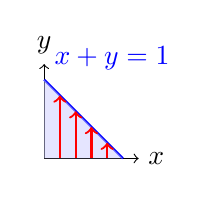
\begin{tikzpicture}
                    % 軸
                    \draw[->] (0,0) -- (1.2,0) node[right] {\(x\)};
                    \draw[->] (0,0) -- (0,1.2) node[above] {\(y\)};
                    
                    % 領域の境界 (y=x の線)
                    \draw[thick, blue] (1,0) -- (0,1) node[above right] {\(x+y=1\)};
                    
                    % 塗りつぶし領域
                    \fill[blue!20, opacity=0.5] (0,0) -- (1,0) -- (0,1) -- cycle;
                    
                    \foreach \x in {0.2, 0.4, 0.6, 0.8} {
                        \draw[->, red, thick] (\x,0) -- (\x,1-\x);
                    }
                \end{tikzpicture}
                \subcaption{解答の分割(y方向の分割)}
            \end{minipage}
            \begin{minipage}{0.45\columnwidth}
                \centering
                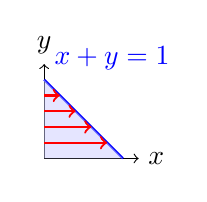
\begin{tikzpicture}
                    % 軸
                    \draw[->] (0,0) -- (1.2,0) node[right] {\(x\)};
                    \draw[->] (0,0) -- (0,1.2) node[above] {\(y\)};
                    
                    % 領域の境界 (y=x の線)
                    \draw[thick, blue] (1,0) -- (0,1) node[above right] {\(x+y=1\)};
                    
                    % 塗りつぶし領域
                    \fill[blue!20, opacity=0.5] (0,0) -- (1,0) -- (0,1) -- cycle;
                    
                    \foreach \y in {0.2, 0.4, 0.6, 0.8} {
                        \draw[->, red, thick] (0,\y) -- (1-\y,\y);
                    }
                \end{tikzpicture}
                \subcaption{x方向の分割}
            \end{minipage}
            \caption{(2)の領域と分割} \label{fig:多重積分:累次積分の分割の方向}
        \end{figure}

        累次積分を解く際には, 上図\ref{fig:多重積分:累次積分の分割の方向}のように, 図を書くとよい. なお, 次のように書いて解答してもよい.
        \begin{equation*}
            \iint_{x\geq0,y\geq0,x+y\leq 1}xdxdy=\int_0^1dx\int_{0}^{1-x}xdy=\int_{0}^{1}x(1-x)dx=\frac{1}{6}
        \end{equation*}
        こちらのほうが, 波かっこを書く分だけ手間が省けている.
    \clearpage
    \subsection{変数変換とJacobi行列式}
        ここでは変数変換について述べる. 一変数のとき, $x$についての積分を変数変換$x=g(t)$によって$t$の積分に帰着させる公式(置換積分)は, 
        \begin{equation}
            \int_{a}^{b}f(x)dx=\int_{t_a}^{t_b}(f\circ g)(t)\frac{dx}{dt}dt
        \end{equation}
        であった. このとき生じる係数$dx/dt$は変数変換による微小な長さ$dx$から$dt$への変換倍率であることは容易にわかる. 同様にして, 多重積分についても
        変数変換公式
        \begin{equation*}
            \iint_D f(x,y)dxdy=\iint_R f(x(u,v),y(u,v))Jdudv
        \end{equation*}
        および生じる係数$J$を求めたい, これがこの節の目標である.

        いきなり一般の変換に関して変換公式を求めるのは難しいから, ここでは一次変換
        \begin{equation}
            \left\{\begin{array}{c}
                x=Au+Bv\\
                y=Cu+Dv
            \end{array}\right. \label{eq:多重積分:一次変換}
        \end{equation}
        について考えてみる($A,B,C,D$は定数). 直感的に考えれば, 微小面積$dudv$はベクトル$(du,0),(0,dv)$のなすベクトルの面積であって, これらのベクトルを\eqref{eq:多重積分:一次変換}に
        よって変換前のベクトルは$(Adu,Bdu),(Cdv,Ddv)$であって, \eqref{eq:線形代数:二つのベクトルがなす面の面積}より
        \begin{equation*}
            dxdy=\left|\begin{vmatrix}Adu & Cdv \\ Bdu & Ddv\end{vmatrix}\right|=\left|\begin{vmatrix}A & C \\ B & D\end{vmatrix}\right|dudv
        \end{equation*}
        なることがわかる. ここで, すこし作為的だが, 次の変形をしてみることにしよう.
        \begin{equation*}
            \begin{vmatrix}A & C \\ B & D\end{vmatrix}=\begin{vmatrix}x_u & y_u \\ x_v & y_v\end{vmatrix}
        \end{equation*}
        このような行列式を\textbf{Jacobi行列式}\index{Jacobiぎょうれつしき@Jacobi行列式}, \textbf{Jacobian}\index{Jacobian}という. Jacobianは次の表記が主に用いられる.
        \begin{equation}
            J(u,v),\quad \frac{\partial(x,y)}{\partial(u,v)},\quad \frac{D(x,y)}{D(u,v)}
        \end{equation}

        今の議論は$dx,dy$などの微小量を用いた直感的な議論だったが, もちろんこれは簡単に精密化することができる. これはxy平面上の単位ベクトルとuv平面上の単位ベクトルの対応を考えればすぐわかるから, 
        演習問題にしよう.
        
        以上は一次変換の場合の変数変換だった. 問題は, 一般の変数変換$x=\phi(u,v),y=\psi(u,v)$である. 先に言ってしまうと, このときの変数変換の公式を厳密に求めるのはかなり難しい.
        かといって, いきなり公式だけ提示して終わるのはさすがに納得しずらいだろうから, これも直感的な説明をしようと思う.\footnote{残念ながら, この場合の直感的な説明は一次変換と違い, 簡単に厳密化はできない. そのためには面積確定など, 恐らく様々な概念の困難が立ちはだかるだろう.}
        
        先に, 一般の変数変換でも生じる係数はJacobianなのかを簡単に確かめてみる. 我々は以前全微分を学んでいた. これをうまくつかう. まず, 変数変換$x=\phi(u,v),y=\psi(u,v)$において, 全微分は$dx=\phi_udu+\phi_vdv, dy=\psi_udu+\psi_vdv$であった.
        これは一次変換の式\eqref{eq:多重積分:一次変換}と形式的に同じ形をしているから, $du,dv$が微小量であることより, 考えている微小面上で各係数は変化しないとすれば, 一次変換と同様の議論ができる. すなわち変数変換によって生じる係数は
        Jacobianに`なりそう'である.
        \clearpage
        つづいて, もう少し厳密にこの事実を確かめてみる. $x=\phi(u,v),y=\psi(u,v)$はそれぞれの変数を固定すれば, $x,y$を一つのパラメータ
        で表していることになり, これはxy平面上の曲線を意味する. それぞれの変数を固定して曲線を描き, それぞれさらに$v+\Delta v,u+\Delta u$だけずらしたものも描いた図は
        例えば以下のようになる.
        \begin{figure}[h]
            \centering
            \begin{tikzpicture}[scale=0.8]
                % 軸の描画
                \draw[->] (0,0) -- (6.5,0) node[right] {\(x\)};
                \draw[->] (0,0) -- (0,6) node[above] {\(y\)};
                
                \draw (1,4) .. controls (1.3,3) and (3,1.2) .. (4,1);
                \draw (2,5) .. controls (2.3,4) and (4,2.2) .. (5,2);

                \draw (4,5.3) .. controls (3.3,4) and (3,3.3) .. (1.5,2.3);
                \draw (5,4.3) .. controls (4.3,3) and (4,2.3) .. (2.5,1.3);

                \node[above] at (1,4) {$v$固定};
                \node[above] at (2,5) {$v+\Delta v$固定};

                \node[above] at (4.5,5.3) {$u+\Delta u$固定};
                \node[above] at (5,4.3) {$u$固定};

                \node[below] at (2.9,1.5) (A) {$A$};
                \node[below] at (1.8,2.5) (B) {$B$};                    
                \node[below] at (2.9,3.5) (C) {$C$};
                \node[below] at (4,2.5)   (D) {$D$};
            \end{tikzpicture}
            \caption{$u,v$をすこしだけ変化させたときの曲線の変化}
        \end{figure}

        このとき, $\Delta u,\Delta v$を十分小さく取れば, 曲線の交点を結んでできる図形の面積は$\Delta x\Delta y$と等しい.
        また, この図形の面積は, この図形がベクトル$\vec{AB},\vec{AD}$のなす面であるから, \eqref{eq:線形代数:二つのベクトルがなす面の面積}より
        \begin{equation*}
            \Delta x\Delta y\sim\left|\begin{vmatrix}\phi(u+\Delta u,v)-\phi(u,v) & \phi(u,v+\Delta v)-\phi(u,v) \\ \psi(u+\Delta u,v)-\psi(u,v) & \psi(u,v+\Delta v)-\psi(u,v)\end{vmatrix}\right|=\left|\begin{vmatrix}\phi_u\Delta u & \phi_v\Delta v \\ \psi_u\Delta u & \psi_v\Delta v\end{vmatrix}\right|=|J(u,v)|\Delta u\Delta v
        \end{equation*}
        ここで途中の計算では平均値の定理を用いた. \footnote{この時例えば, $\phi_u=\phi_u(u+\theta\Delta u,v)$であるが, $\Delta u\to 0$の過程で$\theta\Delta u\to 0$であるから気にしなくてよい.}
        よって, $\Delta u,\Delta v \to 0$のとき, 等号が成り立つから, 面積比としては$|J|$が生じるのである.

        以上がすこしだけ厳密な証明であった. 数学的に完全に厳密に示すには, 適当な解析の本を参照してほしいと思う. すくなくとも, 名著解析概論と杉浦解析には書いていた.
        変数変換は, 公式の証明も大事であるが, どちらかといえば公式を使いこなすことに重点が置かれる. このノートでも次の頁以降で基本的な座標変換に対するJacobianとその計算法について述べる.

        以下, 改めて変数変換の公式を書いておこう.
        \begin{equation}
            \iint_D f(x,y)dxdy = \iint_R f(x(u,v),y(u,v))|J(u,v)|dudv \label{eq:多重積分:変数変換の公式}
        \end{equation}
        なお, 以上の議論は三重積分にも, もっと一般に$N$重積分においても同様であって, 変換公式も同様になる. その場合, Jacobianは$N$次関数行列式になる.
        \clearpage
        さて, 次に我々が扱いたいのは直交座標から特定の座標への変換である. もっともよく扱われるのは極座標系であろうから, まずは極座標変換について考えたい. まずは二次元平面上での変換を考える.
        二次元平面上の直交座標から極座標への変換は, 以下の式で与えられる.
        \begin{equation}
            x=r\cos\theta, y=r\sin\theta \quad (r\geq 0,0\leq \theta<2\pi) \label{eq:多重積分:平面極座標変換}
        \end{equation}
        これは以下の図から容易にわかるだろう.
        \begin{figure}[h]
            \centering
            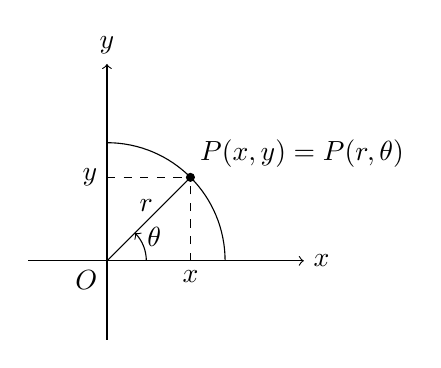
\begin{tikzpicture}
                \draw[->] (-1,0) -- (2.5,0);
                \draw[->] (0,-1) -- (0,2.5);

                \node[below left] at (0,0) {$O$};
                \node[right] at (2.5,0) {$x$};
                \node[above] at (0,2.5) {$y$};

                \draw (1.5,0) arc[radius=1.5, start angle=0, end angle=90];
                \draw (0,0) -- (1.06,1.06) node[above right] {$P(x,y)=P(r,\theta)$};
                \draw[fill=black] (1.06,1.06) circle[radius=0.05];
                \draw[->] (0.5,0) arc[radius=0.5, start angle=0, end angle=45];
                \draw[dashed] (0,1.06) -- (1.06,1.06);
                \draw[dashed] (1.06,0) -- (1.06,1.06);
                \node[below] at (1.06,0) {$x$};
                \node[left]  at (0,1.06) {$y$};
                \node[above] at (0.5,0.5) {$r$};
                \node at (0.6,0.3) {$\theta$};
            \end{tikzpicture}
            \caption{直交座標系と極座標系の関係}
        \end{figure}

        この動径$r$と角度$\theta$の組$(r,\theta)$で平面上の点を表現する座標を\textbf{極座標}\index{きょくざひょう@極座標}といい, 
        \eqref{eq:多重積分:平面極座標変換}の変換を\textbf{極座標変換}\index{きょくざひょうへんかん@極座標変換}という. 直交座標で考えると難しい問題も,
        極座標に変換しておくと簡単に解ける, といったことがある. 

        さっそく, 極座標変換におけるJacobi行列式を求めてみよう.
        \begin{equation*}
            J(r,\theta)=\begin{vmatrix}\partial_r(r\cos\theta) & \partial_r (r\sin\theta) \\ \partial_\theta (r\cos\theta) & \partial_\theta (r\sin\theta) \end{vmatrix}
            =\begin{vmatrix}\cos\theta & \sin\theta \\ -r\sin\theta & r\cos\theta\end{vmatrix}=r
        \end{equation*}
        したがって, 重積分の極座標変換は以下のようになる.
        \begin{equation}
            \iint_D f(x,y)dxdy = \iint_R f(r\cos\theta,r\sin\theta)rd\theta dr\label{eq:多重積分:重積分の極座標変換}
        \end{equation}
        実は, この二次元極座標変換における微小面積の変換$dxdy=rd\theta d\theta$は, Jacobianを用いない直感的な導出ができる.
        下図において, 赤い枠で囲まれた図形の面積が微小面積$dxdy$である. 一方, この面積は, 横の長さ$rd\theta$, 縦の長さ$dr$の長方形と近似することができるから, 
        $dxdy=rd\theta dr$となる.
        \begin{figure}[h]
            \centering
            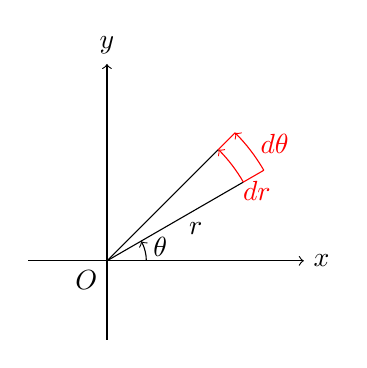
\begin{tikzpicture}
                \draw[->] (-1,0) -- (2.5,0);
                \draw[->] (0,-1) -- (0,2.5);

                \node[below left] at (0,0) {$O$};
                \node[right] at (2.5,0) {$x$};
                \node[above] at (0,2.5) {$y$};

                \draw (0,0) -- (30:2);
                \draw[color=red,->] (30:2) arc[radius=2,start angle=30,end angle=45];
                \draw (0,0) -- (45:2);

                \draw[color=red] (30:2) -- (30:2.3);
                \draw[color=red,->] (30:2.3) arc[radius=2.3,start angle=30,end angle=45];
                \draw[color=red] (45:2) -- (45:2.3);

                \node at (20:1.2) {$r$};
                \node[color=red] at (25:2.1) {$dr$};
                \node[color=red] at (35:2.6) {$d\theta$};
                \draw[->] (0.5,0) arc[radius=0.5,start angle=0,end angle=30];
                \node at(15:0.7) {$\theta$};
                
            \end{tikzpicture}
            \caption{微小面積変換の直感的な導出}
        \end{figure}
        \clearpage
        試しに, 極座標変換を用いて重積分を計算してみよう.
        \begin{equation*}
            \iint_{x^2+y^2\leq 1}xdxdy=\iint_{0\leq r\leq 1,0\leq\theta<2\pi}r\cos\theta rd\theta dr = \int_{0}^{2\pi}\cos\theta d\theta\int_{0}^{1}r^2dr=0
        \end{equation*}
        実際グラフを考えれば, これは$x>0$と$x<0$の領域が対称的だから, 確かに0になることがわかる.\\

        最後に, 三次元の座標変換, 特に\textbf{球面座標}\index{きゅうめんざひょう@球面座標}への変換を考えてみよう. 球面座標変換は, 以下の式で与えられる.
        \begin{equation}
            x=r\sin\theta\cos\phi, y=r\sin\theta\sin\phi, z=r\cos\theta \quad (r\geq 0,0\leq\phi<2\pi,0\leq\theta\leq \pi) \label{eq:多重積分:球面座標変換}
        \end{equation}
        この関係も, 図\footnote{実は当初この図ではなく, tikz-3dplotの\href{https://ctan.math.washington.edu/tex-archive/graphics/pgf/contrib/tikz-3dplot/tikz-3dplot_documentation.pdf}{リファレンス}のサンプルコードから書く予定だったのだが,
        どうにもうまくいかず, いろいろ試行錯誤した末, 以前(ベクトル解析の問題作成用に)書いていたものを流用する形となった. 過去の自分に感謝した.}を見れば容易にわかる.
        \begin{figure}[h]
            \centering
            \begin{tikzpicture}
                \coordinate (A) at (2,0,2);
                \coordinate (P) at (2,2,2);
                \coordinate (O) at (0,0,0);
                \coordinate (X) at (0,0,2);
                \coordinate (Y) at (0,2,0);
                \draw[->] (O) -- (P);
                \draw[->,thick] (O) -- (2,0,0); 
                \draw[->,thick] (O) -- (X); 
                \draw[->,thick] (O) -- (Y); 
                \draw[dashed] (P) -- (A);
                \draw[dashed] (O) -- (A);
                \node[left] at (P) {$r$};
                \draw pic["$\theta$", draw, font=\footnotesize, angle eccentricity=1.3, angle radius=0.5cm] {angle=P--O--Y};
                \draw pic["$\phi$", draw, font=\footnotesize, angle eccentricity=1.5, angle radius=0.3cm] {angle=X--O--A};
                \node[left] at (0,0,2) {$x$};
                \node[left] at (0,2,0) {$z$};
                \node[above] at (2,0,0) {$y$};
            \end{tikzpicture}
            \caption{直交座標系と球面座標の関系}
        \end{figure}

        これより, Jacobi行列式は
        \begin{equation*}
            \frac{\partial(x,y,z)}{\partial(r,\phi,\theta)}=
            \begin{vmatrix}
                x_r & y_r & z_r \\
                x_\phi & y_\phi & z_\phi\\
                x_\theta & y_\theta & z_\theta
            \end{vmatrix}
            =
            \begin{vmatrix}
                \sin\theta\cos\phi & \sin\theta\sin\phi & \cos\theta \\
                -r\sin\theta\sin\phi & r\sin\theta\cos\phi & 0\\
                r\cos\theta\cos\phi & r\cos\theta\sin\phi & -r\sin\theta
            \end{vmatrix}
            =r^2\sin\theta \label{eq:多重積分:球面座標のヤコビアン}
        \end{equation*}
        となる. さっそくこれを用いて, 球の体積を求めてみよう.
        \begin{equation*}
            \iiint_{x^2+y^2+z^2\leq R^2}dxdydz=\int_{0}^{2\pi}d\phi\int_{0}^{\pi}d\theta\int_{0}^{R}r^2\sin\theta dr=2\pi\cdot 2\cdot \frac{R^3}{3}=\frac{4\pi R^3}{3}
        \end{equation*}
        このように, 中学時代暗記に苦労した球の体積の公式も簡単に求まってしまう. 球面座標変換の威力である. なお, 球の体積自体は, 通常の一次元の積分および重積分からも求めることができることに注意しておく.
    \clearpage
    \subsection{Gauss積分}
        最後に, 有名な積分公式を一つ紹介しておこう.
        \begin{equation}
            \int_{-\infty}^{\infty}e^{-x^2}dx = \sqrt{\pi}\label{eq:多重積分:ガウス積分}
        \end{equation}
        これがいわゆる\textbf{Gauss積分}\index{Gaussせきぶん@Gauss積分}であって, 理工学や統計で重要な地位を占める. 
        統計を少しでもかじったことがある人は, 正規分布の確率密度関数がこの被積分関数を変数変換したものであり, 全体の確率が1
        になるよう規格化されたものであると気づくだろう. もちろん, 数学においても到る所に顔を出す重要な積分で, 例えば複素解析で解くであろう
        有名な積分の多くは, このGauss積分の結果を用いる. そうでなくても, 不定積分ができない関数でも定積分が計算されるという一つの実例になっていることは
        数学的に大変興味深いことである. うすうす気づかれている読者もいるだろうが, この積分の定積分が計算できる, とはいっても一変数の積分だけで計算するのはなかなかに骨が折れる.
        もちろん, この積分の結果が$\sqrt{\pi}$であることを知っているならば, 適当な不等式評価によってこの公式を証明することができるだろう.
        しかしそれはあくまで答えを知っていたからできる芸当であって, 実際の導出としてはかなり不自然である. そこでここでは, 我々が学んだ重積分の知識を用いてこの積分を計算してみたいと思う.

        まず, この広義積分が収束することを確認しておこう. 評価を簡単にするために, $[0,\infty)$で考える. まず, $x\to\infty$で$e^{-x^2}$よりも$e^{-x}$のほうが増加のスピードは早いことから,
        適当な$x_0>0$を取れば$x\geq x_0$で$e^{-x}\geq e^{-x^2}$と出来る. したがって
        \begin{equation*}
            \int_{x_0}^{\infty}e^{-x^2}dx\leq \int_{x_0}^{\infty}e^{-x}dx = e^{x_0} < \infty
        \end{equation*}
        であるから, 元の積分も収束することがわかる. \footnote{被積分関数は常に正だから, この原始関数は常に単調増加であって, 上記で述べたことより有界であるから, これは有限値に収束するのである.}
        よって, 次の変形を行う.
        \begin{equation*}
            \left(\int_{0}^{\infty}e^{-x^2}dx\right)^2 = \left(\int_{0}^{\infty}e^{-x^2}dx\right)\cdot \left(\int_{0}^{\infty}e^{-x^2}dx\right)=\left(\int_{0}^{\infty}e^{-x^2}dx\right)\cdot \left(\int_{0}^{\infty}e^{-y^2}dy\right)=\int_0^\infty dx\int_0^\infty e^{-x^2-y^2}dy
        \end{equation*}
        これは累次積分の形であるから, これを重積分に戻すことを考える. 積分範囲は, xy平面の第一象限全体であるから, これを次の積分範囲の極限とみなす.
        \begin{equation*}
            D_R = \{(x,y)\mid x^2+y^2\leq R^2,x\geq 0,y\geq 0\}
        \end{equation*}
        すなわち, 以下の重積分へと書き換えられる.
        \begin{equation*}
            \lim_{R\to\infty}\iint_{D_R} e^{-(x^2+y^2)}dxdy
        \end{equation*}
        さて, これによって, 一次元積分の問題が, 重積分の問題へと帰着されたわけであるが, これはどのように解けばよいだろうか. 
        積分領域と被積分関数をすこし眺めれば, これが極座標変換の問題であると気づくだろう.(実際そのための領域を取っている.)
        そこで, 極座標変換によって重積分を計算すれば, $0\leq\theta\leq\frac{\pi}{2}$に注意して
        \begin{equation*}
            \lim_{R\to\infty}\iint_{D_R} e^{-(x^2+y^2)}dxdy = \lim_{R\to\infty}\int_{0}^{\frac{\pi}{2}}d\theta\int_{0}^{R}re^{-r^2}dr=\lim_{R\to\infty}\frac{\pi}{4}\left[1-e^{-R^2}\right]=\frac{\pi}{4}
        \end{equation*}
        \clearpage
        したがって, 次の式が得られたことになる.
        \begin{equation*}
            \left(\int_{0}^{\infty}e^{-x^2}dx\right)^2 = \frac{\pi}{4}
        \end{equation*}
        後はこれを変形して, 積分区間を元に戻せば\eqref{eq:多重積分:ガウス積分}が得られる.\\

        この計算は厳密には多重積分の広義積分に属するもので, 広義積分を計算する場合はもう少し慎重に考える必要がある. しかし, ここではその厳密な方法を述べない. 大抵の場合は, 厳密なことに拘らなくても計算することが可能であるし, 
        そのほうが計算に集中することができるからである. また必要な時に厳密な定理を学べばよい. なお, Gauss積分は極座標変換を用いなくとも, 単なる重積分だけで求めることもできるので, 時間と余力がある場合は考えてみるとよい. かなり技巧的である.\\\\

        以上で多重積分について大まかに述べた. これでこの第I部は終了であるが, QuuNoteIと比べてかなりページ数が多いことに気が付くだろう.
        本来これらそれぞれの節の内容がそれぞれ独立して部として書くことができるほど内容が多いのだが, ここでは後のことを考えて小節としたのである.
        そのため, 普通の微分積分の教科書に書いてあるだろう定理や公式も省略していることが多い. もし知識の不足で不安ならば適当な微分積分の教科書を読んでみてほしい.
        \clearpage
        \basicquestion 以下の問いに答えよ。

        \subsubsection*{問1} 次の重積分を計算せよ.\\
            $(1)\displaystyle \int_{0}^{1}dy\int_{0}^{1}(x+y)dx$\hspace{5mm}
            $(2)\displaystyle \int_{0}^{1}dx\int_{0}^{\sqrt{1-x^2}}\sqrt{1-x^2}dy$

        \subsubsection*{問2} 次の三重積分を計算せよ.\\
            $(1)\displaystyle \int_{0}^{1}dz\int_{0}^{2}dy\int_{1}^{3}dx$\hspace{5mm}
            $(2)\displaystyle \int_{0}^{1}dx\int_{z}^{1}dy\int_{z+y}^{1}ydx$\hspace{5mm}
            $(3)\displaystyle \int_{0}^{\pi}dz\int_{0}^{\sin z}dx\int_{x^2}^{1}\cos zdy$

        \subsubsection*{問3}次の領域における重積分を計算せよ.\\
            $(1)\displaystyle \iint_D (x+y)^2dxdy\quad [D:x+y\leq 1,x\geq0,y\geq0]$\hspace{1mm}
            $(2)\displaystyle \iint_D e^{y^2}dxdy\quad [D:0\leq x\leq 1,x\leq y\leq 1]$

            \noindent
            $(3)\displaystyle \iint_D(x+y)\sin\pi(x-y)dxdy\quad [D:0\leq x+y\leq 1,0\leq x-y\leq 1]$

            \noindent
            $(4)\displaystyle\iint_D \frac{dxdy}{x^2+y^2} \quad [D:1\leq x^2+y^2\leq 4]$
        
        \subsubsection*{問4} 次の領域における三重積分を計算せよ. ただし$V:x+y+z\leq 1,x\geq 0, y\geq 0,z\geq 0$とする.\\
            $(1)\displaystyle \iiint_V \frac{dxdydz}{(x+y+z+1)^3}$\hspace{5mm}
            $(2)\displaystyle \iiint_V (x^2+y^2+z^2)dxdydz$\hspace{5mm}
            $(3)\displaystyle \iiint_{x^2+y^2+z^2\leq 1}x^2dxdydz$

        \subsubsection*{問5}重積分$\displaystyle\iint_{\frac{x^2}{a^2}+\frac{y^2}{b^2}\leq 1}xydxdy $を求めよ. (適当な変数変換を考えよ.)
        \vspace{-0.5cm}

        \subsubsection*{問6}一次変換\eqref{eq:多重積分:一次変換}におけるJacobianの導出(同頁参照)において, xy平面上の単位正方形の面積はuv平面の単位正方形の$|J|$倍であることを証明せよ.
        \vspace{-0.5cm} 

        \subsubsection*{問7}一変数の積分と違い, 変数変換公式\eqref{eq:多重積分:変数変換の公式}において生じる係数$|J|$にはなぜ絶対値がついているのだろうか.
        \vspace{-1cm} 

        \subsubsection*{問8}領域$V$上に密度$\rho(x,y,z)$で広がる物体が回転運動する際の慣性モーメントは, 回転軸の長さを$l(x,y,z)$として
            \begin{equation}
                I=\iiint_{V}\rho(x,y,z)l(x,y,z)^2dxdydz
            \end{equation}
            と与えられる. 半径$R$, 質量$M$の球を重心を通るz軸の回りに回転させることを考えたとき, この時の慣性モーメントを求めよ.\footnote{慣性モーメントの物理的な意味は力学の本を参照.}
        \clearpage
    \section{第I部演習問題}
        \subsubsection*{問1} $\varepsilon-N$論法の否定命題を示せ.

        \subsubsection*{問2} 区間$I=[0,1]$における狭義単調増加関数$f$は, その$f(I)$を値域とするとき全単射であることを示せ. 

        \subsubsection*{問3} 単調増加な集合列$A_n$, すなわち$A_1\subset A_2\subset\cdots$が成り立つとき, 
            \begin{equation}
                \lim_{n\to\infty} A_n = \bigcup_{n=1}^\infty A_n
            \end{equation}
            であり, 単調減少な集合列$B_n$, つまり$B_1\supset B_2 \supset \cdots$が成り立つとき
            \begin{equation}
                \lim_{n\to\infty} B_n = \bigcap_{n=1}^\infty B_n
            \end{equation}
            であることを示せ.
        
        \subsubsection*{問3} 実数$\mathbb{R}$に$\infty,-\infty$も含めて拡張した$\overline{\mathbb{R}}$を考える. このとき, $\overline{\mathbb{R}}$上の任意の広義の単調列は収束することを示せ.

        \subsubsection*{問4} 回転を表す行列\eqref{eq:線形代数:回転行列}を$R(\theta)$と書くとき, $R^n(\theta)=R(n\theta)\quad (n\in\mathbb{N})$を示せ.

        \subsubsection*{問5} 行列$\displaystyle A=\begin{pmatrix}1&2&3\\-2&-3&-4\\2&2&4\end{pmatrix}$ は正則であるか? もし正則ならば逆行列を求めよ.

        \subsubsection*{問6} $u=(x\cos\alpha-y\sin\alpha)/(x^2+y^2),\quad v=(x\sin\alpha+y\cos\alpha)/(x^2+y^2)$とするとき, $u_x+v_y$を求めよ.

        \subsubsection*{問7} 座標の添え字を上に書き, $x=x^0,y=x^1,z=x^2$とする. (べき乗の意味ではない. 詳しくは第IV部参照.) 座標変換$(x^1,x^2,x^3)\to (x'^1,x'^2,x'^3)$を行うことで, 全微分は次のように変換されることを確かめよ.
            \begin{equation*}
                dx'^i = \sum_{j=1}^{3}\frac{\partial x'^i}{\partial x^j}dx^j
            \end{equation*}
        
        \subsubsection*{問8} $f(x,y)=x^3+y^3+(x+y)^2$の極値を全て求めよ.

        \subsubsection*{問9} 以下の問いに答えよ.
            \begin{enumerate}\renewcommand{\labelenumi}{(\roman{enumi})}
                \item $\displaystyle \int_{0}^{\infty}e^{-\alpha x}dx \quad (\alpha>0)$を計算せよ.
                \item $\frac{1}{\alpha^n}$を定積分で表せ. ただし$n$は自然数.
            \end{enumerate}
        
        \subsubsection*{問10} $D$を三点$(0,0),(\pi,0),(0,\pi)$を頂点とする三角形とするとき, $\displaystyle \iint_D \frac{y\sin x}{x}dxdy$を求めよ.
        
        \subsubsection*{問11} $D:0\leq y\leq \sqrt{3}x,x^2+y^2\leq 4$とする. この時$\displaystyle \iint_D xdxdy$を求めよ.

        \subsubsection*{問12} x軸上の微小線素$dx$に点が存在する確率を$\frac{1}{\sqrt{2\pi}\sigma}e^{-x^2/2\sigma^2}dx$とし, 同様の独立した分布が$y$軸上にも存在しているとする. 次の問いに答えよ.
            \begin{enumerate}\renewcommand{\labelenumi}{(\roman{enumi})}
                \item xy平面上の微小面積$dxdy$に点が存在する確率$dP$を求めよ.
                \item このときの点の原点からの距離の期待値$E$は, $E=\displaystyle\int_{\mathbb{R}^2}\sqrt{x^2+y^2}dP$で与えられる. $E$を計算せよ.
            \end{enumerate}
            各軸上の分布は正規分布$N(0,\sigma^2)$である. なお, $\int_{\mathbb{R}^2}$はxy平面全体で積分の意.